% % % % % % % % % % % % % % % % % % % % % % % % % % % % % % % % % % % % % % % %
% LaTeX4EI Example for Cheat Sheets
%
% @encode: 	UTF-8, tabwidth = 4, newline = LF
% @author:	LaTeX4EI
% % % % % % % % % % % % % % % % % % % % % % % % % % % % % % % % % % % % % % % %

% This summary was taken from Sebastian Schweizer, and adapted to C++ and more. 

% ======================================================================
% Document Settings
% ======================================================================

% possible options: color/nocolor, english/german, threecolumn
% default: color, english
\documentclass[german]{latex4ei/latex4ei_sheet}
\usepackage{multirow}
\usepackage{graphicx}
\usepackage{amsmath}
\usepackage{amsfonts}
\usepackage{amssymb}
\usepackage{tabularx}
\usepackage{pbox}
\usepackage{nicefrac}
\usepackage{listings}
\usepackage{wrapfig}

%\renewcommand{\vec}[1]{\underline{#1}}
\newcommand\tab[1][.3cm]{\hspace*{#1}}

% set document information
\title{Zusammenfassung Informatik II}

\author{Nic Cantieni}					% optional, delete if unchanged
\myemail{ncantieni@ethz.ch}			% optional, delete if unchanged

% DOCUMENT_BEGIN ===============================================================
\begin{document}

\maketitle

% SECTION ====================================================================================
\section{Algorithmen und Datenstukturen}
% ============================================================================================

\begin{sectionbox}
\subsection{Terminologie}\par\smallskip
\textbf{Algorithmus}: Wohldefinierte Berechnungsvorschrift, welche aus Eingabedaten (input/Probleminstanz) Ausgabedaten (output) berechnet.\par\smallskip
\textbf{Datenstrukturen}: Eine Datenstruktur organisiert Daten so in einem Computer, dass man sie (in den
darauf operierenden Algorithmen) effizient nutzen kann.\par\smallskip
\textbf{Effizienz}: Die Effizienz eines Algorithmus ist seine Sparsamkeit bezüglich der Ressourcen, Zeit und Speicherplatz, die er zur Lösung eines festgelegten Problems beansprucht.
\end{sectionbox}

\begin{sectionbox}
\subsection{Effizienz von Algorithmen}\smallskip
%\begin{center}
%    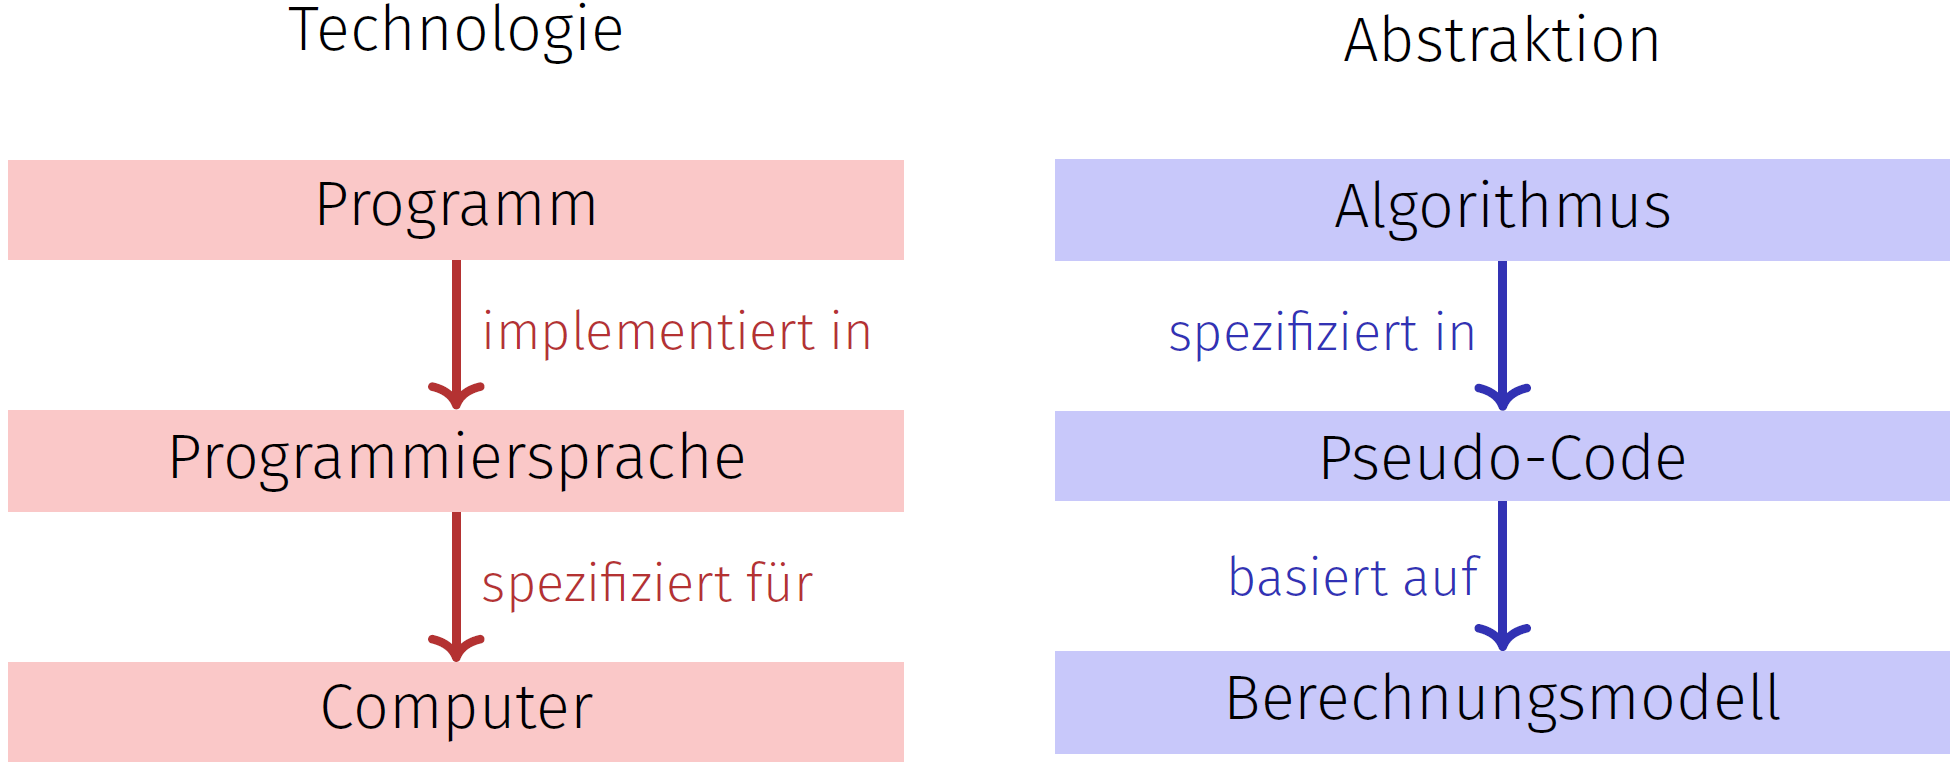
\includegraphics[width = 0.9\columnwidth]{../img/AbstraktionProgramm.png}
%\end{center}\par\smallskip

\textbf{Asymptotische Laufzeiten}\par
\begin{itemize}
    \item \textbf{Obere Schranke}: $\mathcal{O}(g)=\{f:\mathbb{N} \rightarrow \mathbb{R}\ |\ \exists c>0, \exists n_{0} \in \mathbb{N}:$\par $\forall n \geq n_{0}: 0 \leq f(n) \leq c \cdot g(n)\}$
    \item \textbf{Untere Schranke}: $\Omega(g)=\{f: \mathbb{N} \rightarrow \mathbb{R}\ |\ \exists c>0, \exists n_{0} \in \mathbb{N}:$ \par $\forall n \geq n_{0}: 0 \leq c \cdot g(n) \leq f(n)\}$
    \item \textbf{Scharfe Schranke}: $\Theta(g):=\Omega(g) \cap \mathcal{O}(g)$\par
    $\Theta(f) = \{  g: \N \rightarrow \R\ |\ \exists c>0,\ \exists n_0 \in \N:$\par $\forall n \geq n_0: 0 \leq \frac1c \cdot f(n)\leq g(n) \leq c \cdot f(n)\}$
\end{itemize}\par\smallskip

\begin{greenbox}
\textbf{Theorem}\par
Seien $f, g: \mathbb{N} \rightarrow \mathbb{R}^{+}$ zwei Funktionen. Dann gilt.
\begin{enumerate}
    \item $\lim _{n \rightarrow \infty} \frac{f(n)}{g(n)}=0 \Rightarrow f \in \mathcal{O}(g), \mathcal{O}(f) \subsetneq \mathcal{O}(g)$
    \item $\lim _{n \rightarrow \infty} \frac{f(n)}{g(n)}=C>0\ (C \text { konstant}) \Rightarrow f \in \Theta(g)$
    \item $\frac{f(n)}{g(n)} \underset{n \rightarrow \infty}{\longrightarrow} \infty \Rightarrow g \in \mathcal{O}(f), \mathcal{O}(g) \subsetneq \mathcal{O}(f)$
\end{enumerate}
\end{greenbox}\smallskip
\textit{Beispiel aufsteigende Laufzeiten:}\par
$ 2^{16},\ \log(n^4),\ \log^8(n),\ \sqrt{n},\ n\log n,\ \binom{n}{3},\ n^5+n,\ \frac{2^n}{n^2},\ n!,\ n^n$\par\smallskip

\textbf{Analyse mit Rekurenz und Teleskopie}\par\vspace{-4px}
\begin{lstlisting}[language=Java]
void g(int n) {
    if (n>1) {
        g(n/2);
        g(n/2);
    }
    else {
        f();
    }
}
\end{lstlisting}\vspace{-4px}
\textit{Rekurrenz} ($n=2^{i}$)\par
$T(n)=\left\{\begin{array}{ll}2 T(n / 2) & n>1 \\ 1 & n=1\end{array}\right.$\par\smallskip
\textit{Teleskopieren}\par
$T(n)=2 \cdot T(n / 2) = 2 \cdot (2 \cdot T(n / 4)) $ \par
$= 2^{i} \cdot T(n/2^{i}) = n \cdot T(n/n) \in \Theta(n)$\par\smallskip

\end{sectionbox}

% SECTION ====================================================================================
\vspace{-4pt}
\begin{sectionbox}
\section{Suchen}
% ============================================================================================
\subsection{Divide and Conquer}\smallskip
\begin{tabular*}{\columnwidth}{@{\extracolsep\fill}ll@{}}
Gegeben: & Sortiertes Array $A$ mit $n$ Elementen und einen Schlüssel b \\
Gesucht: & Index k mit $A[k]=b$ \\
Lösung: & Zeiger und Halbierung des Arrays\\
\end{tabular*}

\begin{center}
    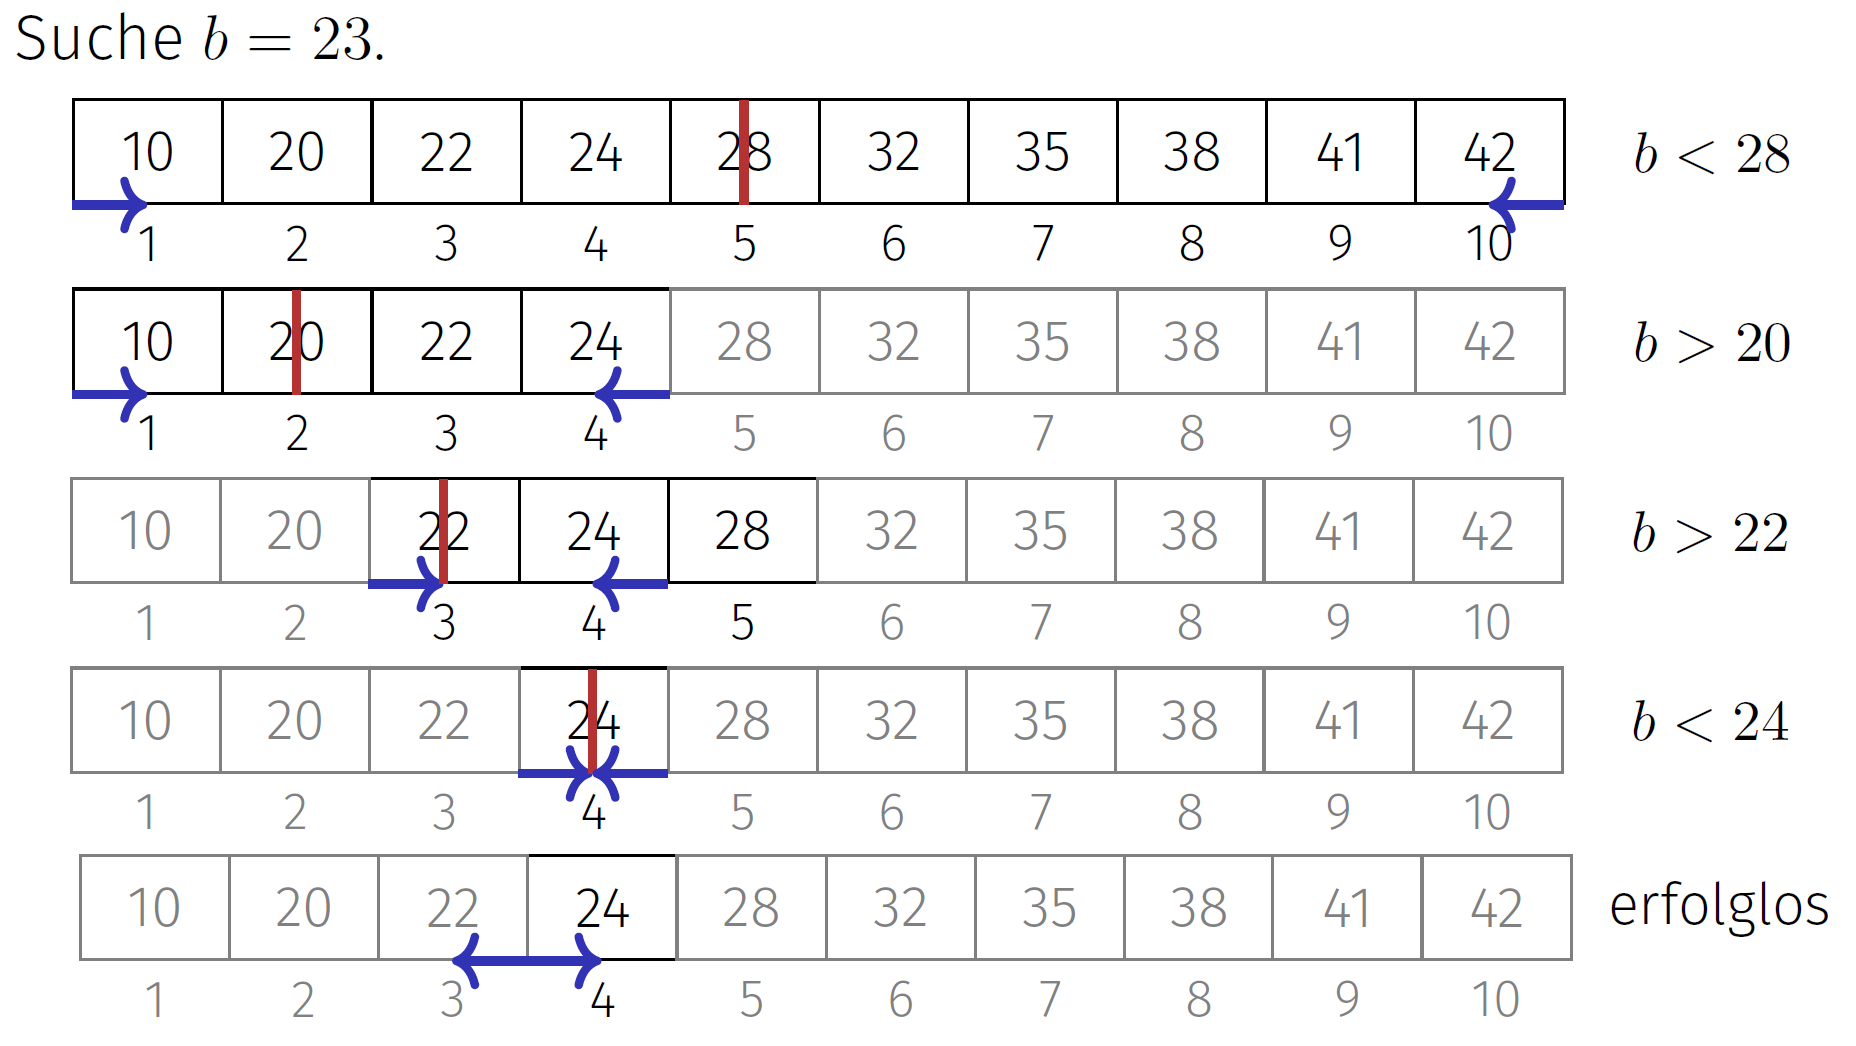
\includegraphics[width = 0.6\columnwidth]{../img/DaQ.png}
\end{center}\par\smallskip
\end{sectionbox}
\vspace{-4pt}
\begin{sectionbox}
\subsection{Binärer Suchalgorithmus: BSearch(A,l,r,b)}\smallskip
\begin{center}
    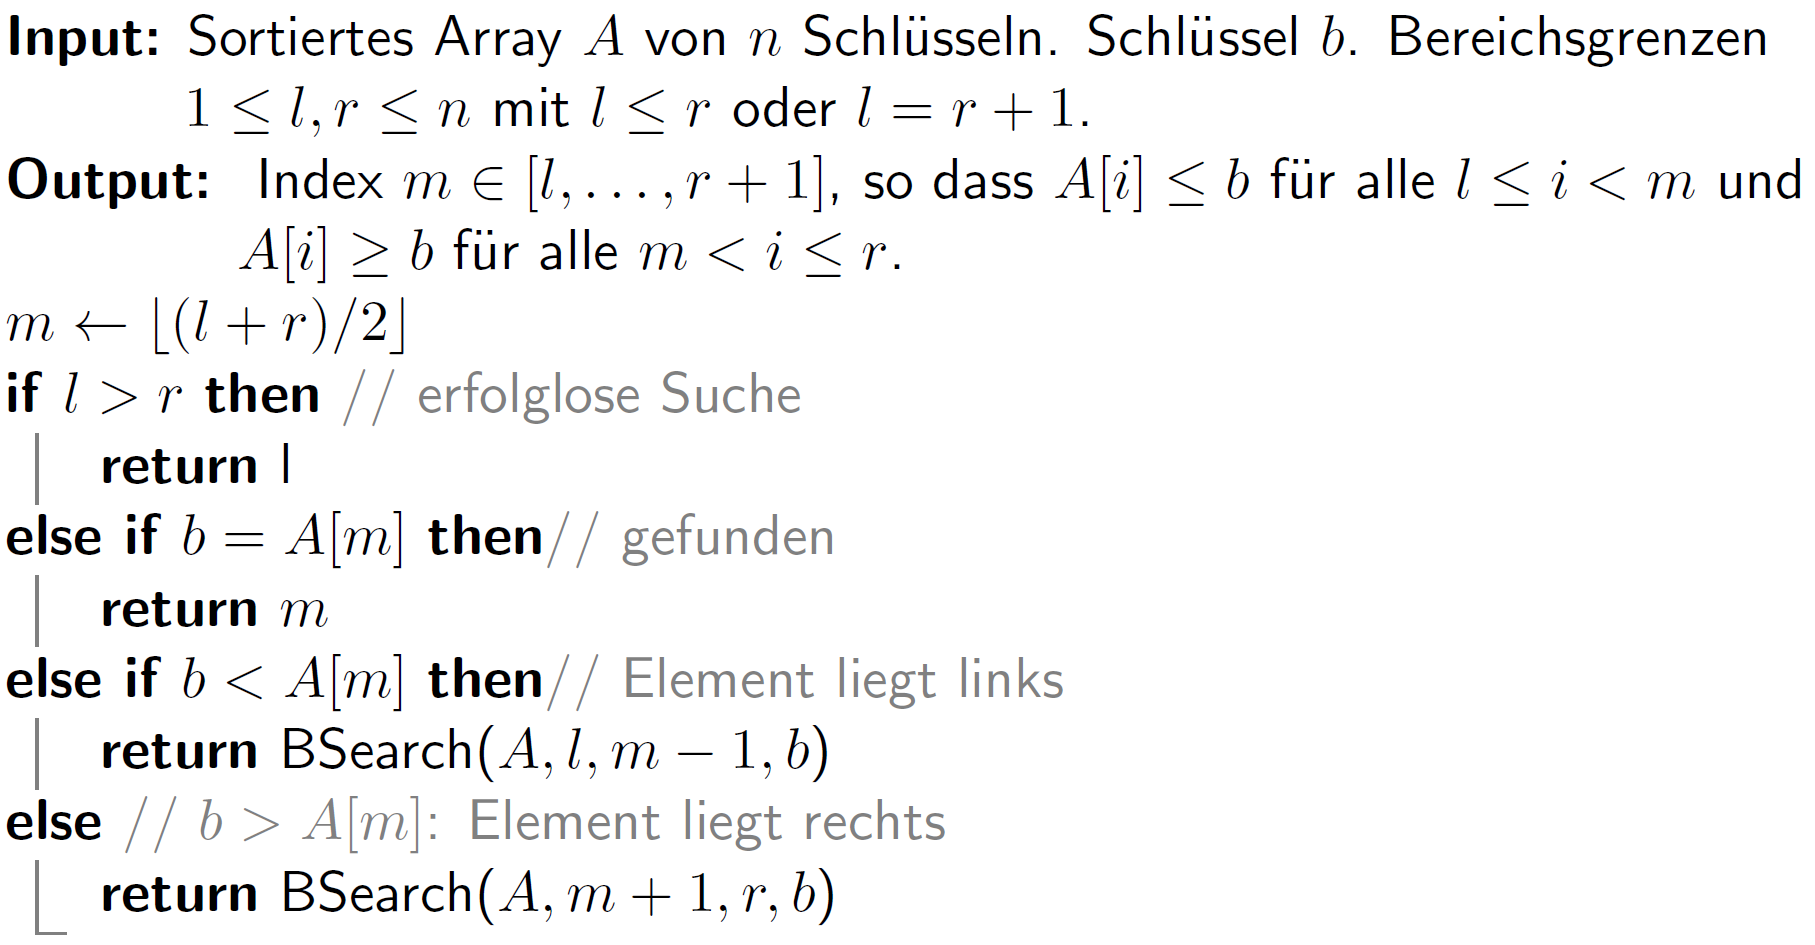
\includegraphics[width = \columnwidth]{../img/BSearch.png}
\end{center}\par\smallskip
\end{sectionbox}

% SECTION ====================================================================================
\section{Sortieren}
% ============================================================================================

\begin{sectionbox}
\subsection{Laufzeiten von Sortier-Algorithmen}\smallskip
\begin{center}
    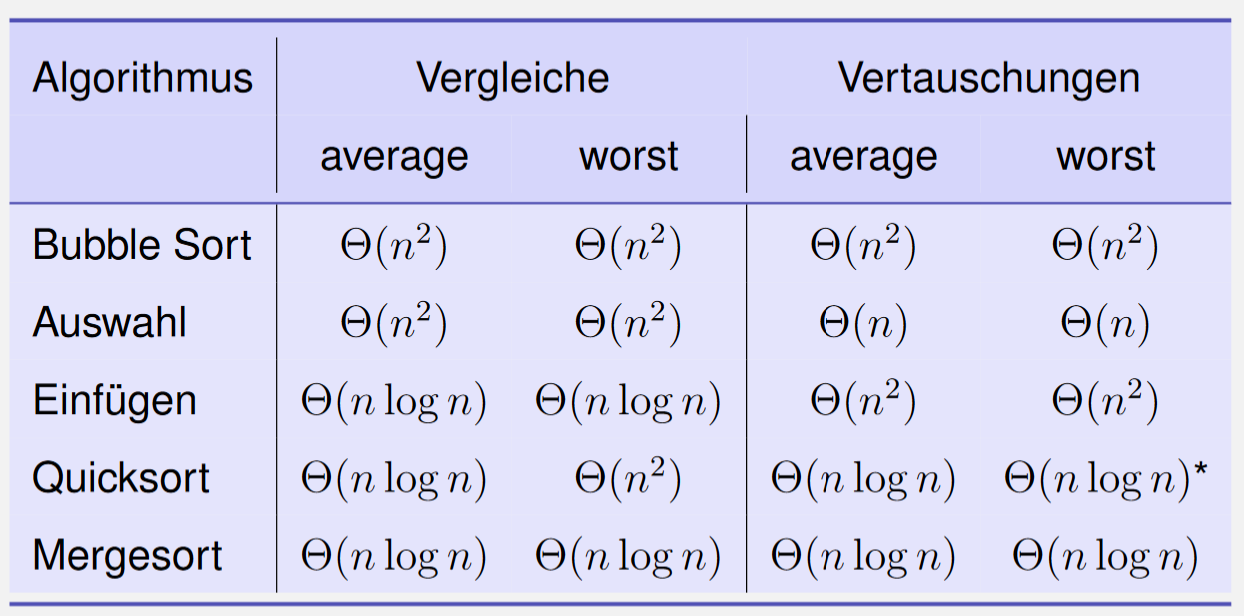
\includegraphics[width = \columnwidth]{../img/LaufzeitenSort.png}
\end{center}
\end{sectionbox}

\begin{sectionbox}
\subsection{Bubble-Sort}
\begin{lstlisting}[language=Python]
def bubbleSort(arr): 
    n = len(arr) 
    for i in range(n):
        for j in range(n-i-1): 
            if arr[j] > arr[j+1] : 
                arr[j], arr[j+1] = arr[j+1], arr[j] 
\end{lstlisting}\vspace{-6px}
\end{sectionbox}

\begin{sectionbox}
\subsection{Sortieren durch Auswahl}\smallskip
\begin{tabular*}{\columnwidth}{@{\extracolsep\fill}ll@{}}
\multirow{9}{*}{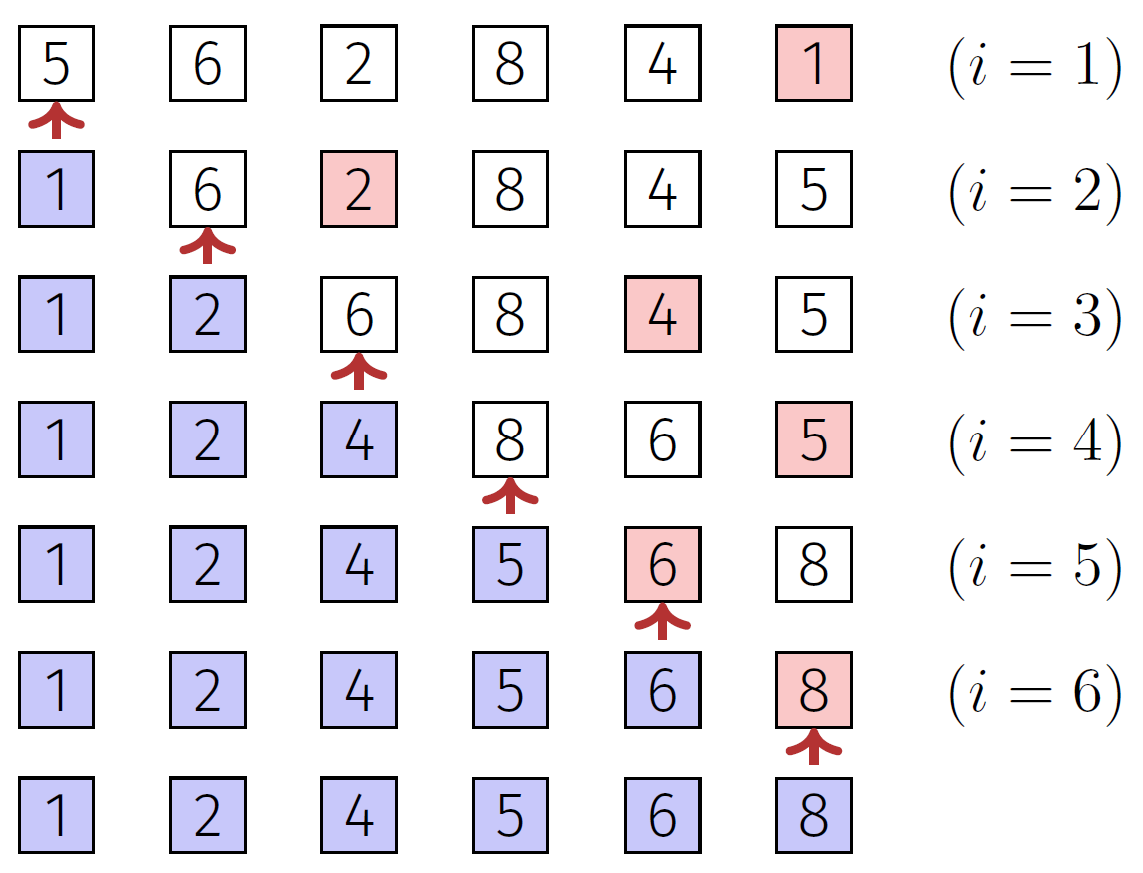
\includegraphics[width = 0.5\columnwidth]{../img/selectSort.png}}
& Auswahl des kleinsten Elementes \\
& durch Suche im unsortierten Teil \\
& A[i:n] des Arrays.\smallskip \\
& Tausche kleinstes Element \\
& an das erste Element des \\
& unsortierten Teiles.\smallskip\\
& Unsortierter Teil wird ein\\
& Element kleiner $(i \rightarrow i+1)$.\\
& Wiederhole bis alles sortiert.\\
\end{tabular*}\smallskip

\textbf{Selection Sort}\par
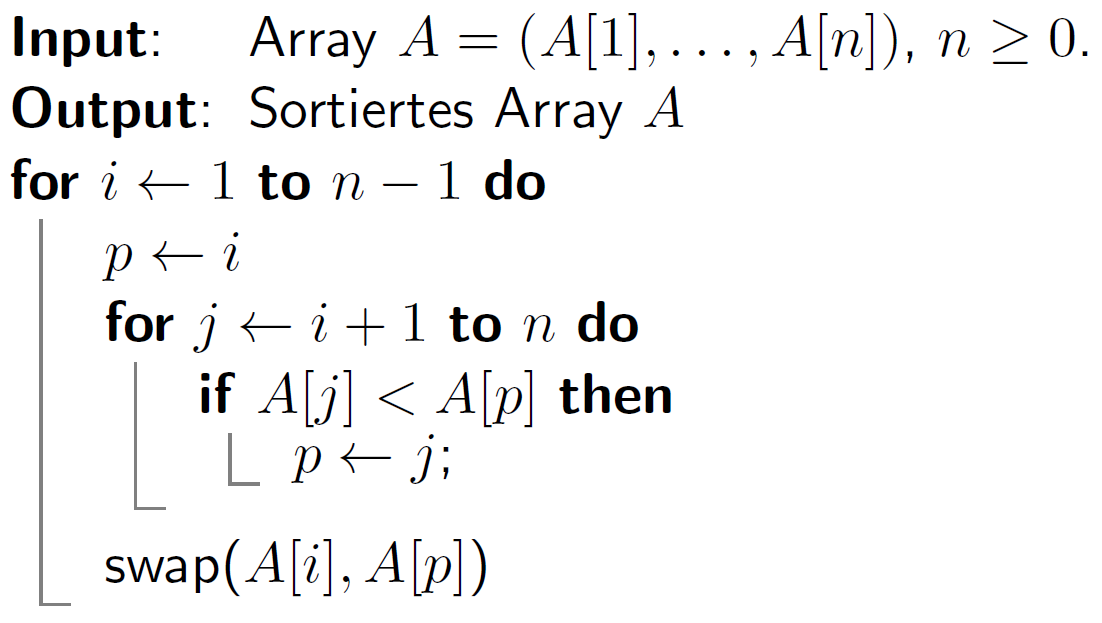
\includegraphics[width = 0.7\columnwidth]{../img/selectSortCode.png}\par\smallskip

\textbf{Analyse}\par
\begin{tabular*}{\columnwidth}{@{\extracolsep\fill}ll@{}}
Anzahl Vergleiche im schlechtesten Fall: & $\Theta(n^{2})$ \\
Anzahl Vertauschungen im schlechtesten Fall: & $n-1=\Theta(n)$\\
\end{tabular*}
\end{sectionbox}

\begin{sectionbox}
\subsection{Sortieren durch Einfügen}\smallskip
\begin{tabular*}{\columnwidth}{@{\extracolsep\fill}ll@{}}
\multirow{7}{*}{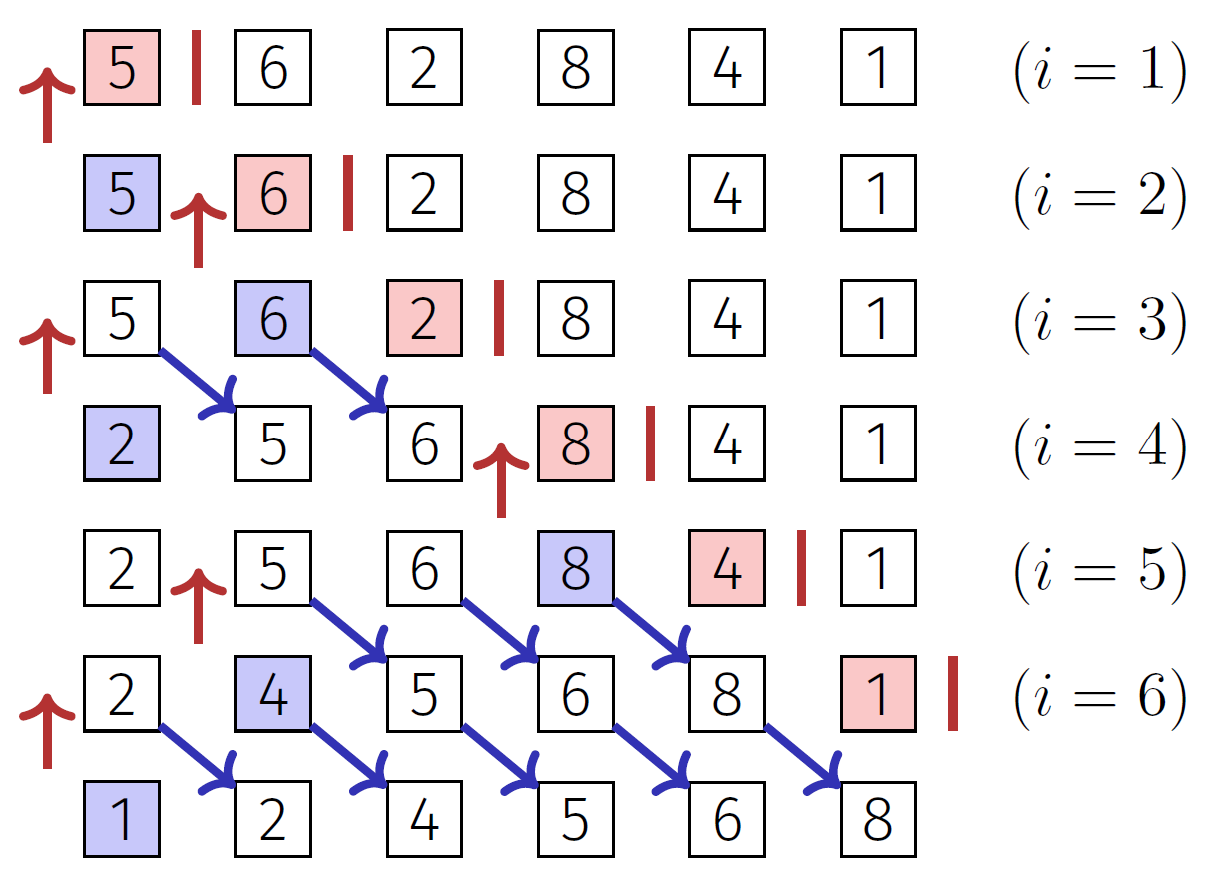
\includegraphics[width = 0.55\columnwidth]{../img/InsSort.png}}
& Iteratives Vorgehen: \\
& $i=1\rightarrow n$ \smallskip \\
& Einfügeposition für \\
& Element $i$ bestimmen. \smallskip\\
& Element $i$ einfügen, ggfs.\\
& Verschiebung nötig. \smallskip\\
& \\
& \\
\end{tabular*}\smallskip

\textbf{Selection Sort}\par
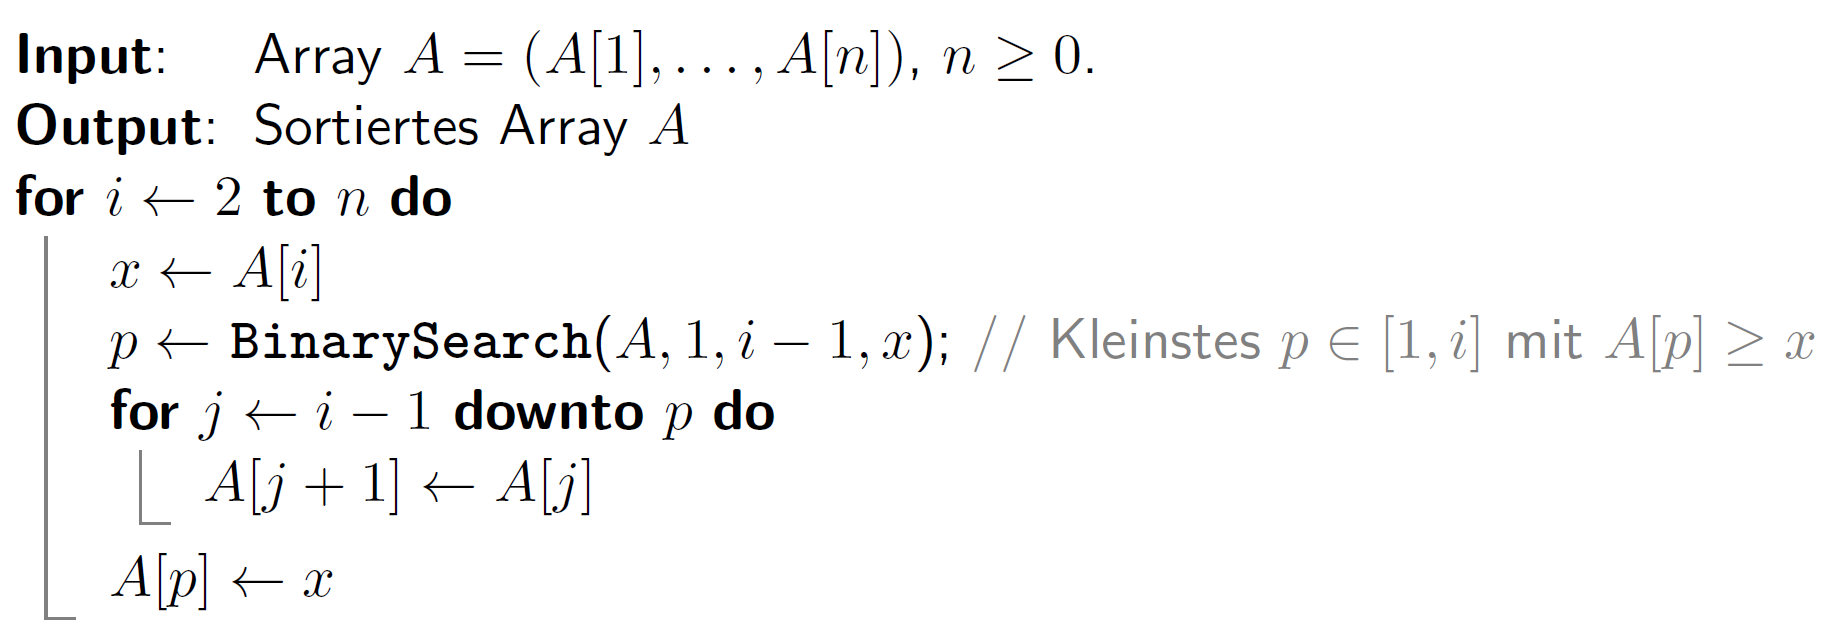
\includegraphics[width = \columnwidth]{../img/InsSortCode.png}\par\smallskip

\textbf{Analyse}\par
Nachteil: Im schlechtesten Fall viele Elementverschiebungen. / Vorteil:  Der Suchbereich (Einfügebereich) ist bereits sortiert $\rightarrow$ binäre Suche möglich.

\end{sectionbox}

\begin{sectionbox}
\subsection{Mergesort}\smallskip
\subsubsection{Merge}\smallskip
Minimum von A kann mit 2 Vergleichen ermittelt werden.\par
\begin{center}
    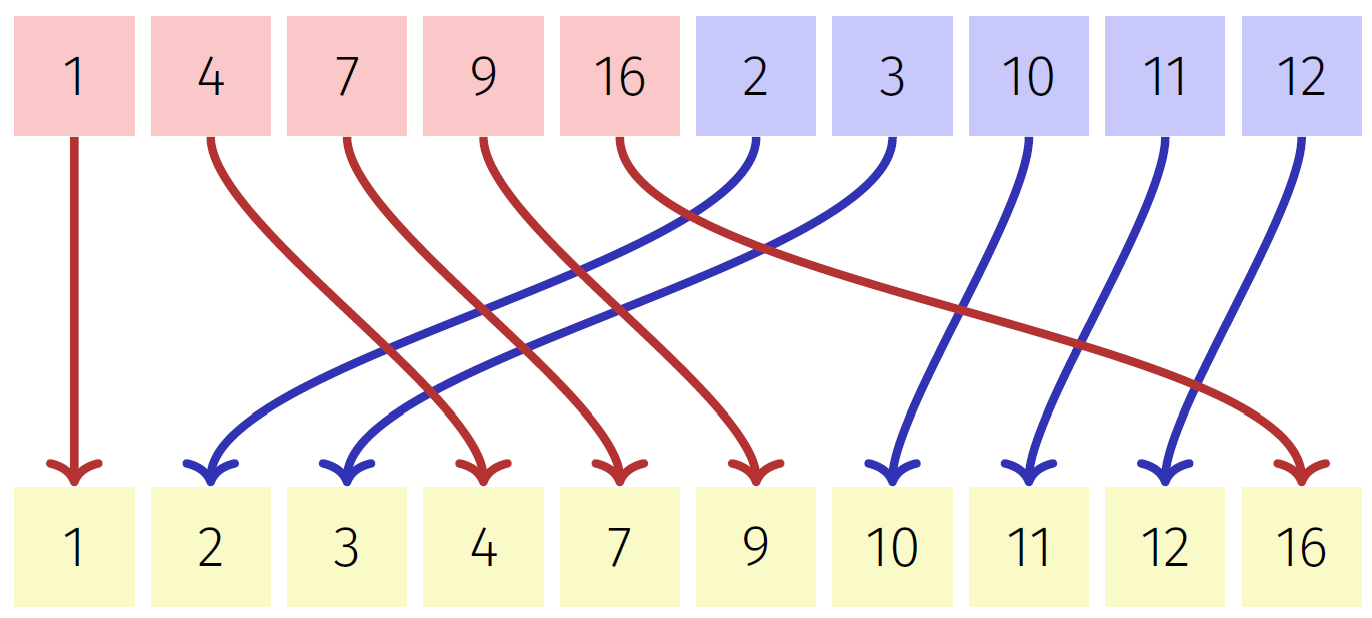
\includegraphics[width = 0.5\columnwidth]{../img/Merge.png}
\end{center}\smallskip
\textbf{Merge(A,l,m,r)}\par
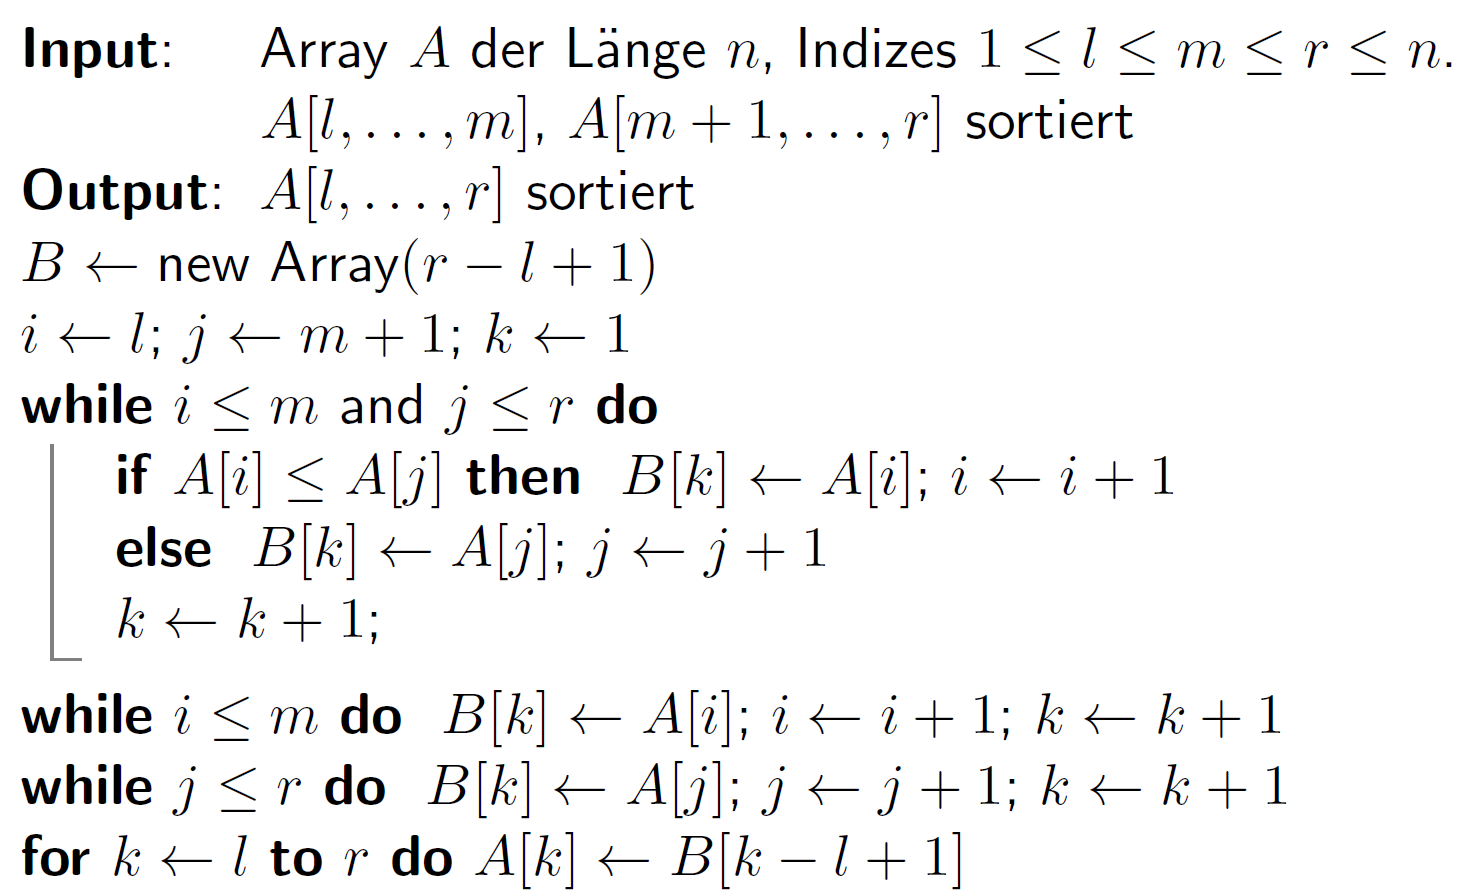
\includegraphics[width = 0.75\columnwidth]{../img/MergeCode.png}
\smallskip

\subsubsection{Mergesort}
\begin{center}
    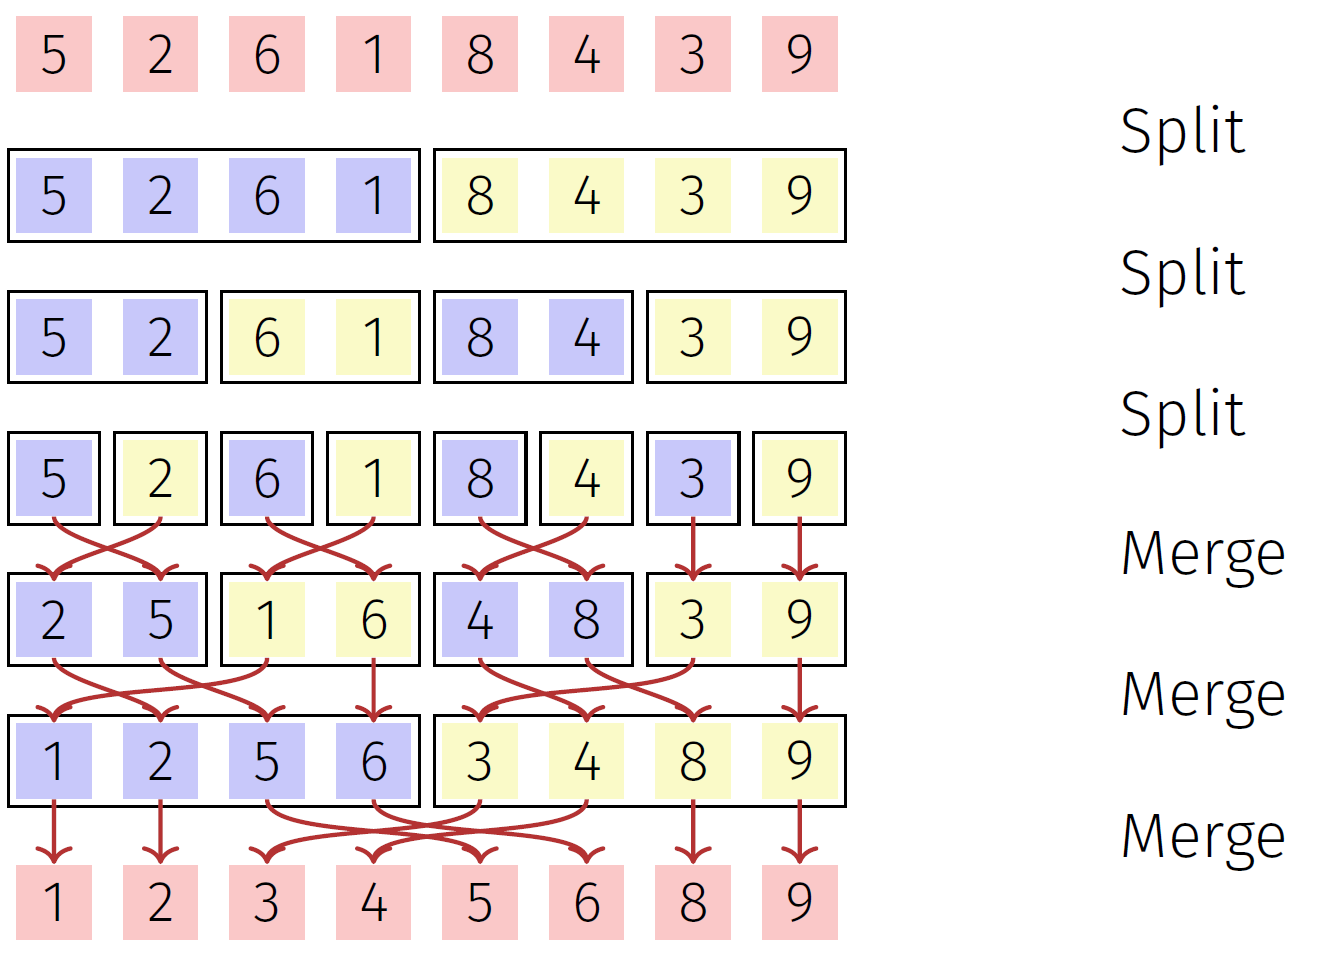
\includegraphics[width = 0.5\columnwidth]{../img/Mergesort.png}
\end{center}\smallskip
\textbf{Mergesort(A,l,r) $\rightarrow$ rekursive Variante}\par
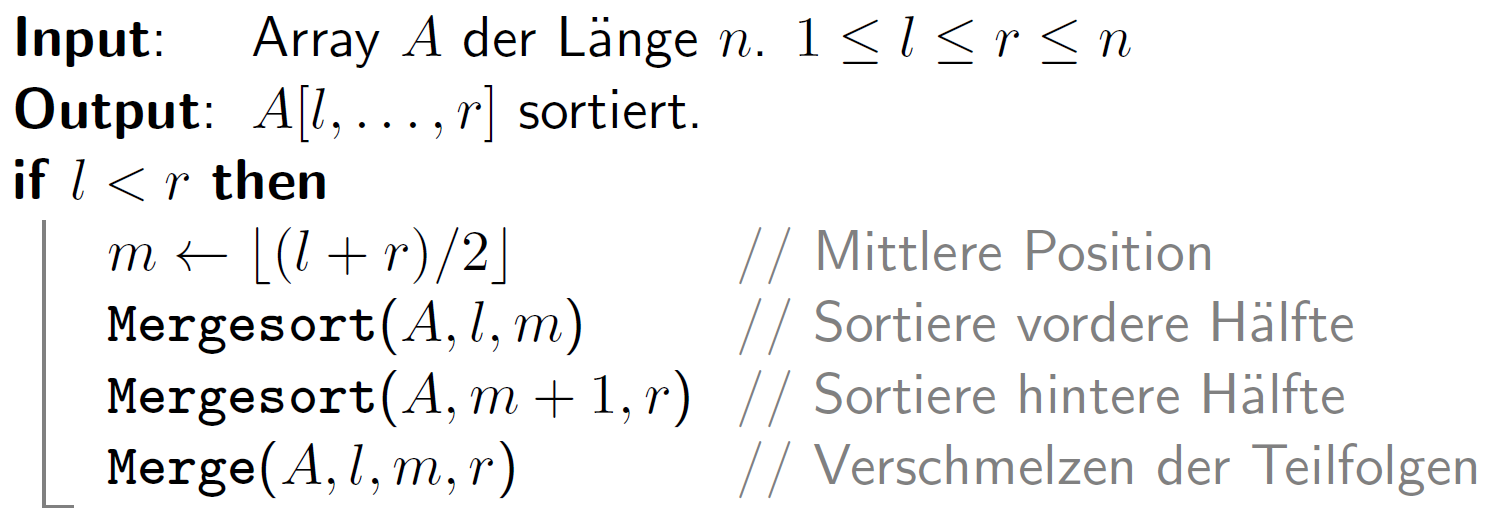
\includegraphics[width = 0.75\columnwidth]{../img/MergesortCode.png}
\par\smallskip
\textbf{Analyse}: Laufzeit  $\Theta(n \operatorname{log}(n))$
\end{sectionbox}

\begin{sectionbox}
\subsection{Quicksort}\smallskip
\textbf{Pivotieren}\par
\begin{enumerate}
    \item Wähle ein beliebiges ELement als Pivot\par
    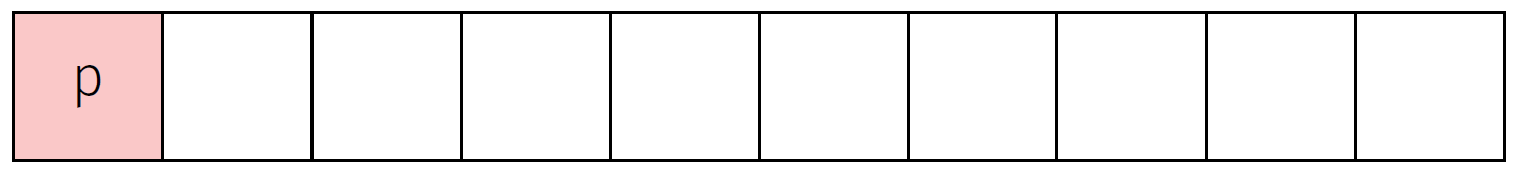
\includegraphics[width = 0.4\columnwidth]{../img/pivot1.png}
    \item Teile A in zwei Teile\par
    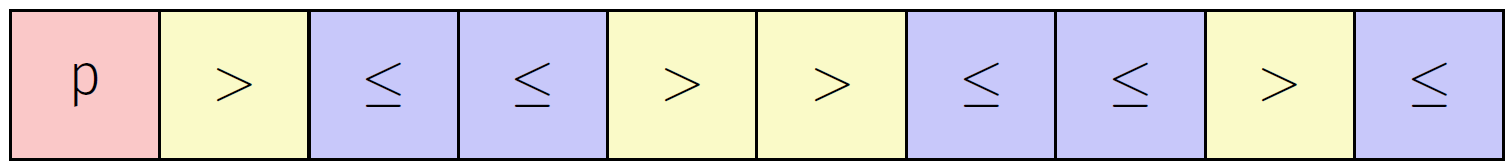
\includegraphics[width = 0.4\columnwidth]{../img/pivot2.png}
    \item Quicksort: Rekursion auf L und R\par
    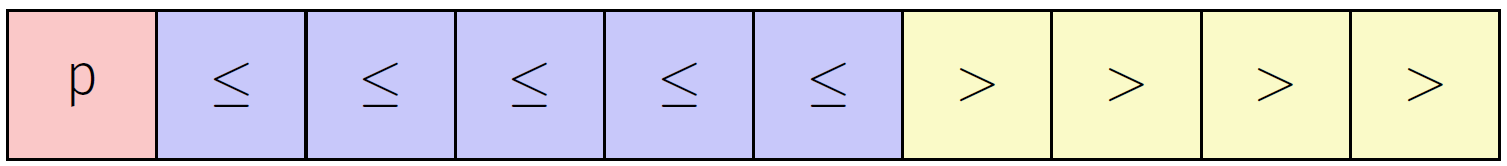
\includegraphics[width = 0.4\columnwidth]{../img/pivot3.png}
    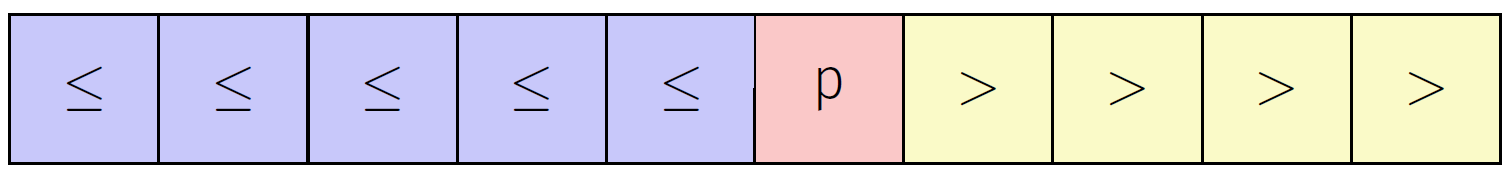
\includegraphics[width = 0.4\columnwidth]{../img/pivot4.png}
\end{enumerate}\smallskip
\textbf{Wahl des Pivot}\par
Maximum/Minimum (worst case) in $\mathcal{O}(n^{2})$.\par
Best case (Pivot in der Mitte) $\omega(n)$.\par\smallskip
\textbf{Partition(A,l,r,p)}\par
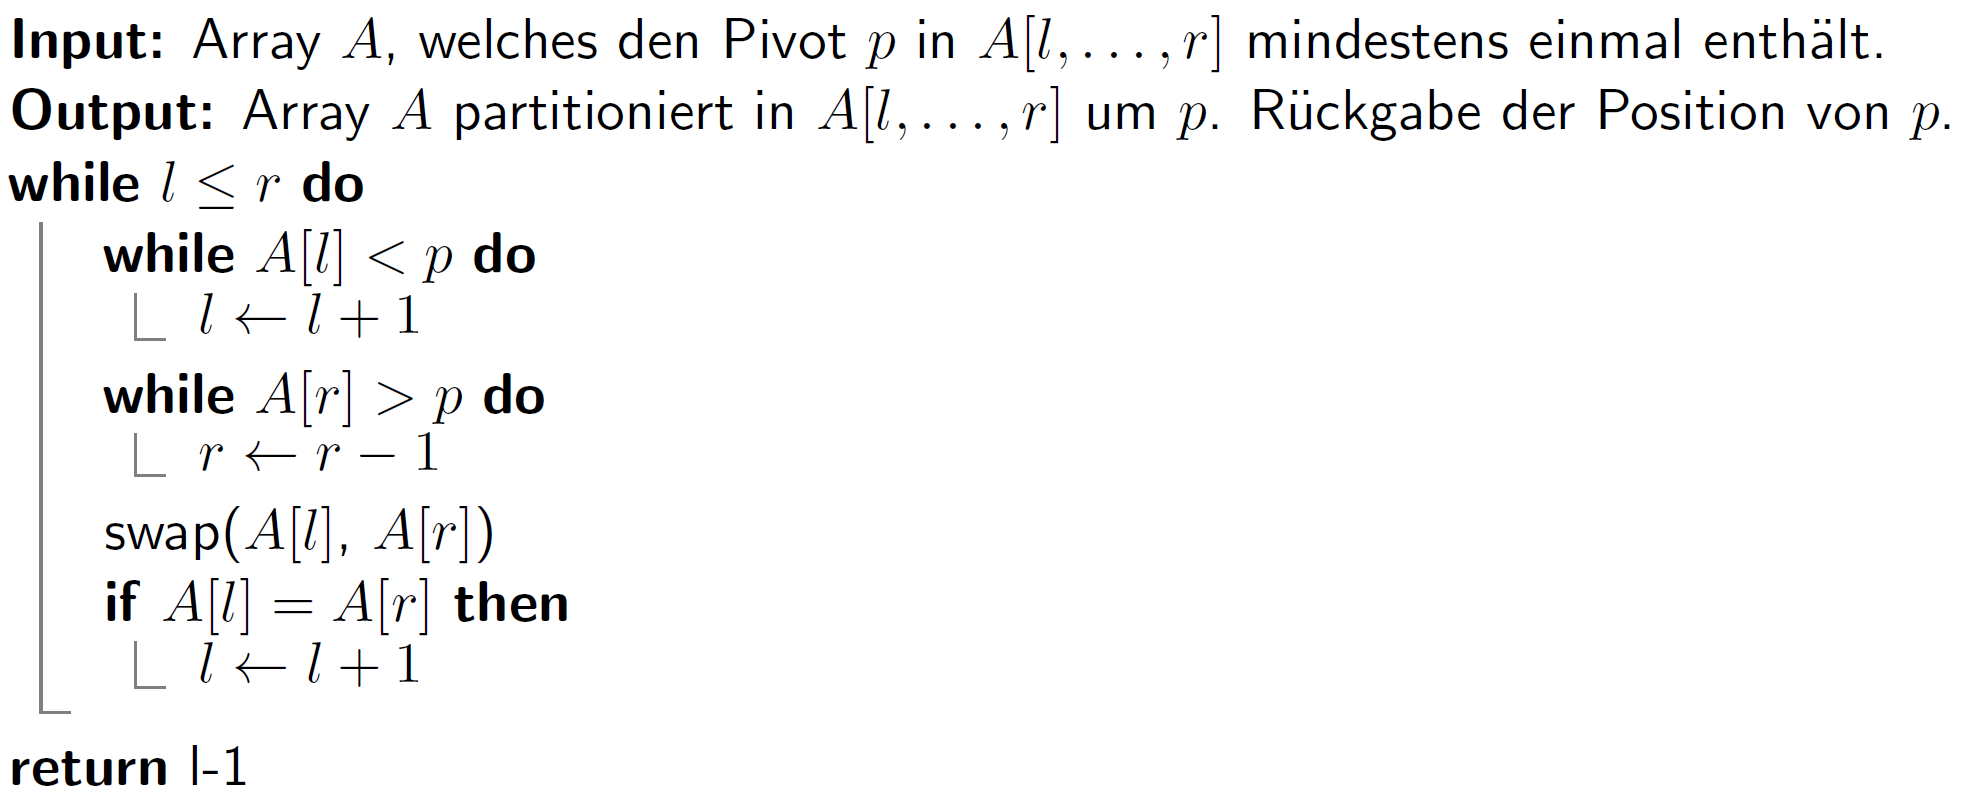
\includegraphics[width = \columnwidth]{../img/PartCode.png}
\par\smallskip

\textbf{Quicksort(A,l,r)}\par
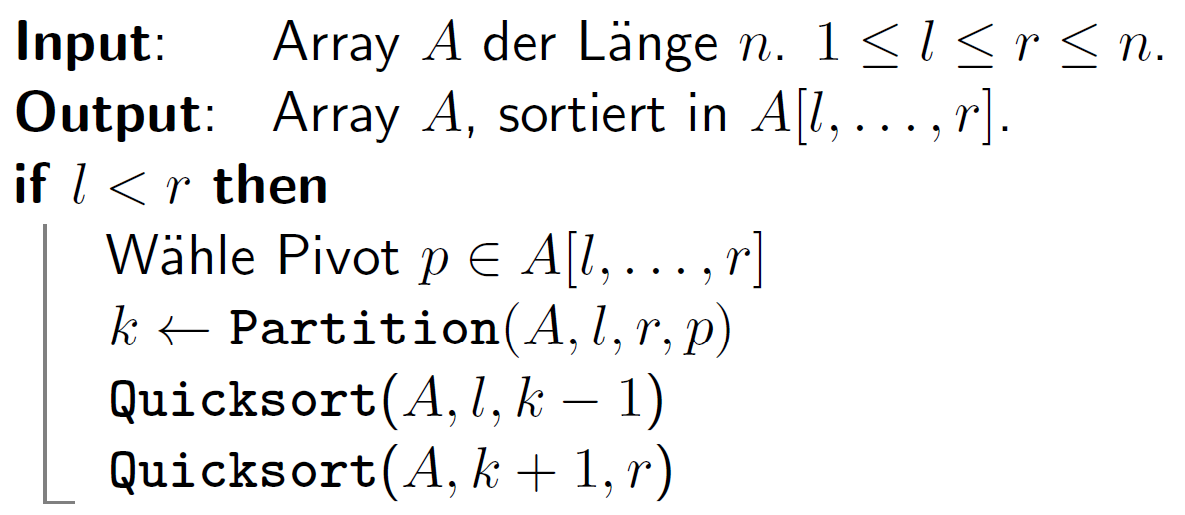
\includegraphics[width = 0.8\columnwidth]{../img/QuicksortCode.png}
\par\smallskip
\begin{greenbox}
Im Mittel benötigt randomisiertes Quicksort $\mathcal{O}(n \cdot \operatorname{log}(n))$ Vergleiche.
\end{greenbox}
\end{sectionbox}

\vspace{36px}

% SECTION ====================================================================================
\vspace{-4pt}
\begin{sectionbox}
\section{Natürliche Suchbäume}
% ============================================================================================
\subsection{Nomenklatur}
\begin{center}
    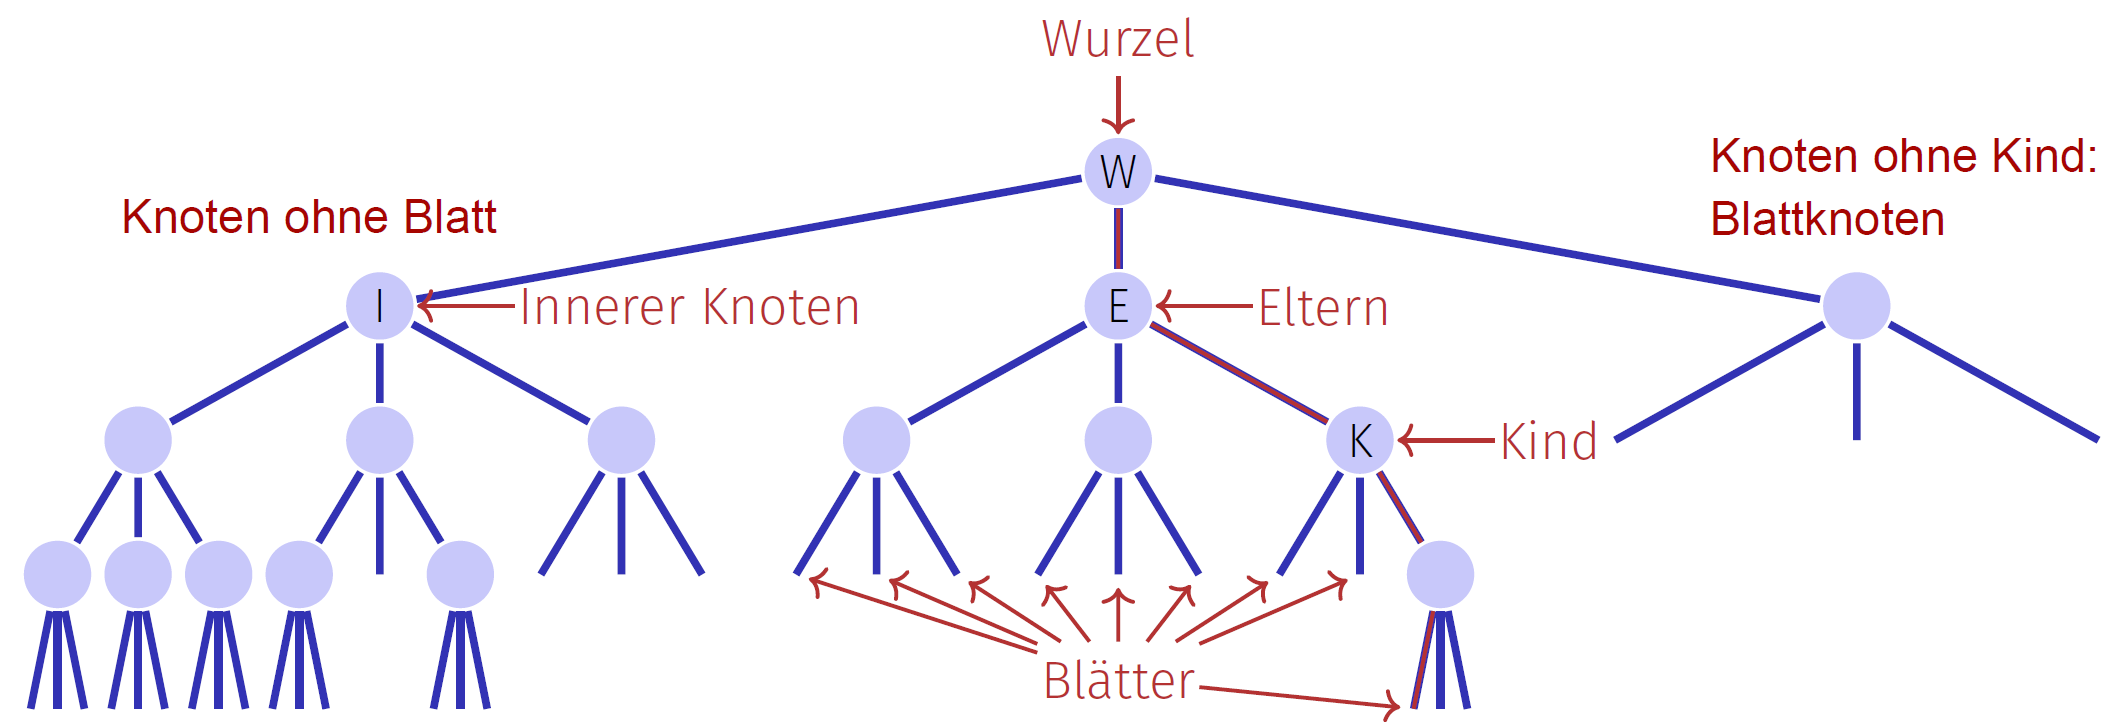
\includegraphics[width = \columnwidth]{../img/BaumNomen.png}
\end{center}
\end{sectionbox}
\vspace{-4pt}
\begin{sectionbox}
  \subsection{Binäre Suchbäume}\smallskip
  Binärer Baum (nur zwei Nachfolgerknoten) mit Eigenschaften:\par
  \begin{itemize}
      \item Jeder Knoten v speichert einen Schlüssel
      \item Schlüssel im linken Teilbaum v.left kleiner als v.key
      \item Schlüssel im rechten Teilbaum v.right grösser als v.key
  \end{itemize}\vspace{7px}
  
  \subsubsection{Höhe eines Baumes}\smallskip
  $h(r)=\left\{\begin{array}{ll}0 & \text { falls } r=\text { null } \\ 1+\max \{h(r \cdot \operatorname{left}), h(r \cdot \text { right })\} & \text { sonst. }\end{array}\right.$\par\smallskip
  Die Laufzeit der Suche ist somit im schlechtesten Fall $\mathcal{O}(h(T))$.\par\smallskip
  \end{sectionbox}
  \vspace{-4pt}
  \begin{sectionbox}
  \subsubsection{Operationen}\smallskip
  
  \textbf{Knoten entfernen}\par
  Mögliche Situationen: Knoten hat keine Kinder, Knoten hat ein Kind oder Knoten $v$ hat zwei Kinder.
  Im letzten Fall: Der kleinste Schlüssel im rechten Teilbaum $v.right$ ist der symmetrische Nachfolger von $v$ $\rightarrow$ ersetze $v$ durch seinen symmetrischen Nachfolger.
  \par Auch möglich: ersetze $v$ durch seinen symmetrischen Vorgänger
  \par Implementation: der Teufel steckt im Detail!
  \end{sectionbox}
  \vspace{-4pt}
  \begin{sectionbox}
  \textit{Grafik zu dem symmetrischen Vorgänger (links) oder Nachfolger (rechts)}\par
  \begin{center}
  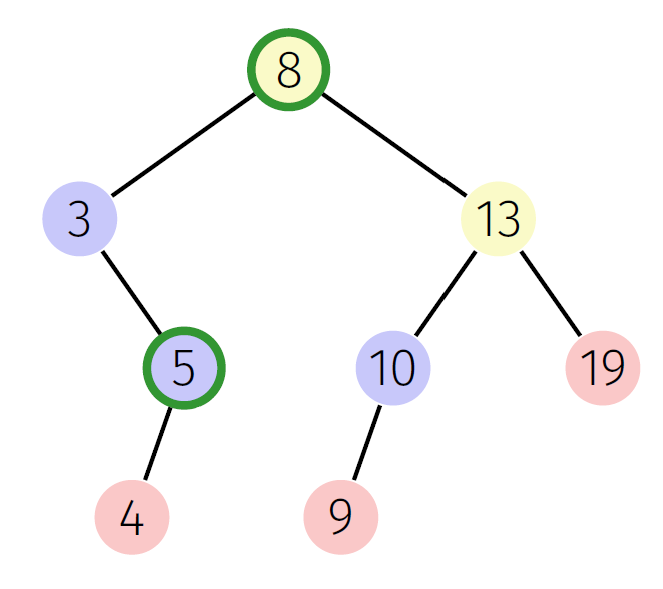
\includegraphics[width = 0.4\columnwidth]{../img/symVorg.png}
  \tab 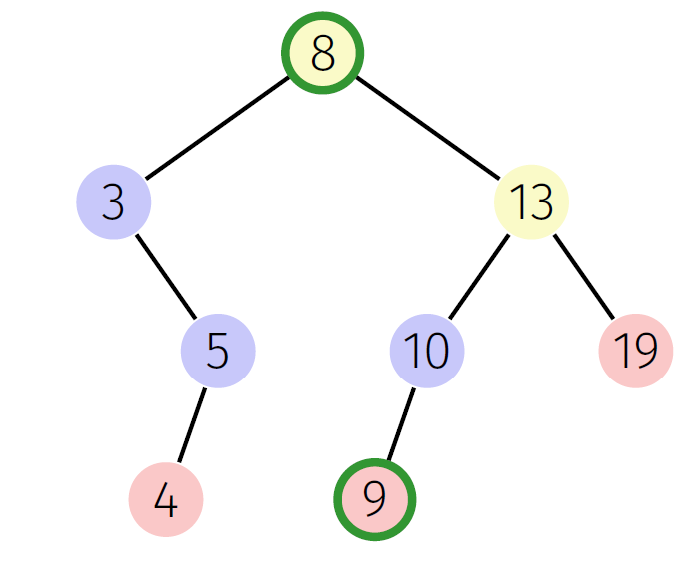
\includegraphics[width = 0.4\columnwidth]{../img/symNachf.png}    
  \end{center}
  \end{sectionbox}
  \vspace{-4pt}
  \begin{sectionbox}
  \subsection{Traversierungsarten}\smallskip
  \begin{greenbox}
  \begin{itemize}
      \item \textbf{Hauptreihenfolge} (preorder):
      \par $v$, dann $T_{left}(v)$, dann $T_{right}(v)$.
      \item \textbf{Nebenreihenfolge} (postorder):
      \par $T_{left}(v)$, dann $T_{right}(v)$, dann $v$.
      \item \textbf{Symmetrische Reihenfolge} (inorder):
      \par $T_{left}(v)$, dann $v$, dann $T_{right}(v)$.
  \end{itemize}
  \end{greenbox}\smallskip
  
  \textit{Beispiel}\par
  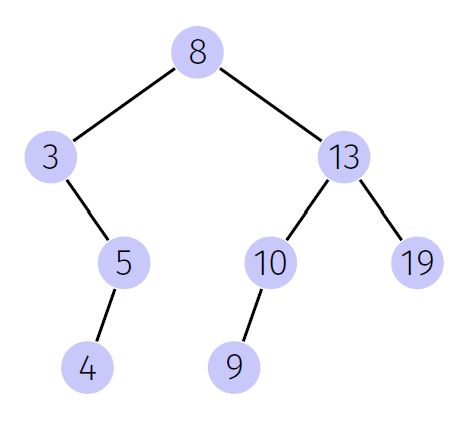
\includegraphics[width = 0.4\columnwidth]{../img/BspBST.png}
  \smallskip
  \begin{itemize}
      \item \textbf{Hauptreihenfolge} (preorder):
      \par 8, 3, 5, 4, 13, 10, 9, 19
      \item \textbf{Nebenreihenfolge} (postorder):
      \par 4, 5, 3, 9, 10, 19, 13, 8
      \item \textbf{Symmetrische Reihenfolge} (inorder):
      \par 3, 4, 5, 8, 9, 10, 13, 19
  \end{itemize}
\end{sectionbox}


\subsection{C++ - Implementation}\smallskip
\subsubsection{Tree}\smallskip
\begin{lstlisting}[language=C++]
class BST {
  Node* root;
public:
  BST();
  bool contains(int key) const;
  bool insert(int key);
  bool remove(int key);
  void print_preorder(std::ostream& out) const;
  void clear();
  ~BST();
};

// Constructor, creates an empty binary search tree
BST::BST(): root(nullptr) {}

// Returns true iff the BST contains the given key.
bool BST::contains(int key) const {
  return root == nullptr ? false : root->contains(key);
}
  
// Returns true iff the given key was inserted into the BST.
bool BST::insert(int key) {
  if (root == nullptr) {
    root = new Node(key);
    return true;
  } else {
    return root->insert(key);
  }
}
  
// Returns true iff the given key was removed from the BST.
bool BST::remove(int key) {
  if (root == nullptr) {
    return false;
  } else if (root->key == key) {
    root = Node::symmetric_successor(root);
    return true;
  } else {
    return root->remove(key);
  }
}
  
// Prints the preorder-traversal of the BST to out.
void BST::print_preorder(std::ostream& out) const {
  if (root != nullptr) {
    root->print_preorder(out);
    out << '\n';
  }
}

// Clears the BST, i.e. resets it to empty.
void BST::clear() {
  delete root;
  root = nullptr;
}

// Deconstructor
BST::~BST() {
  clear();
}
\end{lstlisting}



\subsubsection{Node}\smallskip
\begin{lstlisting}[language=C++]
struct Node {
  int key;     // Key, i.e. value stored in this node
  Node* left;  // Left child, i.e. root of left subtree
  Node* right; // Right child, i.e. root of right subtree
  
  Node(int key, Node* left, Node* right);
  
  bool contains(int search_key) const;
  bool insert(int new_key);
  bool remove(int remove_key);
  void print_preorder(std::ostream& out) const;
  static Node* symmetric_successor(Node* root);
  ~Node();
};

// Node constructor
Node::Node(int key, Node* left, Node* right): 
        key(key), left(left), right(right) {}

// POST: Returns true iff the tree contains search_key.
bool Node::contains(int search_key) const {
  const Node* curr = this;
  
  while (curr != nullptr) {
    if (curr->key == search_key) {
      return true;
    } else if (search_key < curr->key) {
      curr = curr->left;
    } else {
      assert(search_key > curr->key);
      curr = curr->right;
    }
  }
  return false;
}

// POST: Inserts new_key into the tree, if not already 
//  present. Returns true iff new_key was inserted.
//  Maintains the binary search-tree invariant.
bool Node::insert(int new_key) {
  Node* curr = this;
  
  while (curr->key != new_key) {
    if (new_key < curr->key) {
      if (curr->left == nullptr) {
        curr->left = new Node(new_key);
        return true;
      } else {
        curr = curr->left;
      }
    } else {
      assert(new_key > curr->key);
      if (curr->right == nullptr) {
        curr->right = new Node(new_key);
        return true;
      } else {
        curr = curr->right;
      }
    }
  }
  return false;
}

// PRE:  this->key != remove_key, i.e. remove_key may be 
//  contained in this node's subtrees, but not in this node 
//  directly.
// POST: If this tree contained remove_key, then the corre-
//  sponding node was removed, replaced by its symmetric 
//  successor, and true is returned. Otherwise, nothing was 
//  changed, and false is returned. 
//  Maintains the binary search-tree invariant.
bool Node::remove(int remove_key) {
  assert(this->key != remove_key);
  
  // curr descends down the tree, while we look for the a 
  // node with remove_key.
  // curr's key itself is always different from remove_key.
  Node* curr = this;
  Node* remove_node = nullptr;
  
  while (curr != nullptr && remove_node == nullptr) {
    if (
      curr->left != nullptr&& curr->left->key == remove_key){
      // curr's left child holds remove_key, and is replaced 
      // with its symmetric successor.
      remove_node = curr->left;
      curr->left = symmetric_successor(curr->left);
    } else if (
      curr->right != nullptr && 
      curr->right->key == remove_key) {
      // Analogously, for curr's right child
      remove_node = curr->right;
      curr->right = symmetric_successor(curr->right);
    } else if (remove_key < curr->key) {
      // Descend left
      curr = curr->left;
    } else {
      // Descend right
      assert(remove_key > curr->key);
      curr = curr->right;
    }
  }
  
  if (remove_node != nullptr) {
    // To prevent memory leaks, the removed node is freed
    remove_node->left = nullptr;
    remove_node->right = nullptr;
    delete remove_node;
    return true;
  } else {
    return false;
  }
}

// POST: Prints the tree's keys in preorder traversal to out.
void Node::print_preorder(std::ostream& out) const {
  out << key << ' ';
  if (left != nullptr) left->print_preorder(out);
  if (right != nullptr) right->print_preorder(out);
}

// PRE:  root != nullptr 
// POST: Returns the symmetric successor of the given root
//  node. If the symmetric successor is not a direct child of 
//  the given root, then the symmetric successor is also 
//  removed from its context, i.e. from the subtree of root 
//  where the symmetric successor was found.
Node* Node::symmetric_successor(Node* root) {
  assert(root != nullptr);
  
  // If there's at most one child node, it must be the 
  // symmetric successor, and we're done right away.
  if (root->left == nullptr) return root->right;
  if (root->right == nullptr) return root->left;

  // Otherwise, the symmetric successor must be the left-most 
  // element of root's right subtree. We use curr to descend 
  // down the tree, and parent will have parent->left == curr 
  // (if parent != nullptr). parent needed for removing the 
  // eventually found symmetric successor from its context.
  Node* curr = root->right;
  Node* parent = nullptr;
  
  // Descend leftwards. After the loop, curr is the symmetric 
  // successor.
  while (curr->left != nullptr) {
    parent = curr;
    curr = curr->left;
  }

  // Remove the symmetric successor from its context, if 
  // necessary.
  if (parent != nullptr) {
    parent->left = curr->right;
    curr->right = root->right;
  }

  curr->left = root->left;
  return curr;
}

// Deconstructor. All transitive children are recursively 
// deleted. 
Node::~Node() {
  delete left;
  delete right;
}
\end{lstlisting}


% SECTION ====================================================================================
\section{Heaps}
% ============================================================================================

\begin{sectionbox}
\subsection{[Max-]Heap}\smallskip
Datenstruktur optimiert zum schnellen Extrahieren von Minimum oder Maximum und Sortieren.\par\smallskip

Binärer Baum mit folgenden Eigenschaften\par
\begin{enumerate}
    \item Vollständig, bis auf die letzte Ebene
    \item Lücken des Baumes in der letzten Ebene höchstens rechts.
    \item \textbf{Heap-Bedingung}:
    \par Max-(Min-)Heap: Schlüssel eines Kindes kleiner (grösser) als der des Elternknotens
\end{enumerate}\smallskip

Baum $\rightarrow$ Array:
\begin{enumerate}
    \item Kinder $(i)=\{2 i, 2 i+1\}$
    \item Elter $(i)=\lfloor i / 2\rfloor$
\end{enumerate}\smallskip

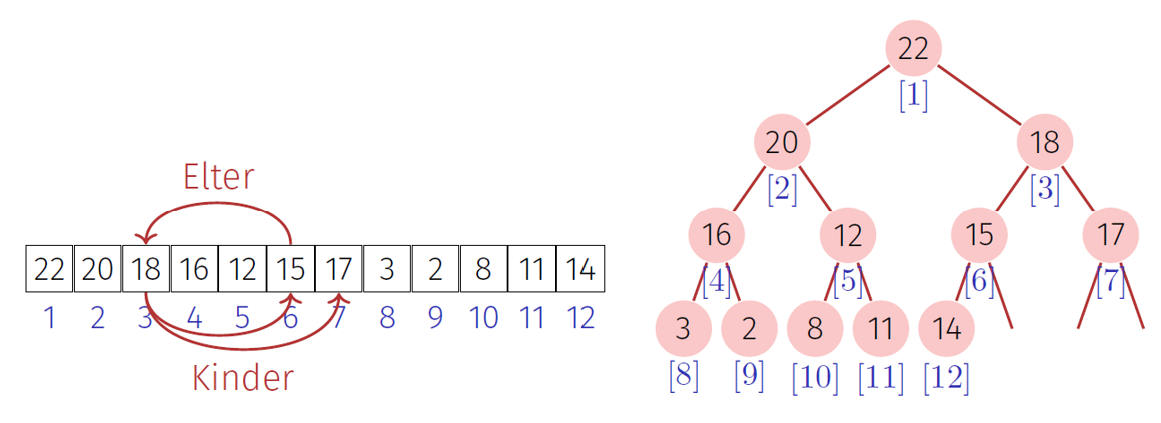
\includegraphics[width = \columnwidth]{../img/heaps.png}\smallskip

\textbf{Höhe eines Heaps}: $H(n)=\left\lceil\log _{2}(n+1)\right\rceil$\par\smallskip

\end{sectionbox}

\begin{sectionbox}
\subsection{Einfügen}\smallskip
\begin{itemize}
    \item Füge neues Element an erste freie Stelle ein.
    \item Stelle Heap Eigenschaft wieder her: \textbf{Sukzessives Aufsteigen}
    \item Anzahl Operationen im worst case: $\mathcal{O}(\operatorname{log}(n))$
\end{itemize}\smallskip
\textbf{Aufsteigen(A,m)}\par
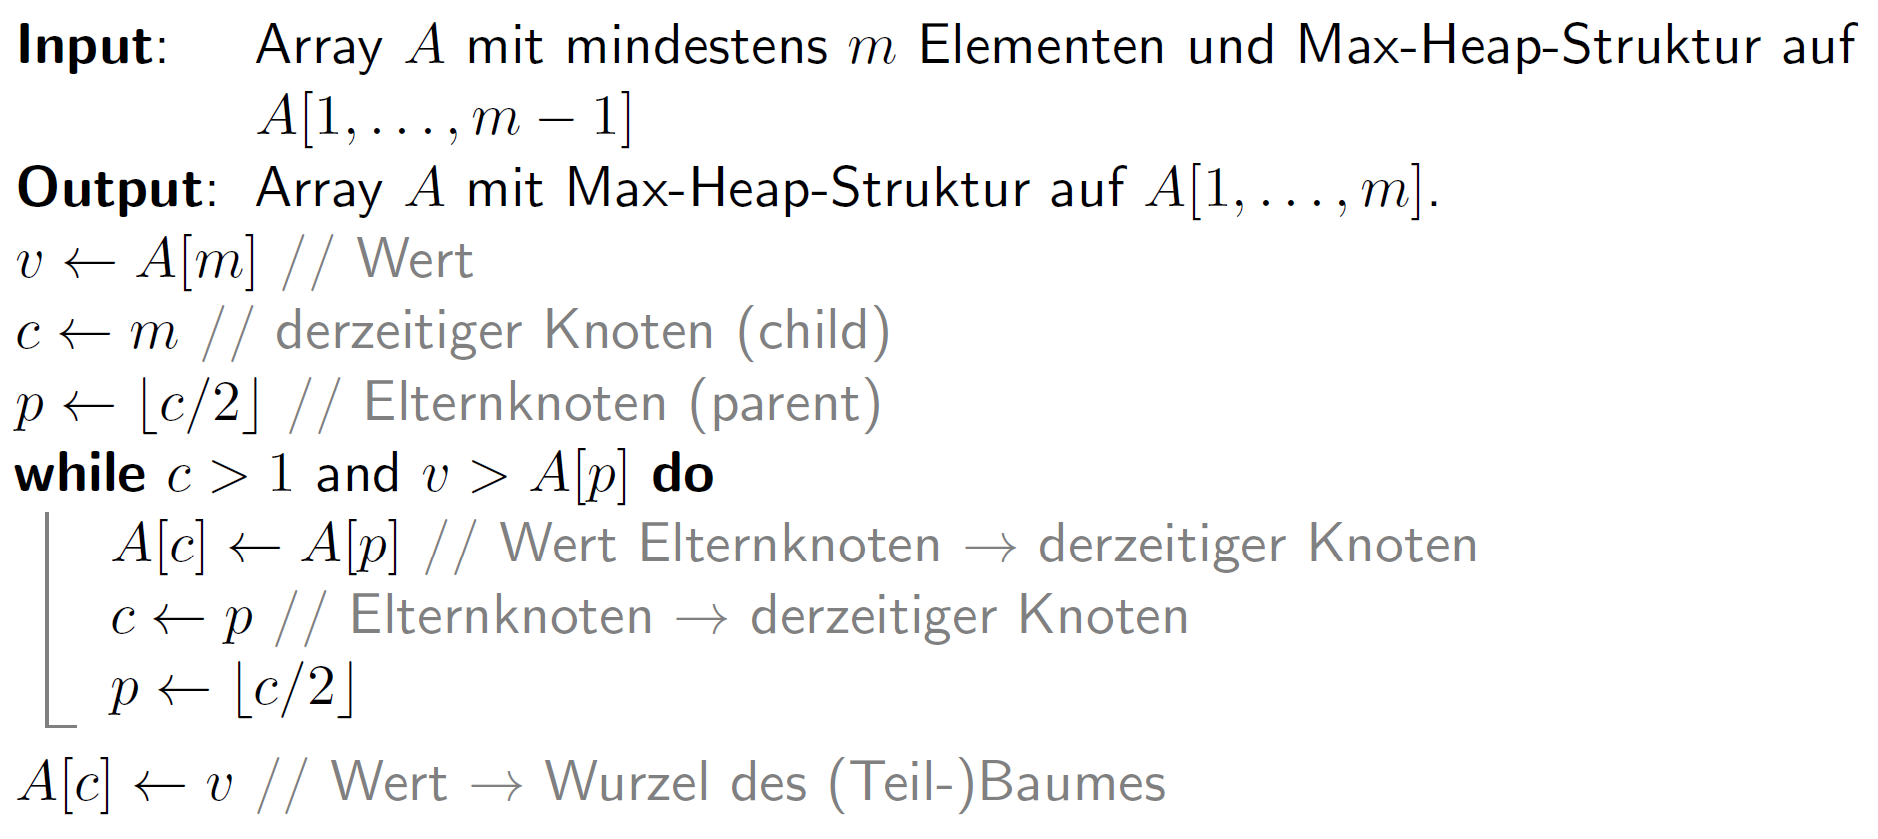
\includegraphics[width = \columnwidth]{../img/Aufsteigen.png}
\end{sectionbox}

\begin{sectionbox}
\subsection{Maximum entfernen}\smallskip
\begin{itemize}
    \item Ersetze das Maximum durch das unterste rechte Element.
    \item Stelle Heap Eigenschaft wieder her: \textbf{Sukzessives Absinken} (in Richtung des grösseren Kindes / "Max. aufsteigen lassen")
    \item Anzahl Operationen im worst case: $\mathcal{O}(\operatorname{log}(n))$
\end{itemize}\smallskip
\textbf{Versickern(A,i,m)}\par
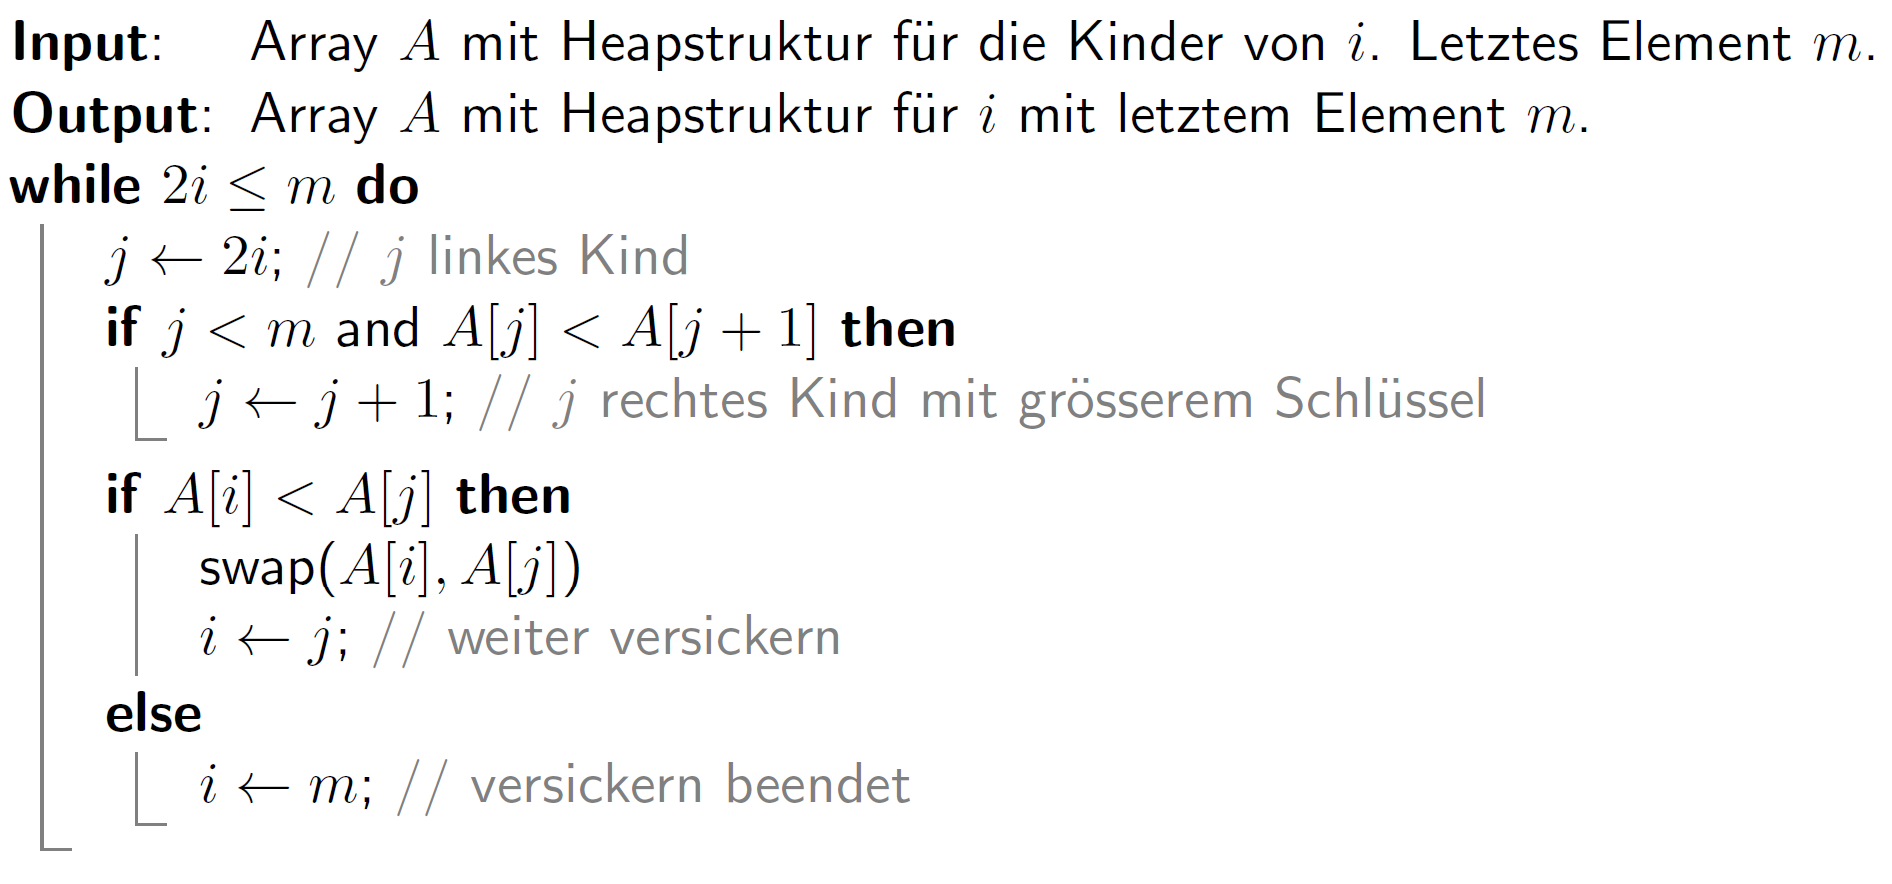
\includegraphics[width = \columnwidth]{../img/Versickern.png}
\end{sectionbox}

\begin{sectionbox}
\subsection{Heap sortieren}\smallskip
\begin{itemize}
    \item Extrahiere Maximum, stelle es hinten hin
    \item Stelle Heap Eigenschaft wieder her
    \item Wiederhole
    \item Worst case: $\mathcal{O}(n \cdot \operatorname{log}(n))$
\end{itemize}

\begin{lstlisting}[language=Python]
class HeapSort(object):

    def swap(self, list_a, i, j):
      list_a[i], list_a[j] = list_a[j], list_a[i]

    def siftDown(self, list_a, index, size):
      while(2 * index + 1 < size):
          j = 2 * index + 1
          if j + 1 < size and list_a[j] < list_a[j+1]:
              j += 1
          if list_a[index] < list_a[j]:
              self.swap(list_a,index,j)
              index = j
          else:
              return

    def heapify(self, list_a):
      n = len(list_a)
      for i in range(n//2 - 1,-1,-1):
        self.siftDown(list_a, i, n)

    def sort(self, list_a):
      n = len(list_a)
      self.heapify(list_a)
      for i in range(n-1,0,-1):
        self.swap(list_a, 0, i)
        self.siftDown(list_a, 0, i)
\end{lstlisting}\vspace{-4px}
\end{sectionbox}

\begin{sectionbox}
\subsection{Heap bauen}\smallskip
\begin{itemize}
    \item Jedes Blatt eines Heaps ist für sich schon ein korrekter Heap. $\rightarrow$ Induktion von unten!
    \item Aufrufe an Versickern: $n/2$. Also Anzahl Vergleiche und Bewegungen $v(n) \in \mathcal{O}(n \cdot \operatorname{log}(n))$.
    \item Versickerpfade sind aber im Mittel viel kürzer: $\mathcal{O}(n)$
\end{itemize}
\end{sectionbox}

% SECTION ====================================================================================
\section{AVL Bäume}
% ============================================================================================
\vspace{-4pt}
\begin{sectionbox}
\textbf{Ziel}: Verhinderung der Degenerierung $\rightarrow$ garantiere, dass ein Baum mit $n$ Knoten stets eine Höhe von $\mathcal{O}(\operatorname{log}(n))$.\par\smallskip
\subsection{AVL Bedingung}\smallskip
\subsubsection{Balance eines Knotens}\smallskip
Die Balance eines Knotens $v$ ist definiert als die Höhendifferenz seiner beiden Teilbäume $T_{l}(v)$ und $T_{r}(v)$:\par\smallskip
\begin{center}
    $\operatorname{bal}(v):=h\left(T_{r}(v)\right)-h\left(T_{l}(v)\right)$
\end{center}\par\smallskip
\begin{itemize}
    \item \textbf{Augmentieren}: $v.size$ Feld mit \textbf{Balance}
    \item \textbf{Baumhöhe}: Ein AVL Baum ist asymptotisch nicht mehr als 44\% höher als ein perfekt balancierter Baum ($\left\lceil\log _{2} n+1\right\rceil$).
\end{itemize}\par\smallskip

\subsubsection{AVL Bedingung}\smallskip
AVL Bedingung: für \textit{jeden} Knoten $v$ eines Baumes gilt:\par\smallskip
\begin{center}
    $\operatorname{bal}(v) \in\{-1,0,1\}$
\end{center}\par\smallskip

\textit{Beispiele}\par
\begin{center}
    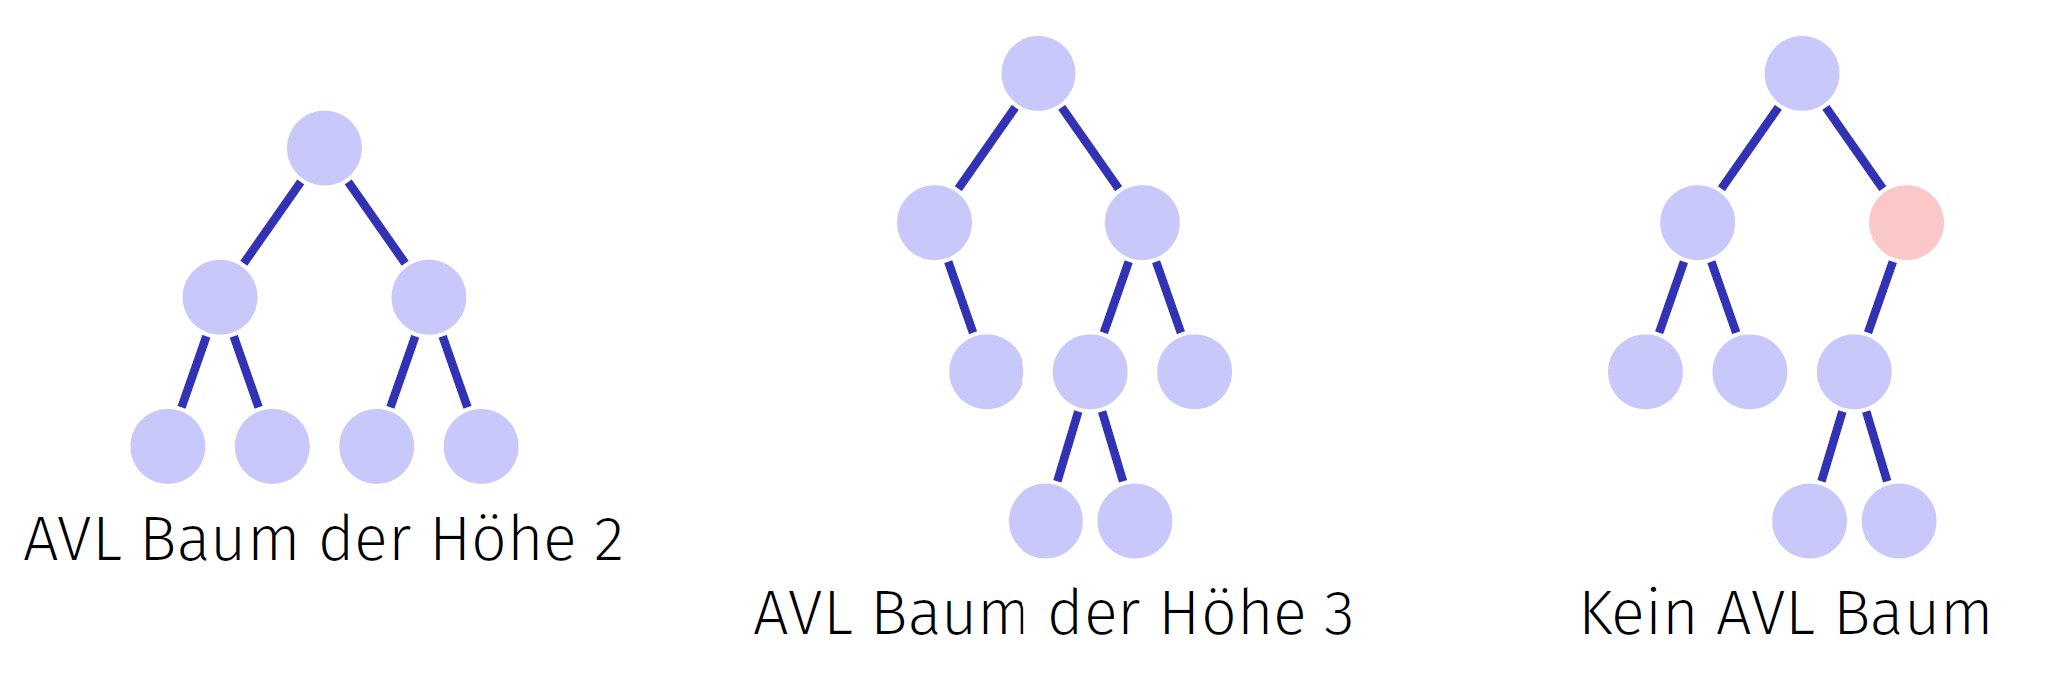
\includegraphics[width = \columnwidth]{../img/BspAVLHoehen.png}
\end{center}

\end{sectionbox}
\vspace{-4pt}
\begin{sectionbox}
\subsection{Einfügen}\smallskip
\begin{itemize}
    \item Zuerst einfügen wie bei Suchbaum.
    \item Prüfe die Balance-Bedingung für alle Knoten aufsteigend von n zur Wurzel.
    \par \textbf{$\operatorname{upin}(p)$}: Aufsteigend von $p$ die Balance (Augmentation) anpassen, wobei gilt $\operatorname{bal}(p) \in \{-1,0,+1\}$.
    \item Problematischer Fall (rebalancieren!): $p$ ist linker Sohn von $pp$, wobei $\operatorname{bal}(pp)$ bereits vor dem Einfügen $-1$ ist (danach $-2$).
\end{itemize}\par\smallskip
\end{sectionbox}
\vspace{-4pt}
\begin{sectionbox}
\subsection{Rebalancieren: Rotationen}\smallskip
\textit{Fall 1: Rotation nach rechts}\par
\begin{center}
    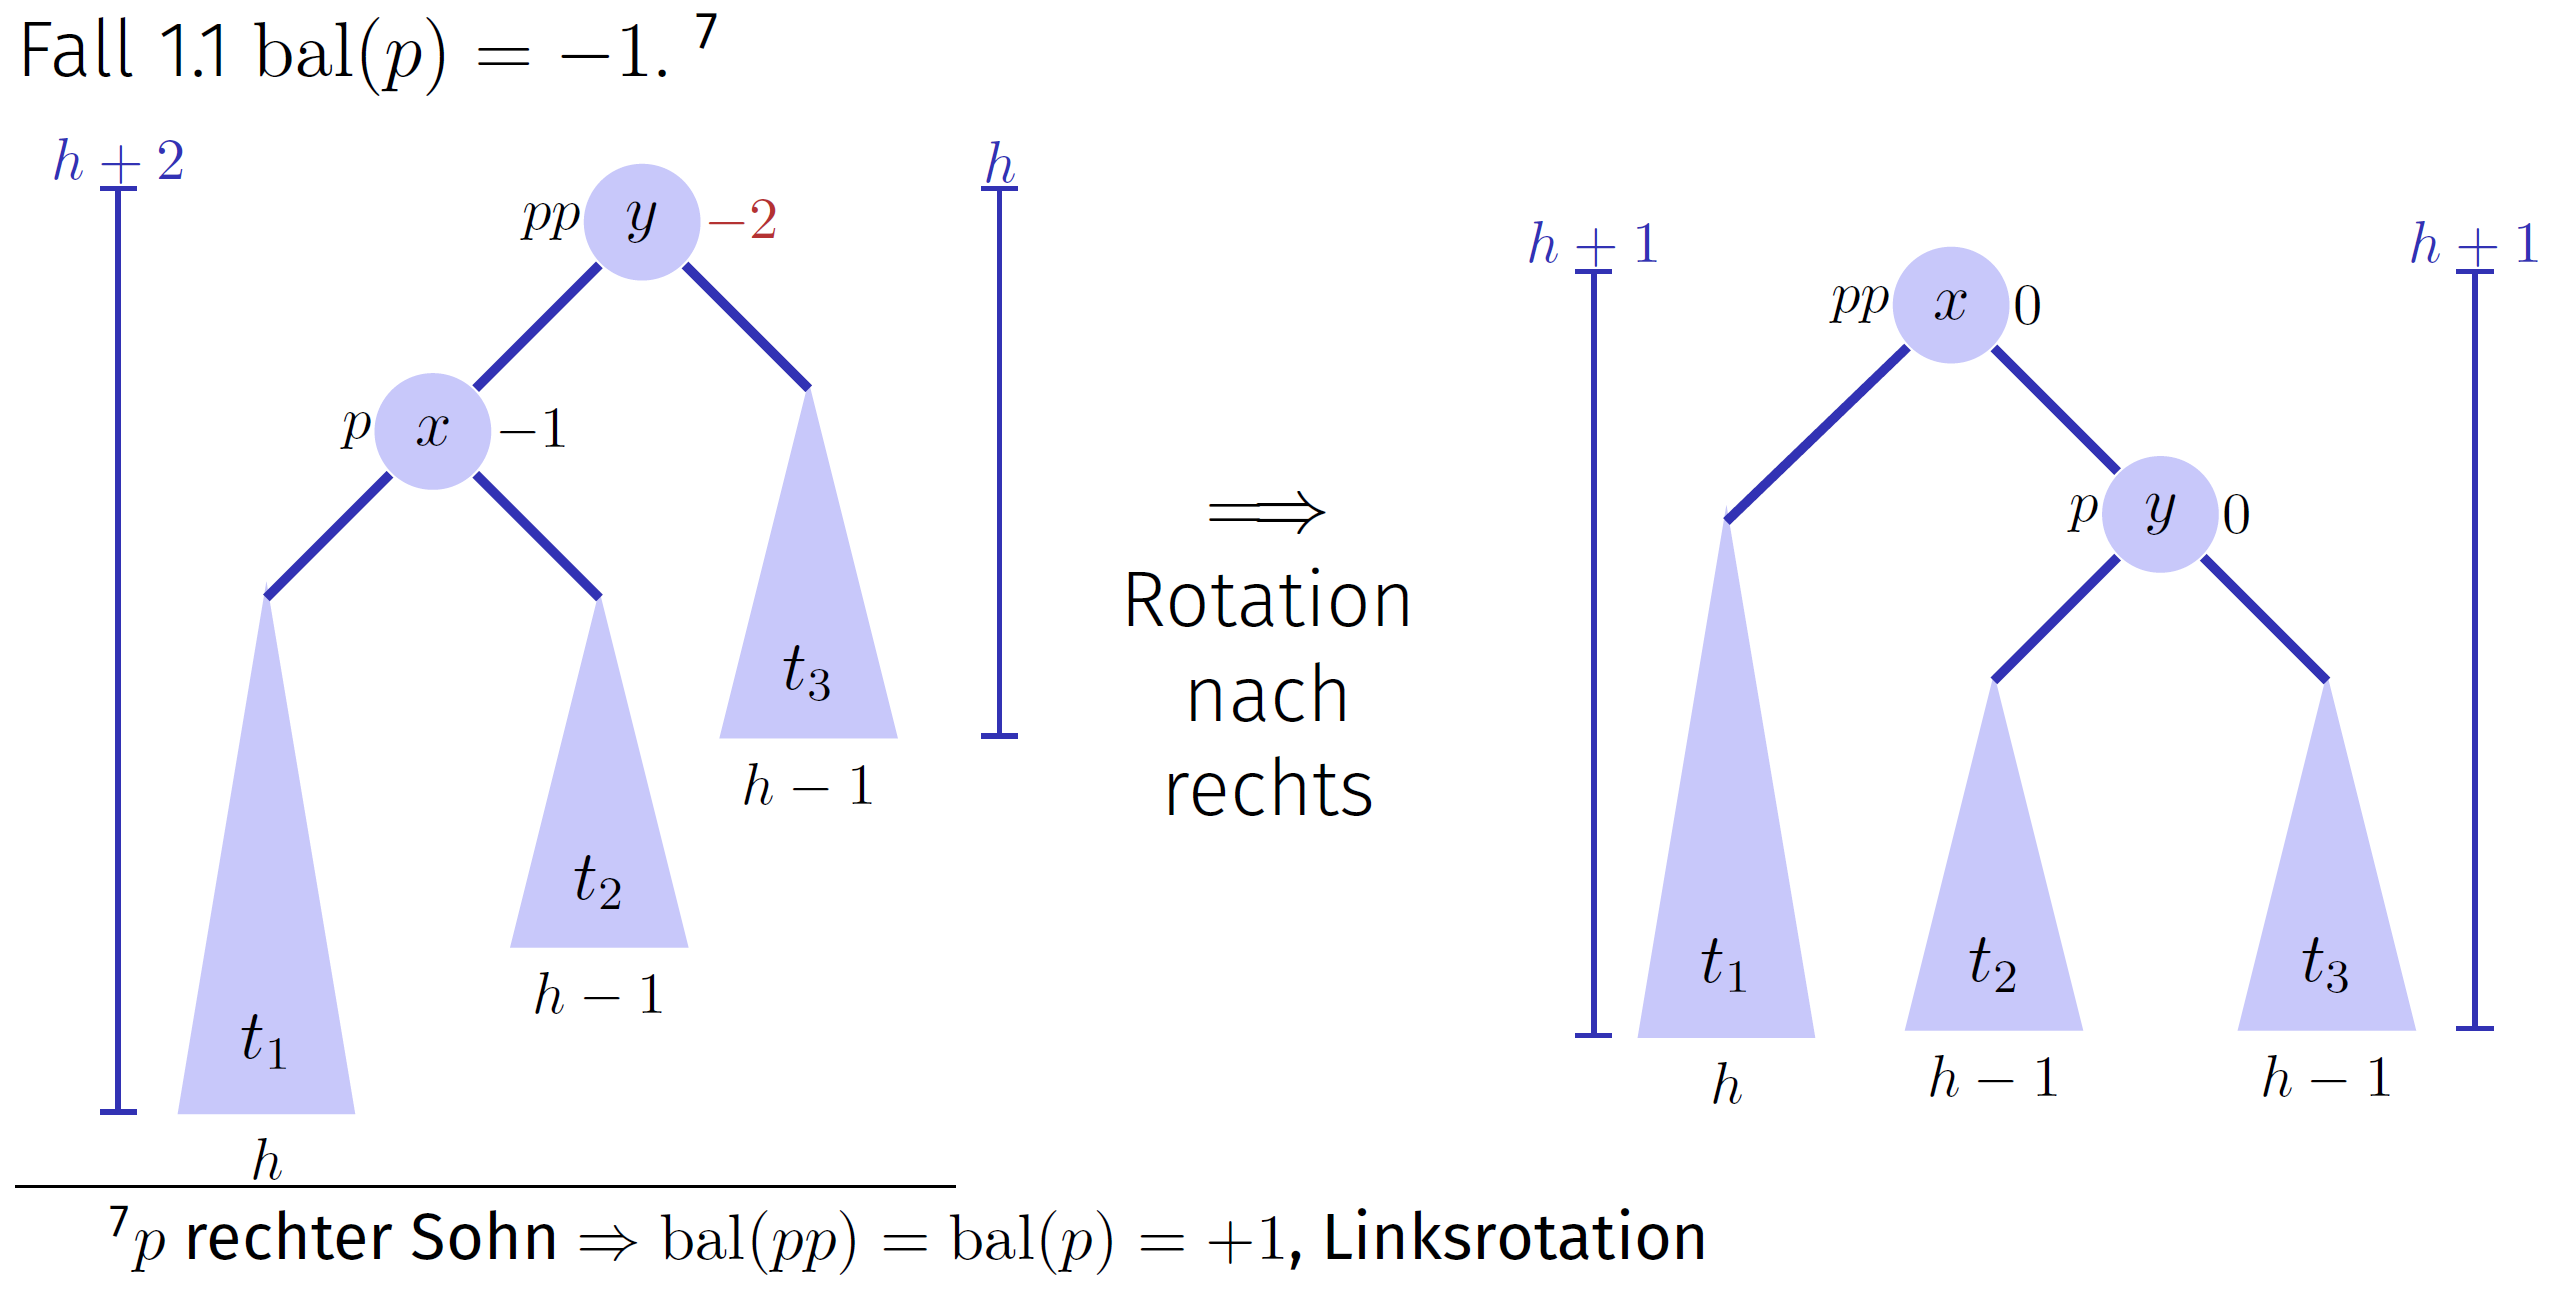
\includegraphics[width = \columnwidth]{../img/rotR.png}
\end{center}\smallskip
\end{sectionbox}
\vspace{-4pt}
\begin{sectionbox}
\textit{Fall 2: Doppelrotation nach links-rechts}\par
\begin{center}
    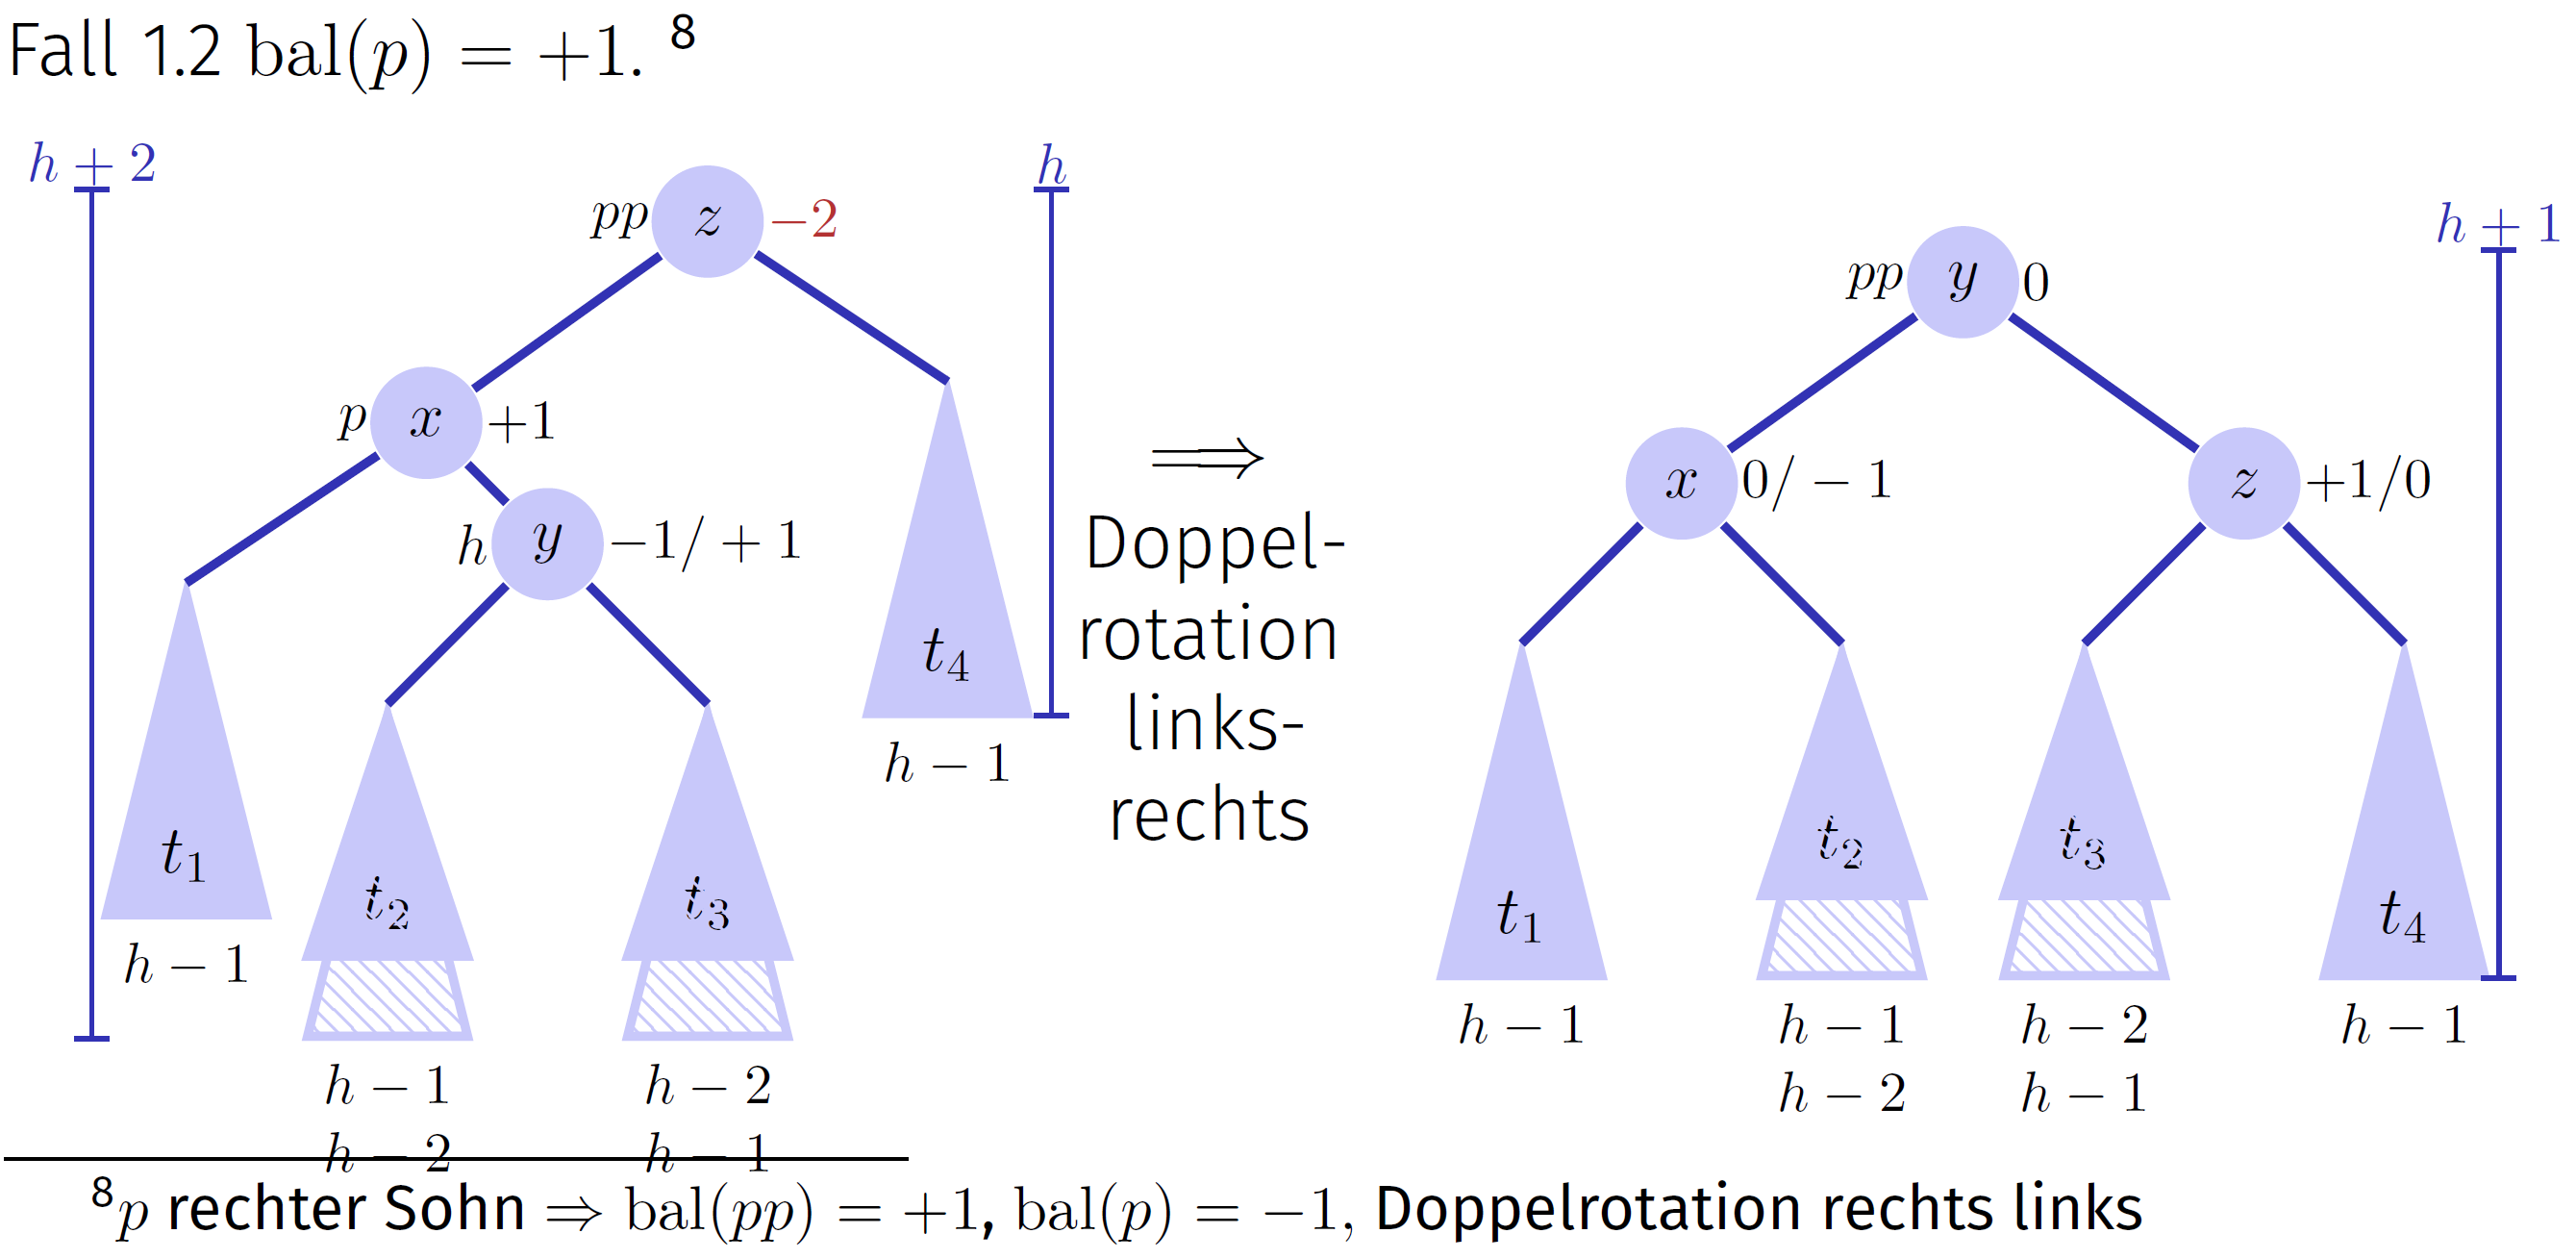
\includegraphics[width = \columnwidth]{../img/rotLR.png} \par\smallskip
    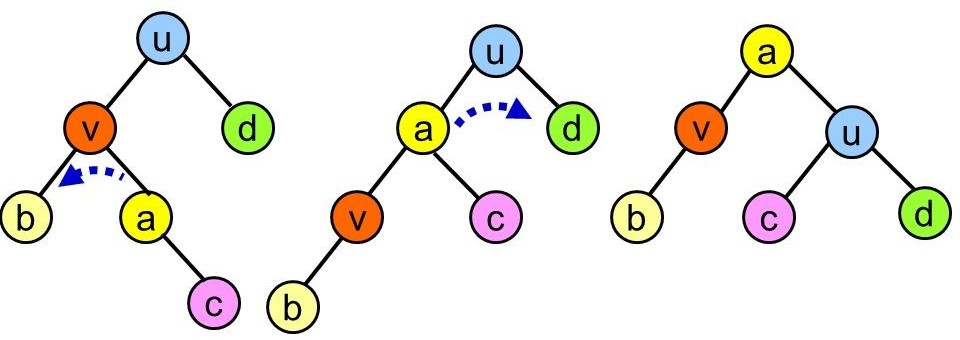
\includegraphics[width = \columnwidth]{../img/Doppelrotationen.jpg}
\end{center}\smallskip
\end{sectionbox}
\vspace{-4pt}
\begin{sectionbox}
\subsection{Analyse}\smallskip
AVL-Bäume haben asymptotische Laufzeit von $\mathcal{O}(\operatorname{log}(n))$ (schlechtester Fall) für das Suchen, Einfügen und Löschen von Schlüsseln. Einfügen und Löschen ist verhältnismässig aufwändig und für kleine Probleme relativ langsam.
\end{sectionbox}


% TODO: what is this?
% \begin{sectionbox}
% \subsection{Beispiel: Augmentierter SearchNode}\smallskip
% \begin{lstlisting}[language=Python]
% class SearchNode(object):
%   def __init__(self, k):
%     self.key = k
%     self.left = self.right = None
%     self.size = 1       # Augmentiere Hoehe mit 1
% \end{lstlisting}\vspace{-6px}
% \end{sectionbox}

% SECTION ====================================================================================
\section{Hashing}
% ============================================================================================
\vspace{-4pt}
\begin{sectionbox}
\subsection{Motivation und Idee}\smallskip
Key/Value-Paare effizient abspeichern und finden z.B. für Implementation eines Dicts oder einer Datenbank.\par\smallskip

\begin{center}
    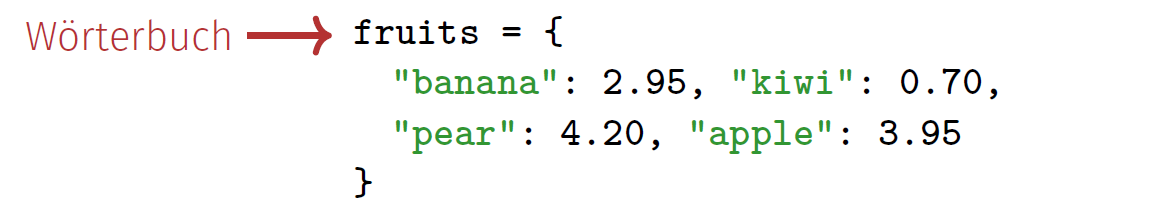
\includegraphics[width = 0.8\columnwidth]{../img/BspPreHashing.png}
\end{center}\smallskip

\textbf{Idee}\par
Direkter Zugriff (Array)\par\smallskip
\begin{greenbox}
\textbf{Probleme}\par
\begin{enumerate}
    \item \textbf{Schlüssel müssen nichtnegative ganze Zahlen sein}
    \item \textbf{Grosser Schlüsselbereich $\rightarrow$ grosses Array}
\end{enumerate}
\end{greenbox}
\end{sectionbox}
\vspace{-4pt}
\begin{sectionbox}
\subsection{Pre-Hashing: Lösung des ersten Problems}\smallskip
Prehashing: Bilde Schlüssel ab auf positive Ganzzahlen mit einer Funktion $ph: \mathcal{K} \rightarrow \mathbb{N}$\par\smallskip
\textbf{Pre-Hashing: Beispiel String}\par
Zuordnung Name $s=s_{1} s_{2} \ldots s_{l_{s}}$ zu Schlüssel\par\smallskip
\begin{center}
    $\operatorname{ph}(s)=\left(\sum_{i=0}^{l_{s}-1} s_{l_{s}-i} \cdot b^{i}\right) \bmod 2^{w}$
\end{center}\par\smallskip
$b$ so, dass verschiedene Namen möglichst verschiedene Schlüssel erhalten.
$w$ Wortgrösse des Systems (z.B. 32 oder 64).\par\smallskip
\begin{lstlisting}[language=C++]
unsigned prehash(std::string s) {
    unsigned b = B;
    unsigned h = 0;
    
    for (unsigned i = 0; i < s.size(); ++i){
        h = h * b + s[i];
    }
    return h;
}
\end{lstlisting}\vspace{-6px}
\end{sectionbox}
\vspace{-4pt}
\begin{sectionbox}
\subsection{Hashing: Lösung des zweiten Problems}\smallskip
Reduziere des Schlüsseluniversum: Abbildung (Hash-Funktion) $h: \mathcal{K} \rightarrow\{0, \ldots, m-1\}(m \approx n=\text { Anzahl Einträge in der Tabelle })$\par\vspace{7px}

\subsubsection{Nomenklatur}\par\smallskip
\textbf{Hashfunktion} $h$: Abbildung aus der Menge der Schlüssel $\mathcal{K}$ auf die Indexmenge $\{0,1, \ldots, m-1\}$ eines Arrays (\textbf{Hashtabelle})\par
Meist $|\mathcal{K}| \gg m$, Es gibt also $k_{1}, k_{2} \in \mathcal{K}$ mit $h\left(k_{1}\right)=h\left(k_{2}\right)$ (\textbf{Kollision}). Eine Hashfunktion sollte die Menge der Schlüssel möglichst gleichmässig auf die Positionen der Hashtabelle verteilen.\par\vspace{7px}

\subsubsection{Gebräuchliche Hashfunktion: Divisionsmethode}\par\smallskip
\begin{center}
    $h(k)=k \bmod m$
\end{center}
Ideal: $m$ Primzahl, nicht zu nahe bei Potenzen von 2 oder 10\par
Aber oft: $m=2^{k}-1(k \in \mathbb{N})$
\end{sectionbox}
\vspace{-4pt}
\begin{sectionbox}
\subsection{Konzept 1: Hashing mit Verkettung}\par\smallskip
Direkte Verkettung der Überläufer.\par
$\rightarrow$ Resultuiert im worst case in $\Theta(n^{2})$ pro Operation\par\smallskip

\textit{Beispiel}\par
\begin{center}
    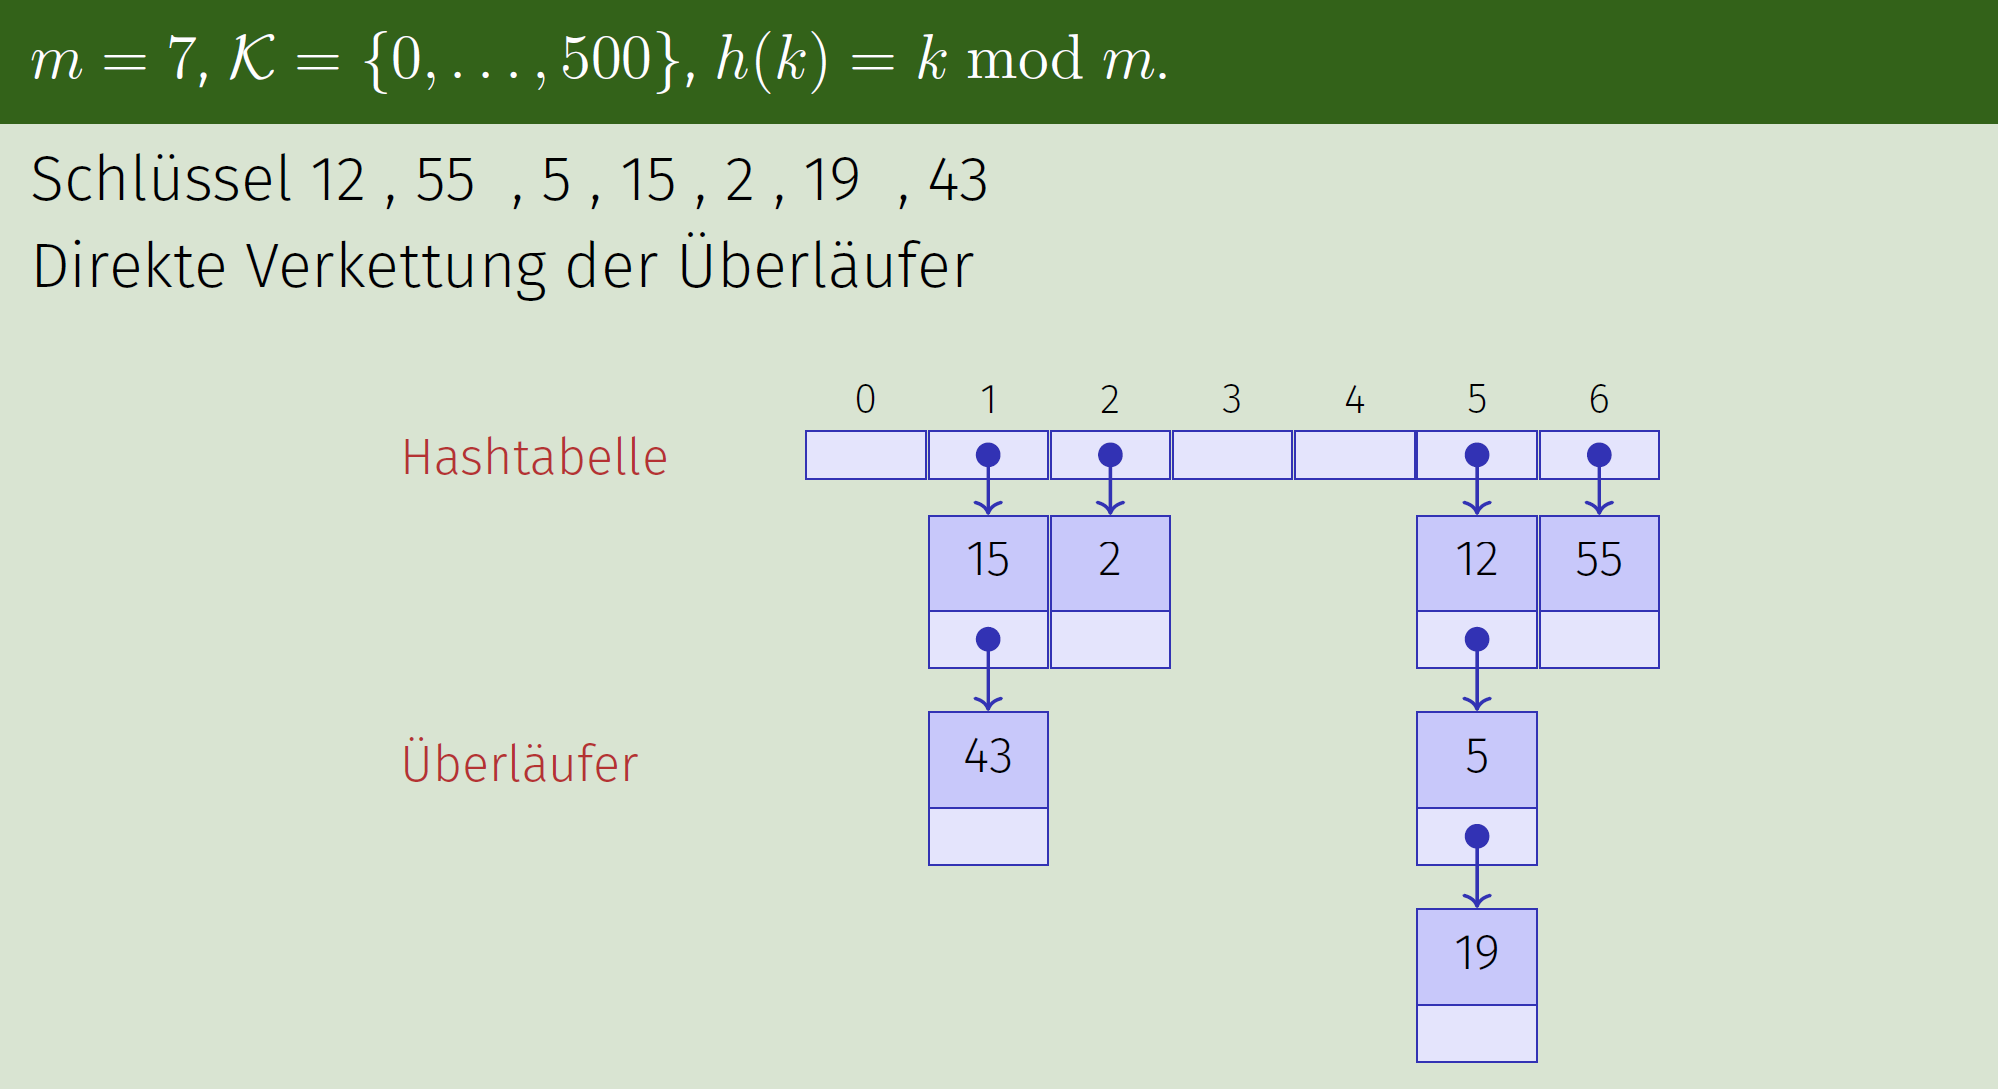
\includegraphics[width = \columnwidth]{../img/hashVerkettung.png}
\end{center}\smallskip

\textbf{Einfaches gleichmässiges Hashing}\par
Starke Annahmen: Jeder beliebige Schlüssel wird mit gleicher Wahrscheinlichkeit (\textbf{Uniformität}) und unabhängig von den anderen Schlüsseln (\textbf{Unabhängigkeit}) auf einen der $m$ verfügbaren Slots abgebildet.\par\smallskip
Unter dieser Annahme ergibt sich die \textbf{erwartete Länge}:\par $\mathbb{E}(\text { Länge Kette } j)=\frac{n}{m}=\alpha$, $\alpha$ heisst der \textbf{Belegungsfaktor} oder \textbf{Füllgrad}.\par\smallskip
Daraus ergibt sich (bei einfachem gleichmässigem Hashing) eine \textbf{erwartete Laufzeit (amortisiert)} von $\mathcal{O}(1)$ für Suchen, Einfügen, Löschen.\par\smallskip
\textbf{Vor- und Nachteile der Verkettung}\par
\begin{itemize}
    \item Belegungsfaktoren $\alpha > 1$ möglich; Entfernen von Schlüsseln einfach
    \item Speicherverbrauch der Verkettung
\end{itemize}\smallskip

\end{sectionbox}
\vspace{-4pt}
\begin{sectionbox}
\subsection{Konzept 2: Hashing mit offener Addressierung}\par\smallskip
\begin{itemize}
    \item Speichere die Überläufer direkt in der Hashtabelle mit einer \textbf{Sondierungsfunktion $s(k,j)$}
    \item Tabellenposition des Schlüssels entlang der \textbf{Sondierungsfolge $S(k)$}
\end{itemize}\par\smallskip
Technisches Detail zu \textbf{delete(k)}: Suche $k$ in der Tabelle gemäss $S(k)$. Ersetze $k$ durch den \textbf{speziellen Schlüssel removed}.\par\vspace{7px}
\end{sectionbox}
\vspace{-4pt}
\begin{sectionbox}
\subsubsection{Lineares Sondieren}\par\smallskip
\begin{center}
    $s(k, j)=h(k)+j \Rightarrow$ \par $S(k)=(h(k), h(k)+1, \ldots, h(k)+m-1) \bmod m$
\end{center}\par\smallskip
\textbf{Problem $\rightarrow$ Primäre Häufung}:\par Ähnliche Hashaddressen haben ähnliche Sondierungsfolgen $\rightarrow$ lange zusammenhängende belegte Bereiche.\par\smallskip
\textit{Beispiel}\par
\begin{center}
    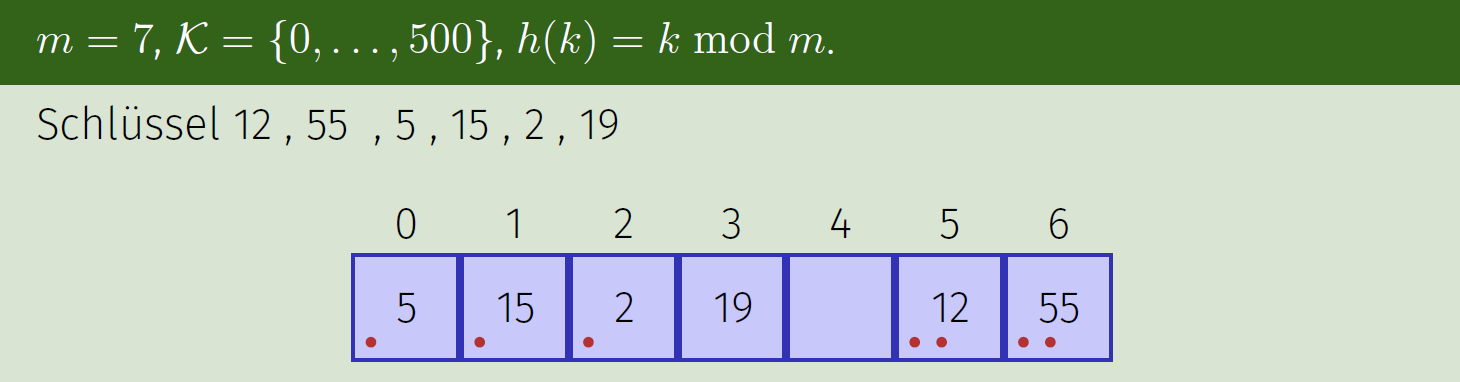
\includegraphics[width = 0.9\columnwidth]{../img/BspLinSond.png}
\end{center}
\end{sectionbox}
\vspace{-4pt}
\begin{sectionbox}
\subsubsection{Quadratisches Sondieren}\par\smallskip
\begin{center}
    $s(k, j)=h(k)+\lceil j / 2\rceil^{2}(-1)^{j+1}$
    $S(k)=(h(k), h(k)+1, h(k)-1, h(k)+4, h(k)-4, \ldots) \bmod m$
\end{center}\par\smallskip
\textbf{Problem $\rightarrow$ Sekundäre Häufung}:\par Synonyme $k$ und $k^{\prime}\left(\operatorname{mit} h(k)=h\left(k^{\prime}\right)\right)$ durchlaufen dieselbe Sondierungsfolge.\par\smallskip
\textit{Beispiel}\par
\begin{center}
    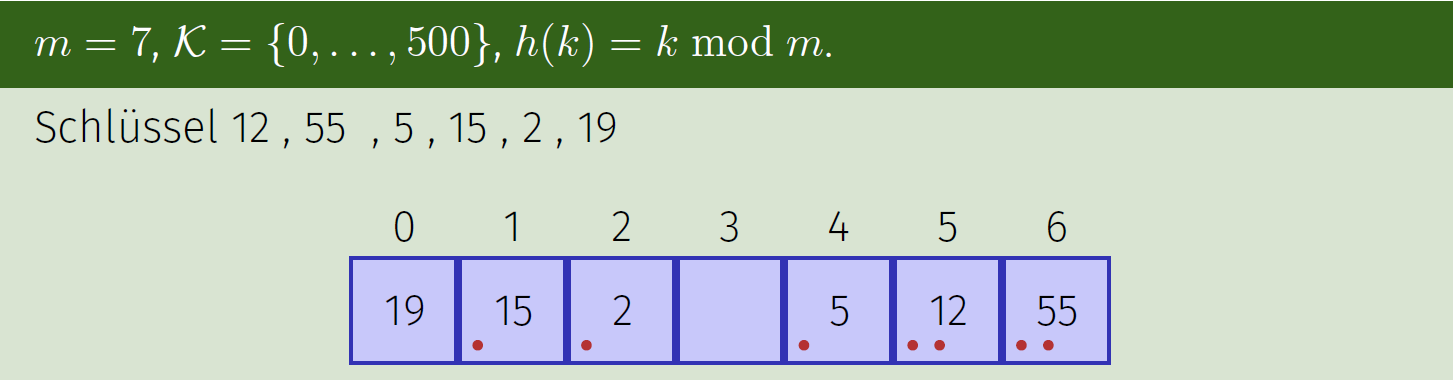
\includegraphics[width = 0.9\columnwidth]{../img/BspQuadSond.png}
\end{center}
\end{sectionbox}
\vspace{-4pt}
\begin{sectionbox}
\subsubsection{Double Hashing}\par\smallskip
Verwendung von zwei Hashfunktionen $h(k)$ und $h^{\prime}(k) \rightarrow$ Vermeidung primärer und sekundären Häufungen.
\begin{center}
    $s(k, j)=h(k)+j \cdot h^{\prime}(k)$\par
    $S(k)=(h(k), h(k)+h^{\prime}(k), h(k)+2 h^{\prime}(k)b, \ldots$ \par
    $, h(k)+(m-1) h^{\prime}(k)) \quad \bmod m$
\end{center}\par\smallskip

\textbf{Gleichmässiges Hashing}\par
Starke Annahme: Die Sondierungssequenz $S(k)$ eines Schlüssels $k$ ist mit gleicher Wahrscheinlichkeit eine der $m !$ vielen Permutationssequenzen von $\{0,1, \ldots, m-1\}$.
$\rightarrow$ Füllgrad $\alpha=$ $\frac{n}{m}<1$, so hat die nächste Operation erwartete Laufzeitkosten von $\leq \frac{1}{1-\alpha}$\par\smallskip
\textit{Beispiel}\par
\begin{center}
    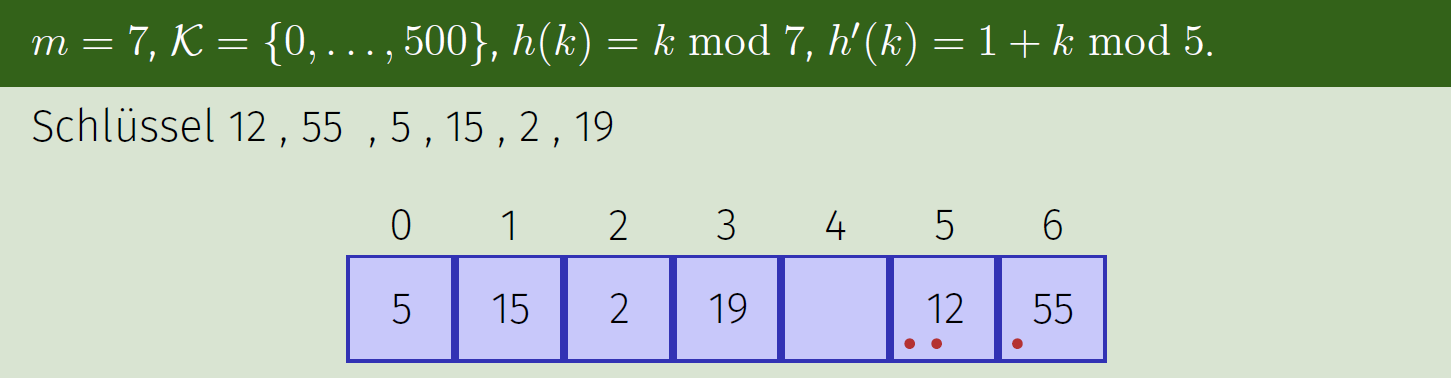
\includegraphics[width = 0.9\columnwidth]{../img/BespDoubHash.png}
\end{center}
\end{sectionbox}
\vspace{-4pt}
\begin{sectionbox}
\subsubsection{Beispiele}\par\smallskip
\begin{itemize}
    \item $h'(k) = \lceil \ln (k+1) \rceil \bmod q$: This function is not suitable as a second hash function, because for the key $k = 0$ we have $h'(0) = \lceil \ln (1) \rceil = 0$.
    \item $s(j,k) = k^j \bmod p$: This function is not suitable as a probing function, because for the keys $k = 0$ and $k = 1$, the function $s(j, k)$ has constant value of 0 and 1.
    \item $s(j,k) = ((k \cdot j) \bmod q) + 1$: This function is also not suitable as a probing function because its value is constant 1 if the key $k$ is a multiple of $q$.\par Moreover, for all other keys, the image of $s(j, k)$ is $\{1, . . . , q\}$, i.e., $p - q$ addresses of the hash table cannot be reached.
\end{itemize}

\end{sectionbox}

% SECTION ====================================================================================
\section{Graphen}
% ============================================================================================

\begin{sectionbox}
\subsection{Terminologie}\smallskip
Ein Graph $G=(V,E)$ besteht aus der Menge von Kanten $V=\{v_{1},\ldots,v_{1^n}\}$ und der Menge von Kanten $E$.\par\smallskip

\textbf{Gerichteter Graph}: $E \subseteq V \times V=\{(u, v): u \in V, v \in V\}$\par
\begin{itemize}
    \item $w \in V$ heisst \textbf{adjazent} zu $v \in V$, falls $(v, w) \in E$
    \item Vorgänger eines Knotens $v$: $N^{-}(v):=\{u \in V |(u, v) \in E\}$
    \item Nachfolger eines Knotens $v$: $N^{+}(v):=\{u \in V |(v, u) \in E\}$
    \item Eingangsgrad: $\operatorname{deg}^{-}(v):=|N^{-}(v)|$
    \item Ausngangsgrad: $\operatorname{deg}^{+}(v):=|N^{+}(v)|$
\end{itemize}\par\smallskip
\begin{center}
    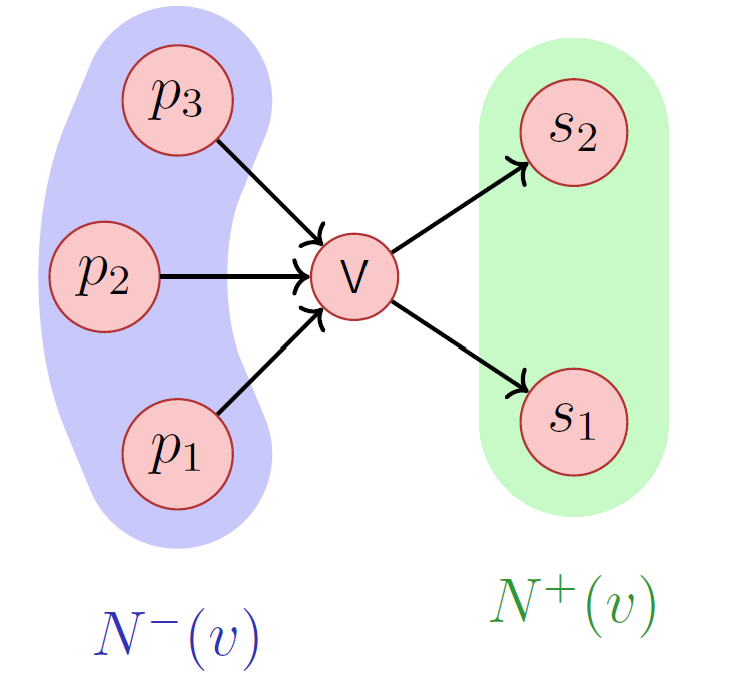
\includegraphics[width=0.5\columnwidth]{../img/gerGraph.png}
\end{center}\par\smallskip

\textbf{Unerichteter Graph}: $E \subseteq \{(u, v): v \in V, u \in V\}$\par
\begin{itemize}
    \item $w \in V$ heisst \textbf{adjazent} zu $v \in V$, falls $\{v, w\} \in E$
    \item Nachbarschaft: $N(v):=\{w \in V |\{v, w\} \in E\}$
    \item Grad: $\operatorname{deg}(v):=|N(v)|$ (Schleifen zählen 2)
\end{itemize}\par\smallskip

\textbf{Vollständiger Graph}: Ungerichteter Graph mit  $E=\{(u, v): u \in V, v \in V, \quad c \neq v\}$\par\smallskip
\textbf{Bipartiter Graph}: Graph, bei dem $V$ so in disjunkte $U$ und $W$ aufgeteilt werden kann, dass alle $e \in E$ einen Knoten in $U$ und einen in $W$ haben\par
%\begin{center}
%   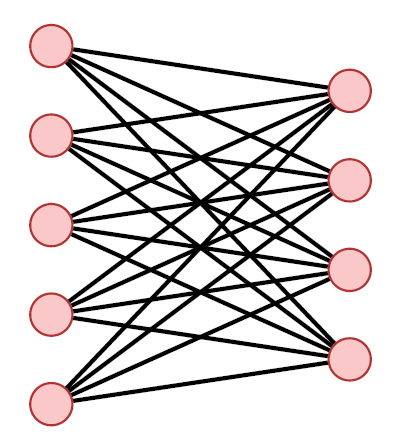
\includegraphics[width=0.25\columnwidth]{../img/biparGraph.png}
%\end{center}\par\smallskip
\textbf{Wege}:\par
\begin{itemize}
    \item \textbf{Weg / Path}: Sequenz von Knoten $p=\left\langle v_{1}, v_{2}, \ldots, v_{k}\right\rangle$ so dass für jedes $i \in\{1 \ldots k\}$ eine Kante von $v_{i}$ nach $v_{i+1}$ existiert
    \item \textbf{Pfad / einfacher Pfad / simple path}: Weg der keinen Knoten mehrfach verwendet
    \item \textbf{Länge des Weges}: Anzahl enthaltene Kanten $k$
    \item \textbf{Gewicht des Weges} (in gewichteten Graphen): $\sum_{i=1}^{k} c\left(\left(v_{i}, v_{i+1}\right)\right)$ (bzw. $\left.\sum_{i=1}^{k} c\left(\left\{v_{i}, v_{i+1}\right\}\right)\right)$
\end{itemize}\par\smallskip
\textbf{Zusammenhang}:\par
\begin{itemize}
    \item Ungerichteter Graph heisst \textbf{zusammenhängend}, wenn für jedes Paar $v, w \in V$ ein verbindender Weg existiert.
    \item Gerichteter Graph heisst \textbf{stark zusammenhängend}, wenn für jedes Paar $v, w \in V$ ein verbindender Weg existiert.
    \item Gerichteter Graph heisst \textbf{schwach zusammenhängend}, wenn der entsprechende ungerichtete Graph zusammenhängend ist.
\end{itemize}\par\smallskip
\textbf{Zyklen}:\par
\begin{itemize}
    \item \textbf{Zyklus}: Weg (und nicht einfacher Pfad!) $\left\langle v_{1}, \ldots, v_{k+1}\right\rangle$ mit $v_{1}=v_{k+1}$
    \item \textbf{Einfacher Zyklus}: Zyklus, aber Knoten kommen nicht mehrfach vor (ausser $s$ und $t$)
    \item \textbf{Kreis}: Zyklus mit paarweise verschiedenen $v_{1}, \ldots, v_{k},$ welcher keine Kante mehrfach verwendet
    \item \textbf{Kreisfrei (azyklisch)}: Graph ohne jegliche Kreise.
\end{itemize}\par\vspace{7px}

\subsubsection{Beobachtungen}\par
\begin{itemize}
    \item Allgemein: $0 \leq|E| \in \mathcal{O}\left(|V|^{2}\right)$
    \item Zusammenhängender Graph: $|E| \in \Omega(|V|)$
    \item Vollständiger Graph: $|E|=\frac{|V| \cdot(|V|-1)}{2}$ (ungerichtet)
    \item Maximal $|E|=|V|^{2}(\text { gerichtet })$
    \item Maximal $|E|=\frac{|V| \cdot(|V|+1)}{2}$ (ungerichtet)
\end{itemize}\par\smallskip
\end{sectionbox}

\vspace{100px}

\begin{sectionbox}
\subsection{Repräsentation von Graphen}\smallskip

\subsubsection{Adjazenzmatrix}\par\smallskip
Graph $G=(V, E)$ mit Knotenmenge $v_{1}, \ldots, v_{n}$ gespeichert als Adjazenzmatrix $A_{G}=\left(a_{i j}\right)_{1 \leq i, j \leq n}$ mit Einträgen aus $\{0,1\}$. $a_{i j}=1$ genau dann wenn Kante von $v_{i}$ nach $v_{j}$. Speicherbedarf $\Theta\left(|V|^{2}\right)$. $A_{G}$ ist symmetrisch, wenn $G$ ungerichtet.\par\smallskip
\begin{center}
    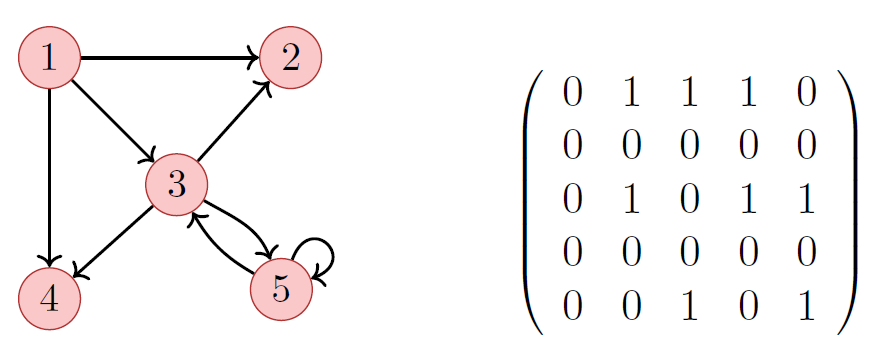
\includegraphics[width = 0.9\columnwidth]{../img/AdjMa.png}
\end{center}\vspace{10px}

\subsubsection{Adjazenzliste}\par\smallskip
Viele Graphen $G=(V, E)$ mit Knotenmenge $v_{1}, \ldots, v_{n}$ haben deutlich weniger als $n^{2}$ Kanten. Repräsentation mit Adjazenzliste: Array $A[1], \ldots, A[n]$, $A_{i}$ enthält verkettete Liste aller Knoten in $N^{+}\left(v_{i}\right)$. Speicherbedarf $\Theta\left(|V|+|E|\right)$.\par\smallskip
\begin{center}
    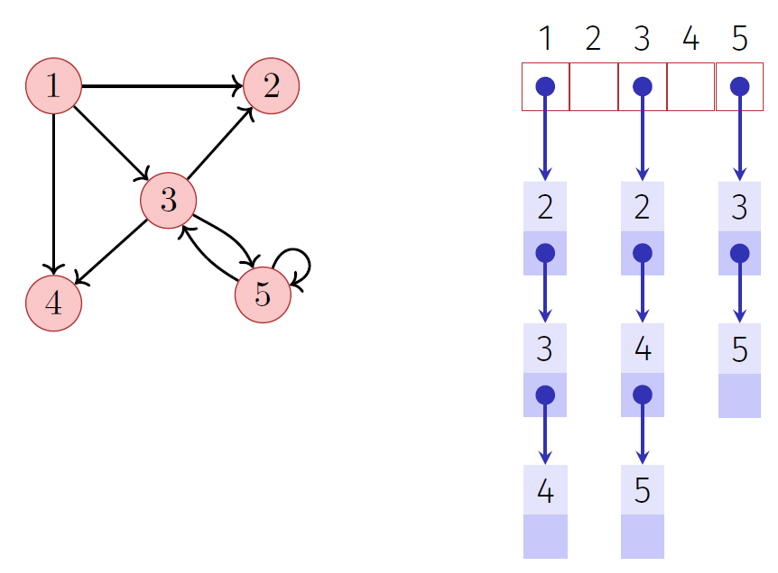
\includegraphics[width = 0.9\columnwidth]{../img/AdjList.png}
\end{center}\vspace{10px}

\subsubsection{Laufzeiten einfacher Operationen}\par\smallskip
\begin{center}
    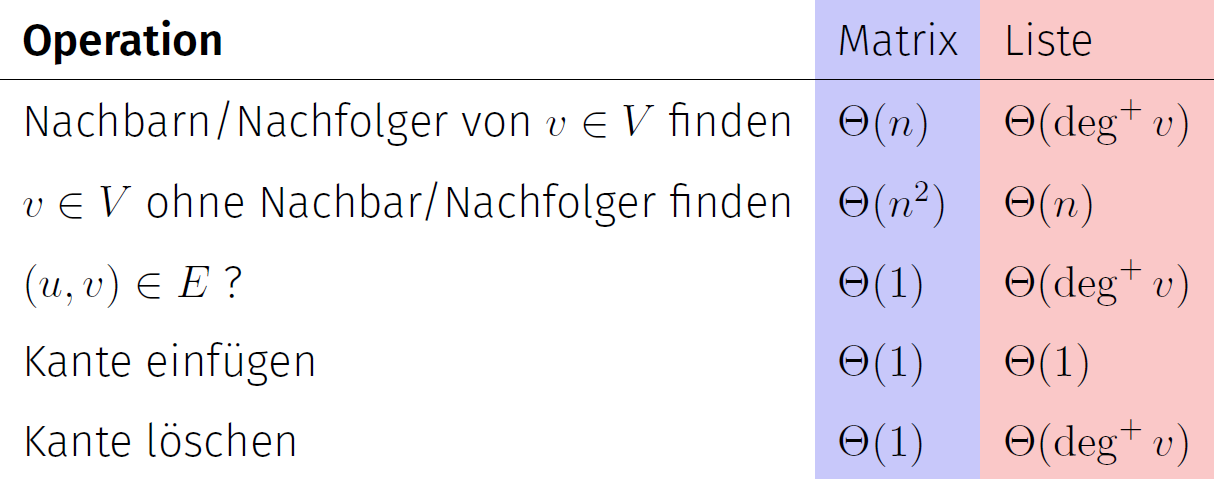
\includegraphics[width = \columnwidth]{../img/AdjLaufzeiten.png}
\end{center}\smallskip
\end{sectionbox}

\vspace{150px}

\begin{sectionbox}
\subsection{Graphen Traversieren: Tiefensuche}\smallskip
Verfolge zuerst Pfad in die Tiefe, bis nichts mehr besucht werden kann.\par
\begin{center}
    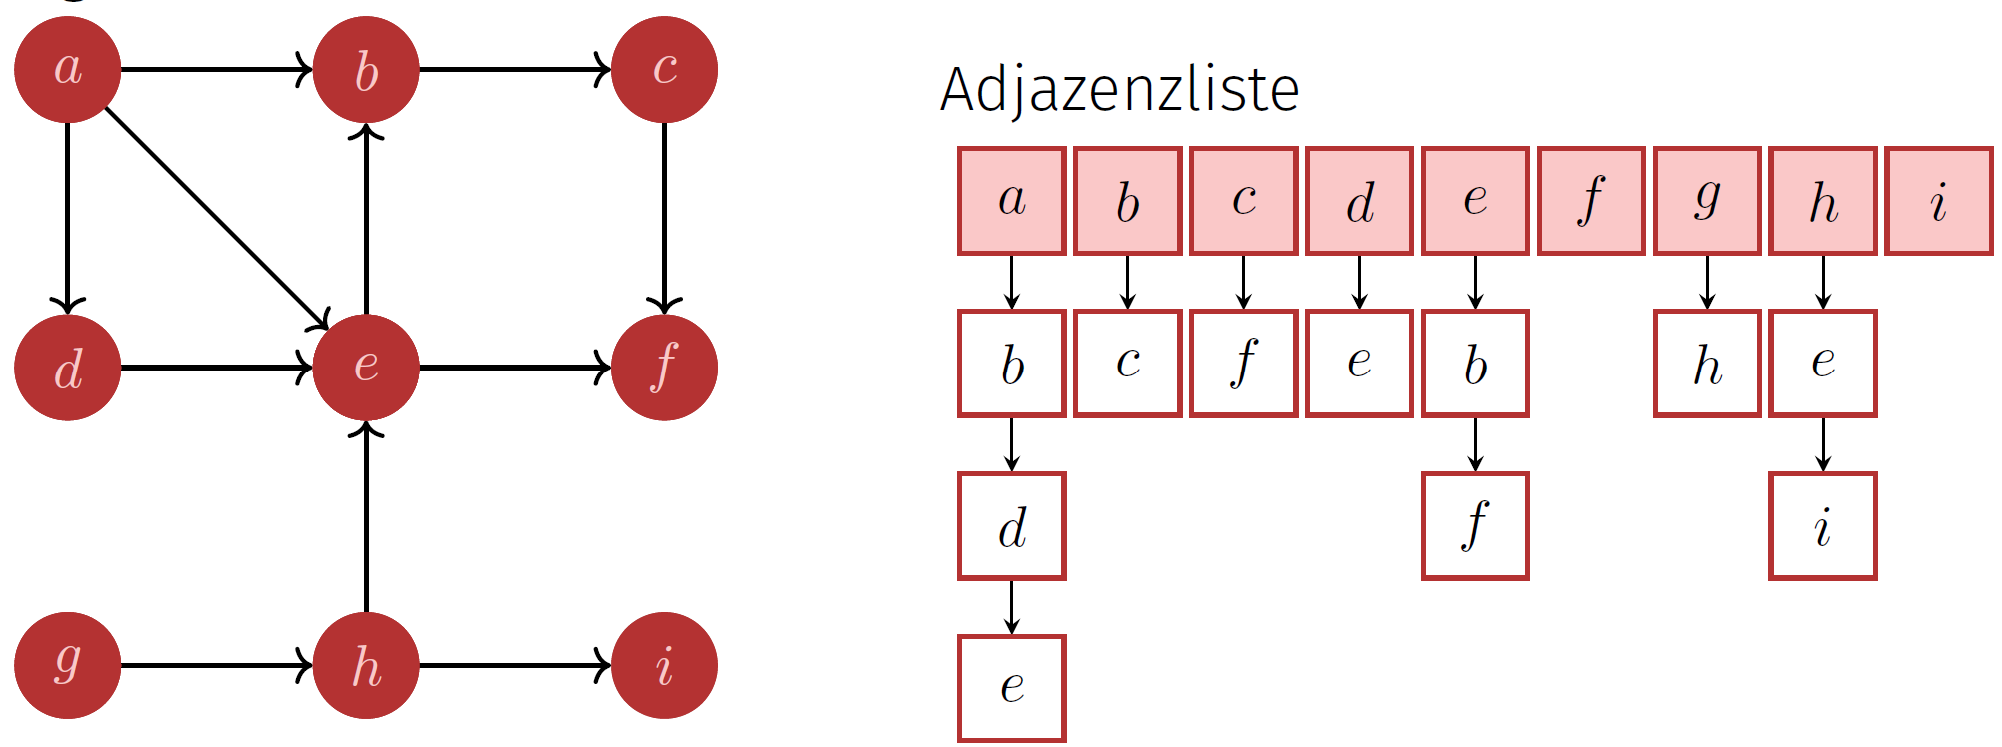
\includegraphics[width = 0.9\columnwidth]{../img/DFS_sym.png}
\end{center}\par
Reihenfolge: $a, b, c, f, d, e, g, h, i$\medskip

\textbf{Tiefensuche ab Knoten $v$: DFS-Visit(G,v)}\par
Laufzeit (ohne Rekursion): $\Theta\left(\operatorname{deg}^{+} v\right)$\par\smallskip

\textbf{Tiefensuche für alle Knoten: DFS-Visit(G)}\par
Laufzeit: $\Theta(|V|+\sum_{v \in V}(\operatorname{deg}^{+}(v)+1))=\Theta(|V|+|E|)$\par\smallskip

\begin{tabular*}{\columnwidth}{@{\extracolsep\fill}ll@{}}
\textbf{DFS-Visit(G,v)} & \textbf{DFS-Visit(G)} \\
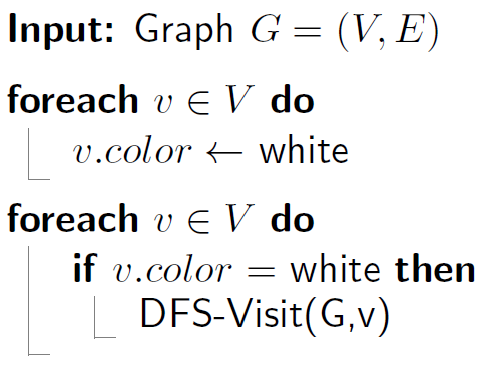
\includegraphics[width = 0.40\columnwidth]{../img/DFSG.png} &
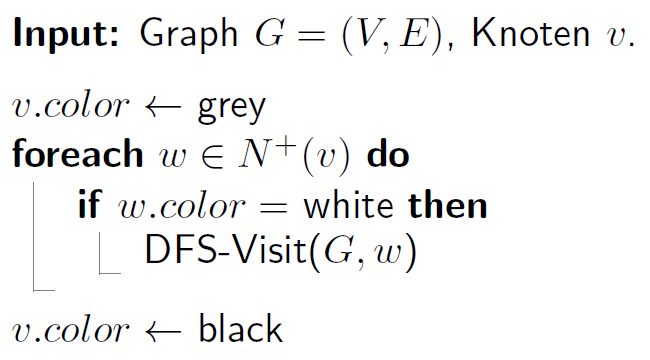
\includegraphics[width = 0.54\columnwidth]{../img/DFSGv.png} \\
\end{tabular*}\smallskip
\end{sectionbox}

\begin{sectionbox}
\subsection{Graphen Traversieren: Breitensuche}\smallskip
Verfolge zuerst Pfad in die Breite, gehe dann in die Tiefe.\par
\begin{center}
    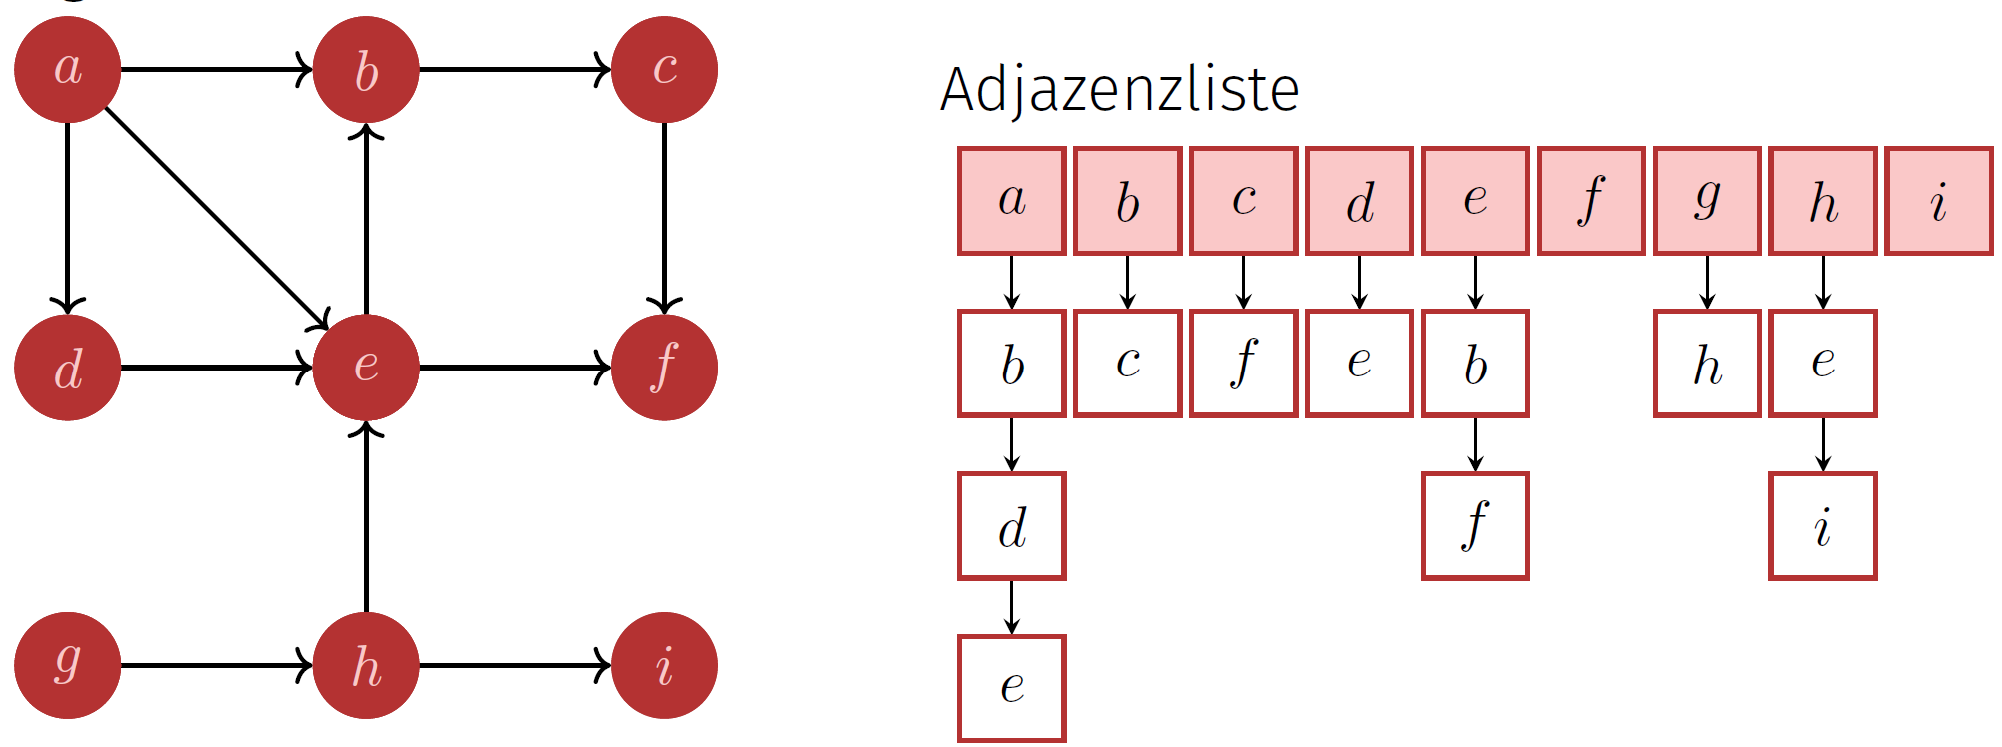
\includegraphics[width = 0.9\columnwidth]{../img/DFS_sym.png}
\end{center}\par
Reihenfolge: $a, b, d, e, c, f, g, h, i$\medskip

\begin{tabular*}{\columnwidth}{@{\extracolsep\fill}ll@{}}
\textbf{BFS-Visit(G,v)} & $\quad \quad \quad \quad$\textbf{BFS-Visit(G)} \\
\multicolumn{2}{l}{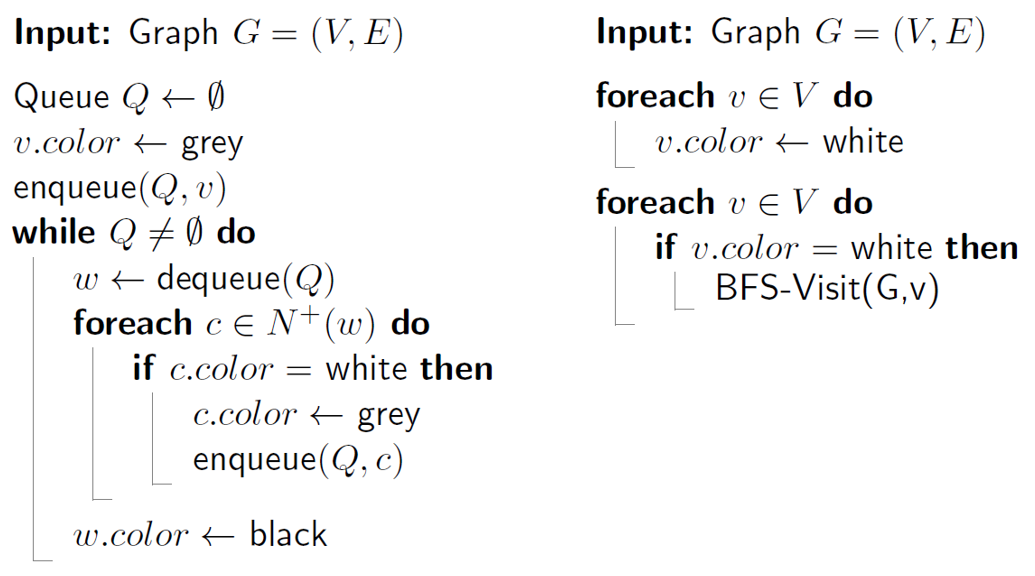
\includegraphics[width = 0.9\columnwidth]{../img/BFS.png}} \\
Extraplatz: $\mathcal{O}(|V|)$&  $\quad \quad \quad \quad$ Laufzeit: $\Theta(|V|+|E|)$ \\
\end{tabular*}

\end{sectionbox}

\begin{sectionbox}
\subsection{Topologische Sortierung}\smallskip
\begin{greenbox}
Ein gerichteter Graph $G=(V, E)$ besitzt genau dann eine topologische Sortierung, wenn er \textbf{kreisfrei} ist.
\end{greenbox}\smallskip

\begin{center}
    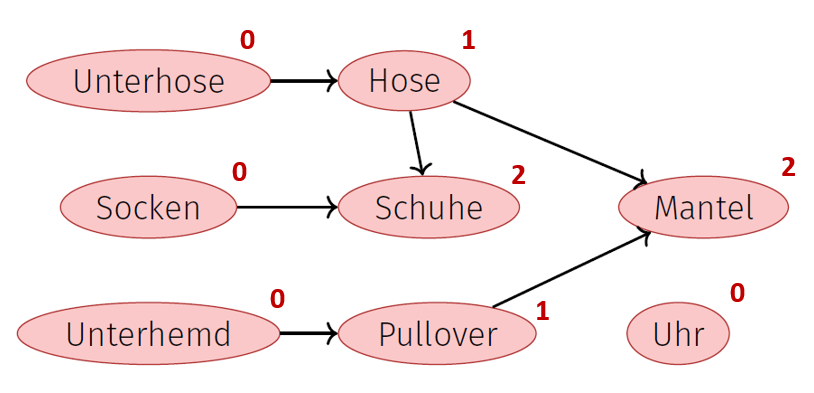
\includegraphics[width = 0.9\columnwidth]{../img/topoSort.png}
\end{center}\par\smallskip
Augmentiere den Eingangsgrad. Abbarbeitung nur wenn Eingangsgrad $0$ ist. Eingangsgrad verringern entspricht Knotenentfernen.\par\smallskip

\textbf{Topological-Sort(G)}\par
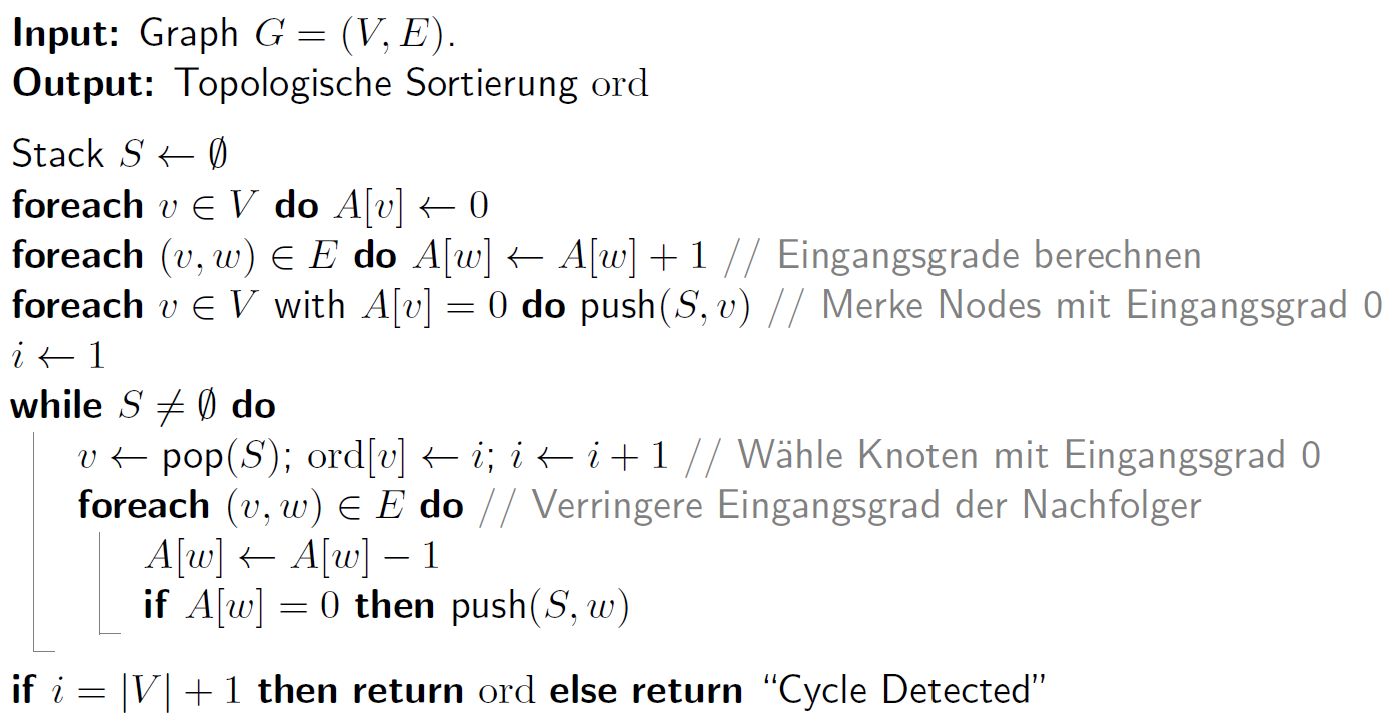
\includegraphics[width = \columnwidth]{../img/topoSortG.png}\par\smallskip

\textbf{Analyse}\par
\begin{itemize}
    \item Sei $G=(V, E)$ ein gerichteter, kreisfreier Graph. Der Algorithmus Topological-Sort berechnet in Zeit $\Theta(|V|+|E|)$ eine topologische Sortierung $\operatorname{ord}$ für $G$.
    \item Sei $G=(V, E)$ ein gerichteter, \textbf{nicht}-kreisfreier Graph. Der Algorithmus Topological-Sort terminiert in Zeit $\Theta(|V|+|E|)$ und detektiert den Zyklus.
\end{itemize}

\end{sectionbox}

\newpage

\begin{sectionbox}
\subsection{Kürzeste Wege}\smallskip
\textbf{Notation}\par\smallskip
$\delta(u, v)=$ Gewicht eines kürzesten Weges von $u$ nach $v$\par
$\delta(u, v)=\left\{\begin{array}{ll}
\infty & \text { kein Weg von } u \text { nach } v \\
\min \{c(p): u \stackrel{p}{\longrightarrow} v\} & \text { sonst }
\end{array}\right.$\par\smallskip

\textbf{Beobachtungen}\par
\begin{itemize}
    \item Einfachster Fall: Kantengewicht 1 $\rightarrow$ Breitensuche
    \item Es gibt Situationen, in denen kein kürzester Weg existiert: negative Zyklen könnten auftreten.
    \item Es kann exponentiell viele Wege geben $\rightarrow$  alle Wege probieren ist ineffizient
    \item Ein kürzester Weg von $s$ nach $v$ (ohne weitere Einschränkungen) kann nicht länger sein als ein kürzester Weg von $s$ nach $v$, der $u$ enthalten muss.\par
    \textcolor{tanne}{\textbf{$\delta(s, v) \leq \delta(s, u)+\delta(u, v)$}}
    \item \textbf{Optimale Substruktur}: Teilpfade von kürzesten Pfaden sind kürzeste Pfade ( \textbf{\textcolor{tanne}{Kürzester Pfad $\Rightarrow$ kürzeste Subpfäde}} )
    \item Kürzeste Wege enthalten keine Zyklen
\end{itemize}\par\vspace{10px}

\subsubsection{Allgemeiner Algorithmus (Relaxier-Algorithmus)}\smallskip
Gesucht: Kürzeste Wege von einem Startknoten $s$ aus.
\begin{itemize}
    \item Gewicht des kürzesten bisher gefundenen Pfades
    \begin{itemize}
        \item Zu Beginn: $d_{s}[v]=\infty$ für alle Knoten $v \in V$
        \item Ziel: $d_{s}[v]=\delta(s, v)$ für alle $v \in V$
    \end{itemize}
    \item Vorgänger eines Knotens: u Beginn $\pi_{s}[v]$ undefiniert für jeden Knoten $v \in V$
\end{itemize}\smallskip


\textbf{Algorithmus}\smallskip
\begin{enumerate}
    \item Initialisiere $d_{s}$ und $\pi_{s}: d_{s}[v]=\infty$, $\pi_{s}[v]=$ null für alle $v \in V$
    \item Setze $d_{s}[s] \leftarrow 0$
    \item Wähle eine Kante $(u, v) \in E$:\par
    \begin{greenbox}
    \textbf{Relaxiere $(u, v)$:}\par
    $\begin{array}{l}
    \text { if } d_{s}[v]>d[u]+c(u, v) \text { then } \\
    \qquad \begin{array}{l}
    d_{s}[v] \leftarrow d_{s}[u]+c(u, v) \\
    \pi_{s}[v] \leftarrow u
    \end{array}
    \end{array}$
    \end{greenbox}
    \item Wiederhole 3 bis nichts mehr relaxiert werden kann (bis $\left(d_{s}[v] \leq d_{s}[u]+c(u, v) \quad \forall(u, v) \in E\right)$)
\end{enumerate}\vspace{10px}

\subsubsection{Dijkstra Algorithmus}\smallskip
\textbf{Beobachtung}\par
\begin{center}
    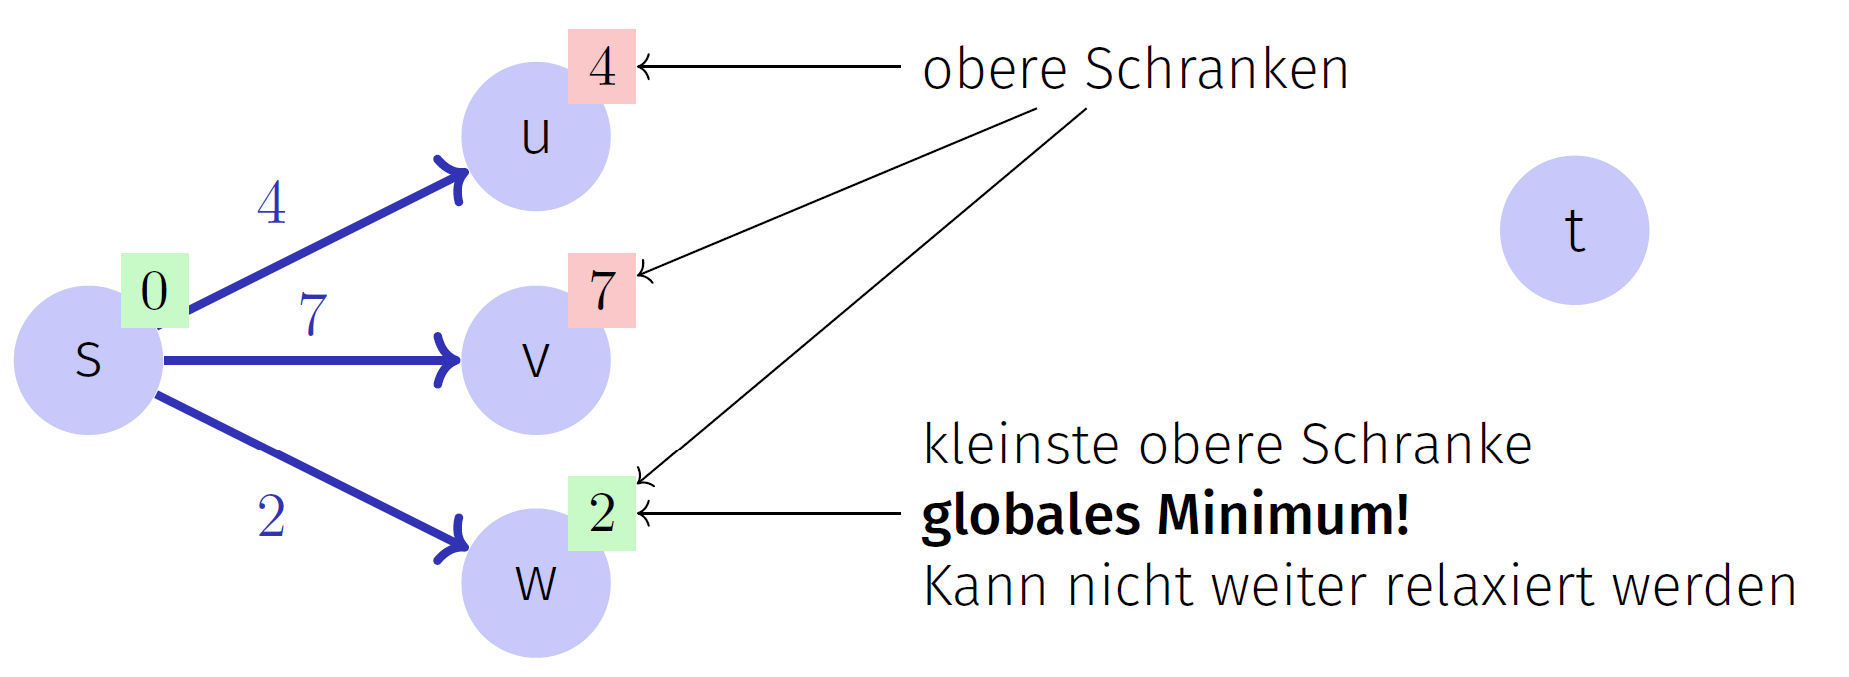
\includegraphics[width = 0.85\columnwidth]{../img/DijkstraBeobachtung.png}\par
\end{center}\smallskip

\textbf{Grundidee}\par
Menge $V$ aller Knoten wird unterteilt in
\begin{itemize}
    \item die \textcolor{red}{Menge $M$} von Knoten, für die schon ein kürzester Weg von $s$ bekannt ist
    \item die \textcolor{blue}{Menge $R=\cup_{v \in M} N^{+}(v) \backslash M$} von Knoten, für die kein kürzester Weg bekannt ist, die jedoch von $M$ direkt erreichbar sind.
    \item die \textcolor{orange}{Menge $U=V \backslash(M \cup R)$} von Knoten die noch nicht berücksichtigt wurden.
\end{itemize}

\begin{center}
    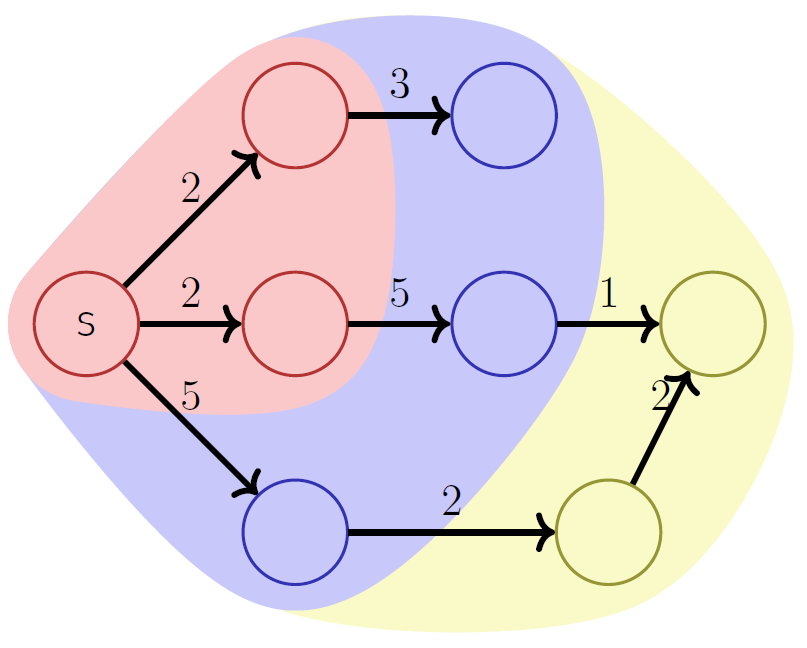
\includegraphics[width = 0.35\columnwidth]{../img/DijkstraSym.png}\par
\end{center}
\textit{Betrachte alle Nachbarn der Menge $M$ und füge den Knoten mit dem kürzesten Weg zu $s$ der Menge $M$ hinzu.}\par
\end{sectionbox}

\begin{sectionbox}
\textbf{Dijkstra(G,s)}\par
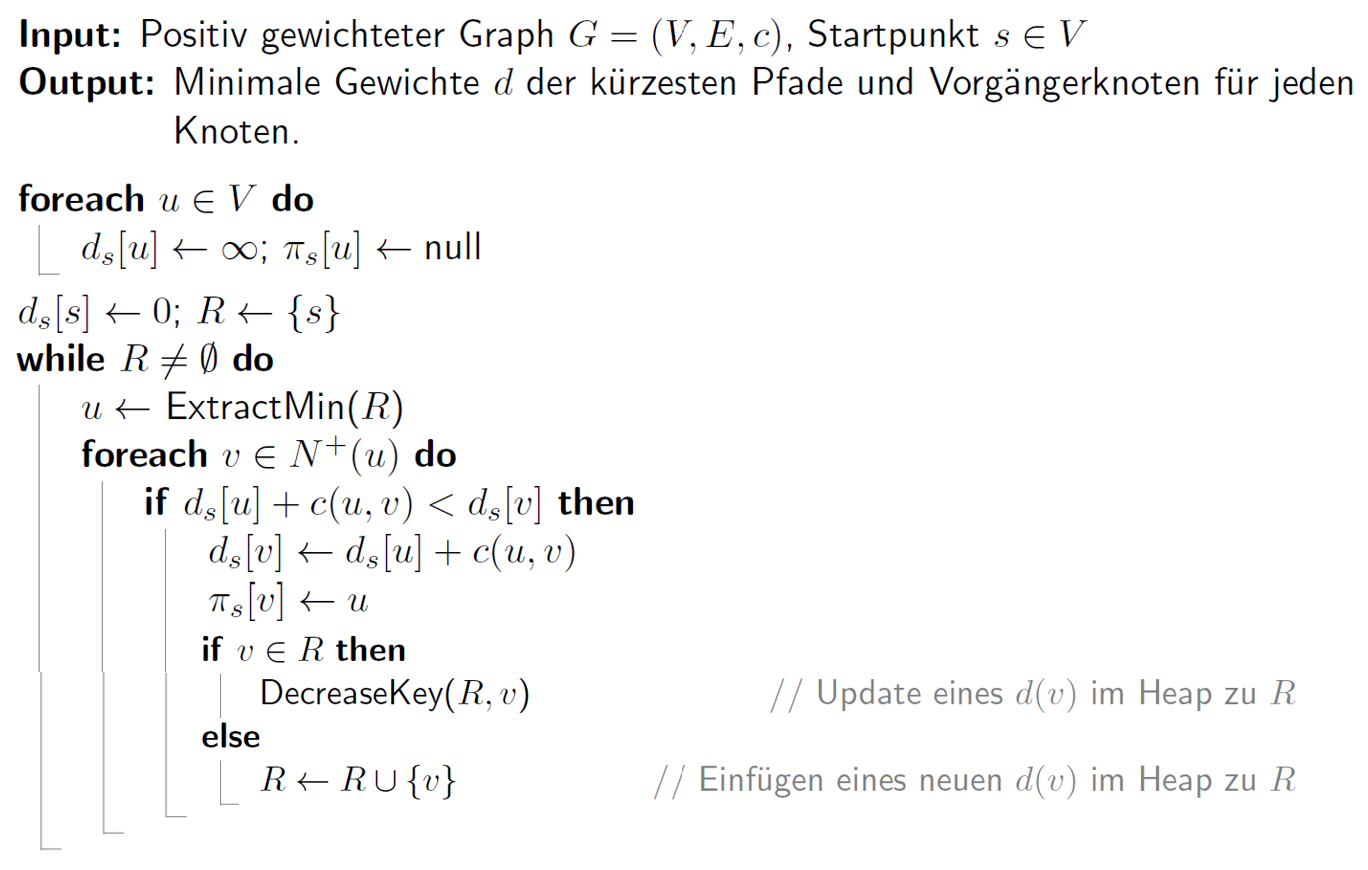
\includegraphics[width = \columnwidth]{../img/Dijkstra.png}\par
DecreaseKey (Aufsteigen im MinHeap), Position im Heap: Speichern am Knoten, Hashtabelle oder Lazy Deletion\par\smallskip
\textbf{Laufzeit}\par
\begin{itemize}
    \item $|V| \times$ ExtractMin: $\mathcal{O}(|V| \log |V|)$
    \item $|E| \times$ Insert oder DecreaseKey: $\mathcal{O}(|E| \log |V|)$
    \item $1 \times$ Init: $\mathcal{O}(|V|)$
    \item \textbf{Insgesamt}: $\mathcal{O}(|E| \log |V|)$
\end{itemize}

\end{sectionbox}
\begin{sectionbox}
\textit{Beispiel Dijkstra}\par
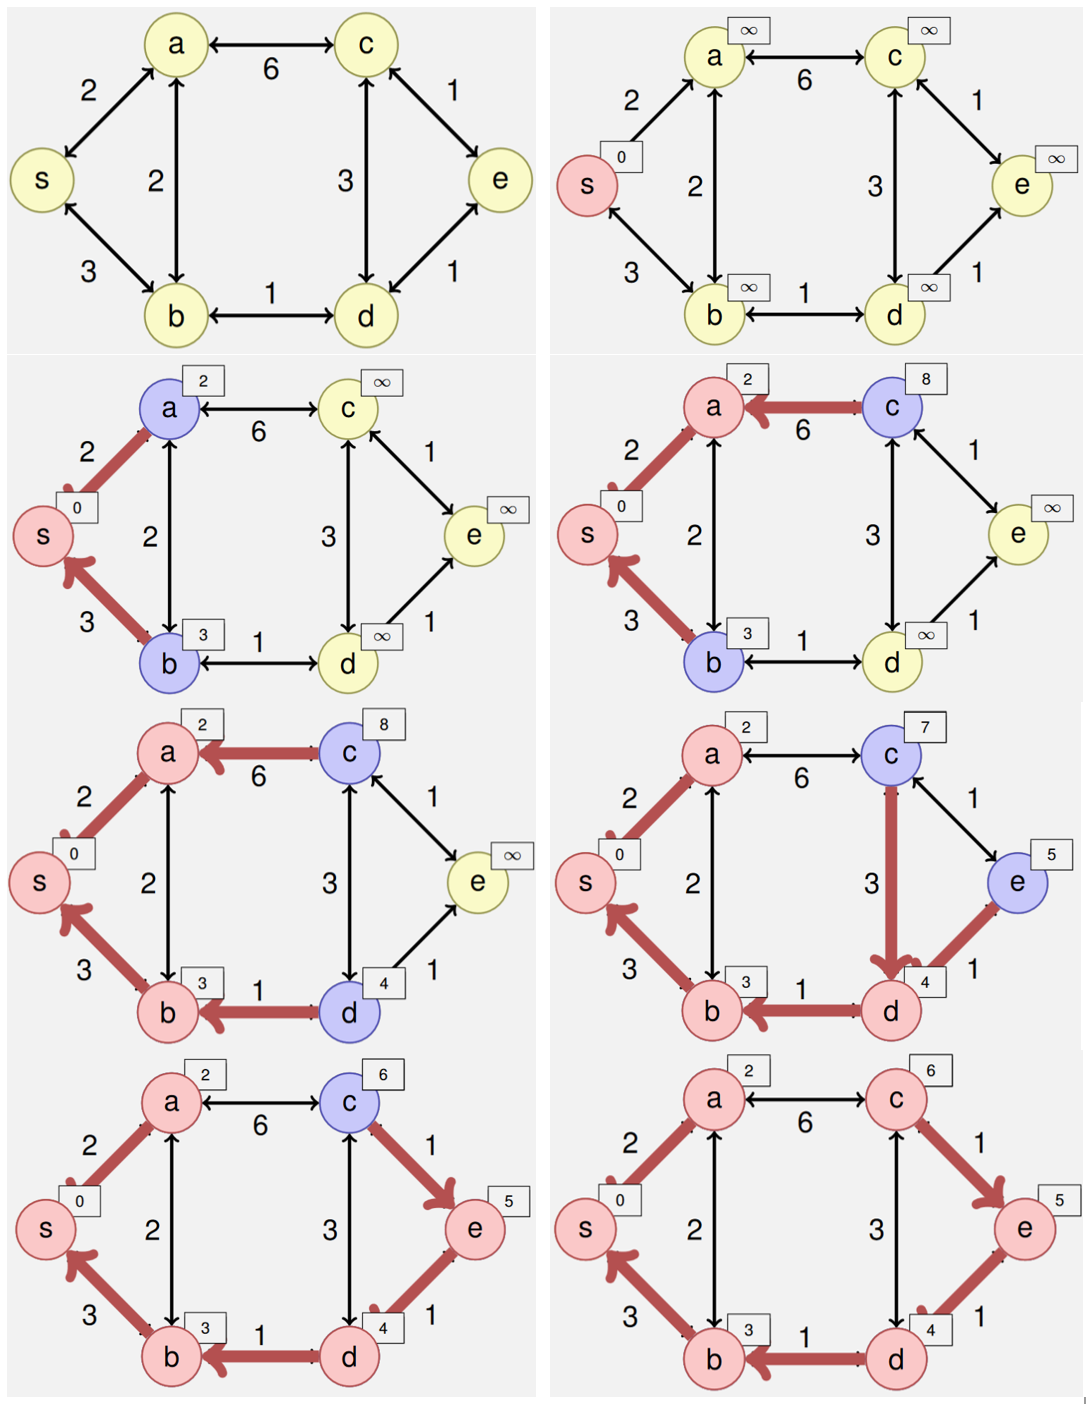
\includegraphics[width = \columnwidth]{../img/DijkstraBsp.png}\par
\end{sectionbox}

\vspace{300px}

\begin{sectionbox}
\subsection{Minimale Spannbäume}\smallskip
\textbf{Problem}\par
\begin{itemize}
    \item Gegeben: Ungerichteter, zusammenhängender, gewichteter Graph $G=(V, E, c)$
    \item Gesucht: Minimaler Spannbaum $T=\left(V, E^{\prime}\right)$ : zusammenhängender, zyklenfreier Teilgraph $E^{\prime} \subset E,$ so dass $\sum_{e \in E^{\prime}} c(e)$ minimal.
\end{itemize}
Greedy (gierige) Verfahren berechnen eine Lösung schrittweise, indem lokal beste Lösungen gewählt werden.\par\vspace{10px}

\subsubsection{Union-Find Kruskal Algorithmus}\smallskip
\textbf{Zur Implementation}\par
Gegeben eine Menge von Mengen $i \equiv A_{i} \subset V$. Zur Identifikation von Schnitten und Kreisen: Zugehörigkeit der beiden Endpunkte einer Kante zu einer der Mengen.\par
\begin{center}
    \includegraphics[width = 0.35\columnwidth]{../img/MST_Sym.png}\par
\end{center}\smallskip

Allgemeines Problem: Partition (Menge von Teilmengen) benötigt einen abstrakter Datentyp (\textbf{Union-Find}) mit folgenden Operationen:\par
\begin{itemize}
    \item Make-Set($(i)$): Hinzufügen einer neuen Menge $i$\par($p[i] \leftarrow i; return i$)
    \item Find ($e$): Name $i$ der Menge, welche $e$ enthält \par($\operatorname{while} (p[i]\neq 0) do\ i \leftarrow p[i]$; return $i$)
    \item Union($i,j$): Vereingung der Mengen mit Namen $i$ und $j$ \par($p[j]=i$, wobei $i$ und $j$ die Wurzeln (Namen) sind.)
\end{itemize}\smallskip
Laufzeitoptimierungen:\par
\begin{itemize}
    \item[a)] Immer kleineren Baum an grösseren hängen
    \item[b)] Bei Find Knoten immer an den Parent hängen
\end{itemize}\par\smallskip

\textit{Implementation von Union-Find}\par
Idee: Baum für jede Teilmenge in der Partition, z.B. {{1, 2, 3, 9}, {7, 6, 4}, {5, 8}, {10}}, wobei die Baumwurzeln $\to$ Namen (Stellvertreter) der Mengen ist.\par\smallskip
\begin{center}
    \includegraphics[width = 0.7\columnwidth]{../img/UF.png}\par\smallskip
    \includegraphics[width = 0.7\columnwidth]{../img/UFarray.png}\par\smallskip
\end{center}

\textbf{Algorithmus}\par
\includegraphics[width = \columnwidth]{../img/Kruskal.png}\par\smallskip

\textbf{Laufzeit des Kruskal Alghorithmus}\par
\begin{itemize}
    \item Sortieren der Kanten: $\Theta(|E| \log |E|)=\Theta(|E| \log |V|)$
    \item Initialisieren der Union-Find Datenstruktur $\Theta(|V|)$
    \item $|E| \times \text { Union }(\text { Find }(x), \text { Find }(y)): \mathcal{O}(|E| \log |V|)$
    \item \textbf{Insgesamt}: $\Theta(|E| \log |V|)$
\end{itemize}%\vspace{10px}
\end{sectionbox}

\begin{sectionbox}
\subsubsection{Algorithmus von Jarnik, Prim, Dijkstra}\smallskip
Idee: Starte mit einem $v \in V$ und lasse von dort unter Verwendung der Auswahlregel einen Spannbaum wachsen:\par
\includegraphics[width = 0.9\columnwidth]{../img/MST_JPD.png}\par\smallskip
\textit{Bemerkungen}\par
\begin{itemize}
    \item Man braucht keine Union-Find Datenstruktur (Färbung reicht aus)
    \item Vorgehensweise:
    \par \tab a) Immer Knoten mit kleinstem Gewicht zur Menge S hinzufügen
    \par \tab b) Wenn der Knoten noch nicht in S ist $\to$ MST ist zyklenfrei
\end{itemize}\par\smallskip
\textbf{Laufzeit insgesamt}: $\mathcal{O}(|E| \log |V|)$
\end{sectionbox}

% % SECTION ====================================================================================
\vspace{-4pt}
\begin{sectionbox}
\section{Flüsse in Netzen}
% ============================================================================================
\subsection{Terminologie und Eigenschaften}\medskip
\textbf{Flussnetzwerk}\par
\begin{itemize}
    \item Flussnetzwerk $G=(V, E, c):$ gerichteter Graph mit Kapazitäten
    \item Antiparallele Kanten verboten
    \item Quelle $s$ und Senke $t:$ spezielle Knoten. Jeder Knoten $v$ liegt auf einem Pfad zwischen $s$ und $t: s \leadsto v \leadsto t$
\end{itemize}\par\smallskip
\begin{center}
    \includegraphics[width = 0.9\columnwidth]{../img/flussNet.png}
\end{center}

\textbf{Fluss}  $f: V \times V \rightarrow \mathbb{R}$ erfüllt Bedingungen:\par
\begin{itemize}
    \item \textbf{Kapazitätsbeschränkung}: $\forall u, v \in V: f(u, v) \leq c(u, v)$
    \item \textbf{Schiefsymmetrie}: $\forall u, v \in V: f(u, v)=-f(v, u)$
    \item \textbf{Flusserhaltung}: $u \in V \backslash\{s, t\}: \sum_{v \in V} f(u, v)=0$
    \item \textbf{Wert $w$ des Flusses}:$|f|=\sum_{v \in V} f(s, v)$
\end{itemize}\par\smallskip
\end{sectionbox}
\vspace{-4pt}
\begin{sectionbox}
\begin{cookbox}{Eigenschaften}
\item $|f|=f(s, V)$
\item $f(U, U)=0$
\item $f\left(U, U^{\prime}\right)=-f\left(U^{\prime}, U\right)$
\item $f(X \cup Y, Z)=f(X, Z)+f(Y, Z),$ wenn $X \cap Y=\emptyset$
\item $f(R, V)=0 \text { wenn } R \cap\{s, t\}=\emptyset . \text { [Flusserhaltung! }]$\smallskip
\par Wobei gilt:
\par $f\left(U, U^{\prime}\right):=\sum\limits_{u \in U \atop u^{\prime} \in U^{\prime}} f\left(u, u^{\prime}\right)$, $f\left(u, U^{\prime}\right):=f\left(\{u\}U^{\prime}\right)$
\end{cookbox}\medskip
\end{sectionbox}
\vspace{-4pt}
\begin{sectionbox}
\textbf{Restnetzwerk}\par
Restnetzwerk $G_{f}$ gegeben durch alle Kanten mit Restkapazität. Restnetzwerke haben dieselben Eigenschaften wie Flussnetzwerke, ausser dass antiparallele Kapazitäten-Kantenzugelassen sind.\par\smallskip
\begin{center}
    \includegraphics[width = 0.9\columnwidth]{../img/restNet.png}
\end{center}\par\smallskip

\textbf{Erweiterungspfade}\par
\begin{itemize}
    \item \textbf{Erweiterungspfad $p$}: einfacher Pfad von $s$ nach $t$ im Restnetzwerk $G_{f}$
    \item \textbf{Restkapazität} $c_{f}(p)=\min \left\{c_{f}(u, v):(u, v) \text { Kante in } p\right\}$
\end{itemize}

\end{sectionbox}
\vspace{-4pt}
\begin{sectionbox}
\subsection{Maximaler Fluss / Minimaler Schnitt}\smallskip
\begin{emphbox}
$|f| \leq \sum\limits_{v \in S, v^{\prime} \in T} c\left(v, v^{\prime}\right)=c(S, T)$
\end{emphbox}
Wobei $S$ die Menge der Knoten vor dem Cut und $T$ die Menge der Knoten nach dem Cut ist. Gezählt werden folglich nur die Kapazitäten von $S$ zu $T$ und nicht alle! So ergibt dies im Beispiel: $c(S,T)=12+7+4=23$\par\smallskip

\begin{center}
    \includegraphics[width = 0.9\columnwidth]{../img/maxFlow.png}
\end{center}\par\smallskip

\begin{greenbox}
\textbf{Max-Flow Min-Cut Theorem}\par
Wenn $f$ ein Fluss in einem Flussnetzwerk $G=(V, E, c)$ mit Quelle $s$ und Senke $t$ ist, dann sind folgende Aussagen äquivalent:
\begin{enumerate}
    \item $f$ ist ein maximaler Fluss in $G$
    \item Das Restnetzwerk $G_{f}$ enthält keine Erweiterungspfade
    \item Es gilt $|f|=c(S, T)$ für einen Schnitt $(S, T)$ von $G$
\end{enumerate}
\end{greenbox}\vspace{10px}
\end{sectionbox}
\vspace{-4pt}
\begin{sectionbox}
\subsubsection{Die Ford-Fulkerson Methode}\smallskip
\begin{itemize}
    \item Starte mit $f(u, v)=0$ für alle $u, v \in V$
    \item Bestimme Restnetzwerk $G_{f}$ und Erweiterungspfad in $G_{f}$
    \item Erhöhe Fluss über den Erweiterungspfad
    \item Wiederholung bis kein Erweiterungspfad mehr vorhanden.
\end{itemize}\smallskip

\textbf{Ford-Fulkerson(G,s,t)}\par
\includegraphics[width = 0.8\columnwidth]{../img/FoFu.png}\par\smallskip

\textit{Praktische Anmerkung zur Implementierung}\par
In einer Implementation des Ford-Fulkerson Algorithmus müssen die negativen Flusskanten nicht unbedingt gespeichert werden, da ihr Wert sich stets als der negierter Wert der Gegenkante ergibt. Somit kann dies vereinfacht folgendermassen implementiert werden:\par\smallskip
\includegraphics[width = 0.45\columnwidth]{../img/paFF1.png} wird zu
\includegraphics[width = 0.4\columnwidth]{../img/paFF2.png}\par\smallskip

\textbf{Analyse}\par
Der Ford-Fulkerson Algorithmus muss für irrationale Kapazitäten nicht einmal terminieren! Sonst $\mathcal{O}\left(f_{\max }\cdot |E|\right)$.\vspace{10px}
\end{sectionbox}
\vspace{-4pt}
\begin{sectionbox}
\subsubsection{Edmonds-Karp Algorithmus}\smallskip
Wähle in der Ford-Fulkerson-Methode zum Finden eines Pfades in $G_{f}$ jeweils einen Erweiterungspfad kürzester Länge (z.B. durch Breitensuche).\par $\Rightarrow$ Gesamte asymptotische Laufzeit: $\mathcal{O}\left(|V| \cdot|E|^{2}\right)$

\end{sectionbox}
\vspace{-4pt}
\begin{sectionbox}
\subsection{Bipartites Matching}\smallskip
Konstruiere zur einer Partition $L, R$ eines bipartiten Graphen ein korrespondierendes Flussnetzwerk mit Quelle $s$ und Senke $t,$ mit gerichteten Kanten von $s$ nach $L$, von $L$ nach $R$ und von $R$ nach $t$. Jede Kante bekommt Kapazität 1.\par
\includegraphics[width = \columnwidth]{../img/biMa.png}\par\smallskip
\end{sectionbox}
\vspace{-4pt}
\begin{sectionbox}
\subsection{Anwendungen vom Maximalen Fluss}\medskip

\textbf{Knotenkapazitäten in Graphen einbauen}\par
\includegraphics[width = \columnwidth]{../img/KontenKap.png}\par
\textit{Trick}: Um Knotenkapazitäten in einen Graphen einzubauen muss man aus einem Knoten zwei machen (\textbf{Input-Knoten} und \textbf{Output-Knoten}). Die Kante zwischen dem Input-Knoten und dem Output-Knoten muss die Kapazität des Knotens haben. D.h. $c(v) = c(v,v')$\par\smallskip
\end{sectionbox}

% SECTION ====================================================================================
\vspace{-4pt}
\begin{sectionbox}
\section{Dynamische Programmierung}
% ============================================================================================
\subsection{Idee}\smallskip
\begin{itemize}
    \item Aufteilen eines komplexen Problems in eine vernünftige Anzahl kleinerer Teilprobleme
    \item Die Lösung der Teilprobleme wird zur Lösung des komplexeren Problems verwendet
    \item Identische Teilprobleme werden nur einmal gerechnet
\end{itemize}\smallskip
$\rightarrow$ Wir tauschen Laufzeit gegen Speicherplatz
\end{sectionbox}
\vspace{-4pt}
\begin{sectionbox}
\subsection{Dynamic Programming vs. Divide-And-Conquer}\smallskip
\begin{itemize}
    \item \textbf{Optimale Substruktur}: In beiden Fällen ist das Ursprungsproblem (einfacher) lösbar, indem Lösungen von Teilproblemen herangezogen werden können.
    \item Bei Divide-And-Conquer Algorithmen sind \textbf{Teilprobleme unabhängig}; deren Lösungen werden im Algorithmus nur einmal benötigt.\par
    Beim DP sind Teilprobleme nicht unabhängig. Das Problem hat \textbf{überlappende Teilprobleme}, welche im Algorithmus mehrfach gebraucht werden.
    \item Identische Teilprobleme werden nur einmal gerechnet d.h. \textbf{keine zirkulären Abhängigkeiten zwischen Teilproblemen}
\end{itemize}\smallskip
\end{sectionbox}
\vspace{-4pt}
\begin{sectionbox}
\subsection{Memoization}\smallskip
Memoization (sic) Abspeichern von Zwischenergebnissen.
\begin{itemize}
    \item Bevor ein Teilproblem gelöst wird, wird Existenz eines entsprechenden Zwischenergebnis geprüft
    \item Existiert ein gespeichertes Zwischenergebnis bereits, so wird dieses verwendet.
    \item Andernfalls wird der Algorithmus ausgeführt und das Ergebnis wird entsprechend gespeichert
\end{itemize}\smallskip
\end{sectionbox}
\vspace{-4pt}
\begin{sectionbox}
\textit{Beispiel Fibonacci}\par
\begin{center}
    \includegraphics[width = \columnwidth]{../img/memo.png}\par\smallskip
    \includegraphics[width = 0.54\columnwidth]{../img/Memo_Fib_schema_vor.png}
    \includegraphics[width = 0.45\columnwidth]{../img/Memo_Fib_schema.png}
\end{center}
$\rightarrow$ Genau hingesehen lösen wir das Problem bottom-up

\end{sectionbox}
\vspace{-4pt}
\begin{sectionbox}
\subsection{Dynamic Programming: Beschreibung am Beispiel}\smallskip

\textit{Beispiel Fibonacci}\par
\begin{center}
    \includegraphics[width = \columnwidth]{../img/DPtable.png}
\end{center}\smallskip

\end{sectionbox}
\vspace{-4pt}
\begin{sectionbox}
\subsection{Wie findet man den DP Algorithmus?}\smallskip
\begin{enumerate}
    \item Genaue Formulierung der gesuchten Lösung
    \item Definiere Teilprobleme (und bestimme deren Anzahl)
    \item Raten / Aufzählen (und bestimme die Laufzeit für das Raten)
    \item Rekursion: verbinde die Teilprobleme
    \item Memoisieren / Tabellieren. Bestimme die Abhängigkeiten der Teilprobleme
    \item Lösung des Problems: \par Laufzeit = Anz. Teilprobleme $\times$ $\frac{\text{Zeit}}{\text{Teilproblem}}$
\end{enumerate}

\end{sectionbox}
\vspace{-4pt}
\begin{sectionbox}
\subsection{Beispiel Kaninchen}\smallskip
Ein Kaninchen sitzt auf Platz (1,1) eines $n \times n$ Gitters. Es kann nur nach Osten oder nach Süden gehen. Auf jedem Wegstück liegt eine Anzahl Rüben. Wie viele Rüben sammelt das Kaninchen maximal ein?\par\smallskip
\begin{center}
    \includegraphics[width = 0.65\columnwidth]{../img/kan1.png}
\end{center}
\end{sectionbox}
\vspace{-4pt}
\begin{sectionbox}
\textbf{Rekursion}\par
Gesucht: $T_{0,0}=$ Maximale Anzahl Rüben von (0,0) nach $(n, n)$ Sei $w_{(i, j)-\left(i^{\prime}, j^{\prime}\right)}$ Anzahl Rüben auf Kante von $(i, j)$ nach $\left(i^{\prime}, j^{\prime}\right)$ Rekursion (maximale Anzahl Rüben von $(i, j) \text { nach }(n, n))$\par\smallskip
\begin{center}
    \includegraphics[width = \columnwidth]{../img/kanRek.png}
\end{center}
\textbf{Teilabhängigkeitsgraph}\par
\begin{itemize}
    \item Richtung der Abhängigkeiten: Links oben nach rechts unten
    \item Richtung der Berechung: Rechts unten nach links oben
\end{itemize}

\end{sectionbox}
\vspace{-4pt}
\begin{sectionbox}
\textbf{Bottom-Up Beschreibung am Beispiel}\par
\begin{center}
    \includegraphics[width = \columnwidth]{../img/kanTable.png}
\end{center}\smallskip

\end{sectionbox}

\vspace{-4pt}
\begin{sectionbox}
\subsection{Die Editierdistanz / Levenshteinabstand}\smallskip
\textbf{Aufgabenstellung}\par
\begin{center}
    \includegraphics[width = \columnwidth]{../img/ed1.png}
\end{center}
\end{sectionbox}
\vspace{-4pt}
\begin{sectionbox}
\textbf{Wie findet man den DP Algorithmus?}\par
\begin{enumerate}
    \item Genaue Formulierung der gesuchten Lösung:
    \par $E(n, m)=$ minimale Anzahl Editieroperationen (ED Kosten) für $a_{1 \ldots n} \rightarrow b_{1 \ldots m}$
    \item Definiere Teilprobleme (und bestimme deren Anzahl):
    \par Teilprobleme $E(i, j)=$ ED von $a_{1 \dots i} . b_{1 \dots j}$ (Anz. $n \cdot m$)
    \item Raten / Aufzählen (und bestimme die Laufzeit für das Raten):
    \par $a_{1 . . i} \rightarrow a_{1 \ldots i-1}(\text { löschen })$
    $a_{1 . . i} \rightarrow a_{1 \ldots i} b_{j}$ (einfügen)
    $a_{1 . . i} \rightarrow a_{1 \ldots i-1} b_{j}$ (ersetzen)
    \item Rekursion: verbinde die Teilprobleme:
    \par \begin{center}
        $E(i, j)=\min \left\{\begin{array}{l}\operatorname{del}\left(a_{i}\right)+E(i-1, j) \\ \operatorname{ins}\left(b_{j}\right)+E(i, j-1) \\ \operatorname{repl}\left(a_{i}, b_{j}\right)+E(i-1, j-1)\end{array}\right.$
    \end{center}
    \item Memoisieren / Tabellieren. Bestimme die Abhängigkeiten der Teilprobleme:
    \par \begin{center}
        \includegraphics[width=0.3\columnwidth]{../img/Lst_Abh.png}
    \end{center}
    \par Berechnung von links oben nach rechts unten. Zeilen- oder Spaltenweise.
    \item Lösung des Problems: Lösung steht in $E(n, m)$
\end{enumerate}
\end{sectionbox}
\vspace{-4pt}
\begin{sectionbox}
\textbf{Bottom-Up Beschreibung}\par
\begin{center}
    \includegraphics[width = \columnwidth]{../img/edTable.png}
\end{center}\smallskip

\textbf{Analyse}\par
Anzahl Tabelleneinträge: $(m+1) \cdot (n+1)$\par
Laufzeit: $\mathcal{O}(m \cdot n)$\smallskip
\end{sectionbox}
\vspace{-4pt}
\begin{sectionbox}
\subsection{Kürzeste Wege: DP Ansatz (Bellman)}\smallskip
Induktion über Anzahl Kanten $d_{s}[i, v]$: Kürzeste Weglänge von $s$ nach $v$ über maximal $i$ Kanten.\par\vspace{-3px}
\begin{equation*}
\begin{array}{l}
d_{s}[i, v]=\min \left\{\begin{array}{l} d_{s}[i-1, v] \\ \min _{(u, v) \in E}\left(d_{s}[i-1, u]+c(u, v)\right)\end{array}\right. \\
d_{s}[0, s]=0, \underbrace{d_{s}[0, v]=\infty \forall v \neq s}_{\text{Zyklus}}
\end{array}
\end{equation*}\par\smallskip
\begin{center}
    \includegraphics[width = 0.9\columnwidth]{../img/BellFordSym.png}
\end{center}\smallskip
Algorithmus: Iteriere über letzte Zeile bis die Relaxationsschritte keine Änderung mehr ergeben, maximal aber $n − 1$ mal. Wenn dann noch Änderungen, dann gibt es keinen kürzesten Pfad.\par

\textbf{Bellmann-Ford(G,s)}\par
\includegraphics[width = \columnwidth]{../img/BellFord.png}\smallskip

\textbf{Analyse}\par
Laufzeit: $\mathcal{O}(|V| \cdot |E|)$\par
Speicherplatz: $\mathcal{O}(|V|^2)$ $\leadsto$ eigentlich sogar $\mathcal{O}(|V|)$, da nur immer die letzte Zeile abgespeichert werden muss.\smallskip
\end{sectionbox}

\begin{sectionbox}
\section{Greedy-Algorithmen}
\subsection{Eigenschaften}
Ein rekursiv lösbares Optimierungsproblem kann mit einem \textbf{gierigen (greedy) Algorithmus} gelöst werden, wenn es die folgende Eigenschaften hat:
\begin{itemize}
    \item Das Problem hat \textbf{optimale Substruktur}: die Lösung eines Problems ergibt sich durch Kombination optimaler Teillösungen.
    \item Es gilt die \textbf{greedy choice property}: Die Lösung eines Problems kann konstruiert werden, indem ein lokales Kriterium herangezogen wird, welches nicht von der Lösung der Teilprobleme abhängt.    
\end{itemize}
\end{sectionbox}
\vspace{-4pt}
\begin{sectionbox}
\subsection{Huffman-Code} 
Betrachten Präfixcodes: kein Codewort kann mit einem anderen Codewort beginnen.\par
Präfixcodes können im Vergleich mit allen Codes die optimale Datenkompression erreichen.\par\smallskip
\begin{center}
    \includegraphics[width=0.35 \columnwidth]{img/HuffmanImg.png}
\end{center}\par\smallskip
\end{sectionbox}
\vspace{-4pt}
\begin{sectionbox}
\textbf{Huffman(C)}
\begin{center}
    \includegraphics[width= \columnwidth]{img/HuffmanAlgo.png}
\end{center}\par\smallskip

\textbf{Analyse}: Heap bauen in $\mathcal{O}(n)$. Extract-Min in $\mathcal{O}(\log (n))$ für $n$ Elemente. Somit Laufzeit $\mathcal{O}b(n \log(n))$.
\end{sectionbox}



\section{Generic Programming}
\vspace{-4pt}
\begin{sectionbox}
\subsection{Type-Genericity}
\textbf{Class Templates}\smallskip
\begin{itemize}
    \item Given an implementation, e.g. class \lstinline{BST}, for a single, specific element type, e.g. \lstinline{int}, replace each occurence of the element type with a placeholder \lstinline{T}
    \item Prepend the class with \lstinline{template<typename T>}.
    \item \lstinline{Node<type>} creates a type-specific instance of \lstinline{Node}, using the substitution \lstinline{T=type}. Therefore, \lstinline{Node<T>} is sometimes called a \textbf{type constructor}.
    \item The compiler generates the code of each instantiated class for us.
\end{itemize}
\textbf{Function Templates}\smallskip
\begin{itemize}
    \item Given an implementation, e.g. \lstinline{BST::insert()}, for a single, specific element type, e.g. \lstinline{int}, replace each occurence of the element type with a placeholder \lstinline{T}.
    \item Prepend the function with \lstinline{template<typename T>}.
\end{itemize}
\textbf{Type Inference}\smallskip
Generally, the types must be explicitly specified upon instantiation (e.g. \lstinline{Node<int>}); with C++17, type inference improved.
\textbf{Type Checking}\smallskip
Commonly, one has to enforce certain properties of a generic type, typical examples are: 
Default-Constructable, Iterable, Copyable, Comparable
\end{sectionbox}
\vspace{-4pt}
\begin{lstlisting}[language=C++]
template <typename T>
class Node { 
    T key;
    Node* left, right;
public:
Node(T t, Node* l, Node* r): key(t), left(l), right(r) {}
bool contains(T search_key) const {
    if (search_key < key) {
        return left->contains(search_key); 
    }
    else {...}
}
bool insert(T insert_key) { ... }

T max() const { ...}
...
};  
\end{lstlisting}
\begin{lstlisting}[language=C++]
// For free functions
template <typename T> 
void swap(T& x, T& y) {
    T temp = x; x = y;
    y = temp;
}

// For free functions
template <typename Iter>
bool is_sorted(Iter begin, Iter end) {
    ...
}

// For operators
template <typename T>
ostream& operator<<(ostream& out, const Node<T> root) {
    ...
}

// For member functions
template <typename E>
class vector {
    ...
    
    template <typename C>
    void push_back_all(const C& other) {...} 
};
\end{lstlisting}
\vspace{-4pt}
\begin{sectionbox}
\subsection{Algorithmic Genericity}\smallskip
\begin{itemize}
    \item \textbf{Higher-Order functions}: If a type-generic function takes a callable object as an argument, it is called a higher order function; these functions are \textbf{parametric in their functionality}.
    \item \textbf{Functors}: Callable Objects with a state
\end{itemize}

\end{sectionbox}
\begin{lstlisting}[language=C++]
// generic filter function
template <typename C, typename P>
C filter(const C& src_data, P pred) {
    C data;
    for (const auto& e : src_data)
        if (pred(e)) data.push_back(e); 
    return data;
}

// stateless predicate as function
bool is_nonneg(int i) {
    return 0 <= i; // lower bound fixed
}

// stateful predicate as functor
template <typename T> struct At_least {
    T min;

    At_least(T m): min(m) {};

    bool operator()(T i) const {
        return min <= i;
    } 
};

int main () {

    std::vector<int> data = {-1,0,1,2,-2,4,5,-3};
    sel1 = filter(data, is_nonneg); // {0,1,2,4,5}
    sel2 = filter(data, At_least(-1)); // = {-1,0,1,2,4,5}
    sel3 = filter(data, At_least(4)); // = {4,5}
}
\end{lstlisting}

\begin{sectionbox}
\subsection{Lambda Expressions}\smallskip
anonymous functions - function object - function literal\par
In C++: just syntactic sugar, compiler generates a suitable functor

\textbf{General form:}
\begin{center}
    \includegraphics[width=\columnwidth]{img/Lambda.png}
\end{center}
\end{sectionbox}



PAGE 443

% SECTION ====================================================================================
\section{Code Beispiele}
% ============================================================================================

% \begin{sectionbox}
\subsection{Beispiel: Levenshtein-Algorithmus}
\begin{lstlisting}[language=C++]
#include <string>
#include <vector>

unsigned Levenshtein(const std::string& x, 
                      const std::string& y){
  // D[n,m] = distance between x and y
  // D[i,j] = distance between strings x[1..i] and y[1..j]
  unsigned n = x.size();
  unsigned m = y.size();
  std::vector<std::vector<unsigned>> D(
      n+1,std::vector<unsigned>(m+1,0)
    );
  for (unsigned j = 0; j <=m; ++j){
    D[0][j] = j;
  }
  for (unsigned i = 1; i <= n; ++i){
    D[i][0] = i;
    for (unsigned j = 1; j <=m; ++j){
      // D[i,j] = min{ 
      // D[i-1,j-1] + d(x[i],y[j]);
      // D[i-1,j] + 1
      // D[i,j-1] + 1 }
      D[i][j] = std::min( {
        D[i-1][j-1] + (x[i-1]!=y[j-1]), 
        D[i][j-1] + 1, 
        D[i-1][j] + 1
      });
    }
  }
  return D[n][m];
}
\end{lstlisting}
% \end{sectionbox}

\subsection{Dictionary in C++}
\begin{lstlisting}[language=C++]
#include <unordered_map>

// Create an unordered_map of strings that map to strings
std::unordered_map<std::string, std::string> colours = {
  {"RED", "#FF0000"}, {"GREEN", "#00FF00"}
};
colours["BLUE"] = "#0000FF"; //Add element
std::cout << "hex of red: " << colours["RED"] << "\n";


auto search = colours.find("BLUE"); //iterator to object
if (search != colours.end()) {
    std::cout << "Found " << search->first << 
    " : " << search->second << '\n';
} else {
    std::cout << "Not found\n";
}

//iterate
for (const auto& entry : colours) {
  std::cout << entry.first << " : " << entry.second << ", ";
  //BLUE : #0000FF, RED : #FF0000, GREEN : #00FF00,
}
\end{lstlisting}

\subsection{Sortieralgorithmen}
\begin{lstlisting}[language=C++]
// Exchange the elements of A at positions i and j.
void swap(std::vector<int>& a, 
          unsigned int i, 
          unsigned int j) {
    std::swap(a[i], a[j]);
}

void bubbleSort(std::vector<int>& a, 
                unsigned int l, 
                unsigned int r) {
    for (unsigned int i = l+1; i < r; i++) {
        for (unsigned int j = 0; j < r-i-1; j++) {
            if (a[j] > a[j+1])
                swap(a, j, j+1);
        }
    }
}
void insertionSort(std::vector<int>& a, 
                   unsigned int l, 
                   unsigned int r) {
    for (unsigned int i = l+1; i < r; i++) {
        unsigned int j = i-1;
        while (j >= 0 && a[j] > a[j+1]) {
            swap(a, j, j+1);
            j -= 1;
        }
    }
}
void selectionSort(std::vector<int>& a, 
                   unsigned int l, 
                   unsigned int r) {
    for (unsigned int i = l; i < r; i++) {
        unsigned int minJ = i;
        for (unsigned int j = i+1; j < r; j++) {
            if (a[j] < a[minJ])
                minJ = j;
        }
        if (minJ != i)
            swap(a, i, minJ);
    }
}
void quickSort(std::vector<int>& a, 
               unsigned int l, 
               unsigned int r) {
    if (l < r) {
        // here the pivot is a[l]
        unsigned int i = l+1;
        unsigned int j = r;
        
        while (i < j) {
            while (i < j && a[i] <= a[l])
                i += 1;
            while (i <= j && a[j] >= a[l])
                j -= 1;
            if (i < j)
                swap(a, i, j);
        }
        
        swap(a, l, j);
        quickSort(a, l, j-1);
        quickSort(a, j+1, r);
    }
}
\end{lstlisting}

\begin{sectionbox}
  
%\newcommand{\N}{\mathbb{N}}
%\newcommand{\R}{\mathbb{R}}
%

$$
  \begin{array}{l | c | c }
    \textbf{Bubble Sort} & \text{lower bound} & \text{upper bound}\\ \hline
    \text{Comparisons} & \bigO(n^2) & \bigO(n^2)\\
    \text{Sequence} & \text{any} & \text{any} \\ \hline
    \text{Swaps} & 0 & \bigO(n^2)\\
    \text{Sequence} & 1,2,...,n & n,n-1,...,1  \\
  \end{array}
$$


$$
  \begin{array}{l | c | c }
    \textbf{Insertion Sort} & \text{lower bound} & \text{upper bound}\\ \hline
    \text{Comparisons} & \bigO(n) & \bigO(n^2)\\
    \text{Sequence} & 1,2,...,n & n,n-1,...,1 \\ \hline
    \text{Swaps} & 0 & \bigO(n^2)\\
    \text{Sequence} & 1,2,...,n & n,n-1,...,1  \\
  \end{array}
$$
\end{sectionbox}
\vspace{-4pt}
\begin{sectionbox}

$$
  \begin{array}{l | c | c }
    \textbf{Selection Sort} & \text{lower bound} & \text{upper bound}\\ \hline
    \text{Comparisons} & \bigO(n^2) & \bigO(n^2)\\
    \text{Sequence} & \text{any} & \text{any} \\ \hline
    \text{Swaps} & 0 & \bigO(n)\\
    \text{Sequence} & 1,2,...,n & n,n-1,...,1 ~~(**) \\
  \end{array}
$$


$$
  \begin{array}{l | c | c }
    \textbf{Quick Sort} & \text{lower bound} & \text{upper bound}\\ \hline
    \text{Comparisons} & \bigO(n\log(n))& \bigO(n^2) \\
    \text{Sequence} & (*) & 1,2,...,n \\ \hline
    \text{Swaps} & \bigO(n) & \bigO(n \log(n))  \\
    \text{Sequence} & 1,2,...,n & (*) \\
  \end{array}
$$


(*): It is not easy to write down a compact form. The sequence must be constructed such that every pivot halves the sorting range. For instance for $n=7$ a sequence is: $4,5,7,6,2,1,3$.

(**): Even more swaps, exactly $n-1$ and with that the highest possible count, selectionSort uses for the sequence $n, 1, 2, 3, ..., n-1$.
\end{sectionbox}

% SECTION ====================================================================================
\section{Anhang}
% ============================================================================================
\vspace{-4pt}
\begin{sectionbox}
\subsection{Nützliche Formeln für asymptotische Laufzeiten}\medskip

\textbf{Gauss'sche Summenformel}\par\vspace{-4px}
\begin{equation*}
    \boxed{\sum\limits_{i=0}^n i = \frac{n \cdot (n+1)}{2} \in \theta \left(n^2\right)}
\end{equation*}\par\smallskip

\textbf{Binomialkoeffizient}\par\vspace{-15px}
\begin{equation*}
    \left(\begin{array}{l} n \\ k \end{array}\right)=\frac{n !}{k ! \cdot(n-k) !} = \frac{ \overbrace{n \cdot (n-1) \cdots}^{k\text{-Faktoren}} (n-k)!}{k! \cdot (n-k)!} \in \theta \left( n^k \right)
\end{equation*}\par\smallskip

\textbf{Spezielle Summen}\par\vspace{-4px}
\begin{equation*}
    \sum\limits_{i=0}^{10n} \log{n^n} \in \theta \left(10 \cdot n \cdot \log{n^n}\right) \in \theta \left(n^2 \cdot \log{n}\right)
\end{equation*}\par\smallskip

\end{sectionbox}

\begin{sectionbox}
\subsection{Asymptotische Laufzeiten C++}\medskip

\begin{tabular*}{\columnwidth}{@{\extracolsep\fill}llll@{}}
        & Wahlfreier & Einfügen & Iteration  \\ 
        & Zugriff & & nächstes\\ \cmrule
    std::vector & $\Theta(1)$ & $\Theta(1)$ A & $\Theta(1)$  \\
    std::list & $\Theta(n)$ & $\Theta(1)$ &  $\Theta(1)$  \\
    std::set & - & $\Theta(\log(n))$  & $\Theta(\log(n))$ \\
    std::unordered\_set & - & $\Theta(1)$ P & -  \\
\end{tabular*}\par\smallskip

\begin{tabular*}{\columnwidth}{@{\extracolsep\fill}lll@{}}
    &  Einf. nach & Suchen \\ 
    &  Element & (x in S) \\ \cmrule
std::vector & $\Theta(n)$ & $\Theta(n)$ \\
std::list  &  $\Theta(1)$ &  $\Theta(n)$ \\
std::set & - & $\Theta(\log(n))$\\
std::unordered\_set & - & $\Theta(1)$ P \\
\end{tabular*}\par\smallskip

% \begin{tabular*}{\columnwidth}{@{\extracolsep\fill}llllll@{}}
%     & Wahlfreier & Einfügen & Iteration & Einf. nach & Suchen \\ 
%     & Zugriff & & nächstes& Element & (x in S) \\ \cmrule
% std::vector & $\Theta(1)$ & $\Theta(1)$ A & $\Theta(1)$ & $\Theta(n)$ & $\Theta(n)$ \\
% std::list & $\Theta(n)$ & $\Theta(1)$ &  $\Theta(1)$ &  $\Theta(1)$ &  $\Theta(n)$ \\
% std::set & - & $\Theta(\log(n))$  & $\Theta(\log(n))$ & - & $\Theta(\log(n))$\\
% std::unordered\_set & - & $\Theta(1)$ P & - & - & $\Theta(1)$ P \\
% \end{tabular*}\par\smallskip
A: Amortisiert\par
P: Erwartet\par
sonst: worst case
\end{sectionbox}


% DOCUMENT_END =================================================================
\end{document}
